% !Mode:: "TeX:UTF-8"

\documentclass[tcc,numbers]{coppe}

\usepackage{amsmath,amssymb}
\usepackage{mathtools}
\usepackage{bm}
\usepackage[hidelinks]{hyperref}

% Prettier tables
\usepackage{booktabs}
\usepackage{caption}
\usepackage{subcaption}
\captionsetup[table]{skip=2.5pt}
\captionsetup[subfigure]{skip=10pt}

% Drawings library
\usepackage{tikz}
\usetikzlibrary{positioning}
\usetikzlibrary{dsp, chains}

\usepackage{pgfplots}
\pgfplotsset{compat=1.16}
\pgfdeclareplotmark{*}{\fill[color=lightgray] (0,0) circle (0.5*\pgfplotmarksize);}

% If-then-else. Logic!
\usepackage{ifthen}

% No need for inputec on LuaLaTeX, just the !Mode above
\usepackage[T1]{fontenc}

% Better line breaks on urls
\makeatletter
\g@addto@macro{\UrlBreaks}{\UrlOrds}
\makeatother

% Images path
\graphicspath{{./images/}}

% Make sybols and abbrv pages
\makelosymbols
\makeloabbreviations

\DeclareMathOperator*{\argmax}{arg\,max}
\DeclareMathOperator*{\argmin}{arg\,min}
\DeclareMathOperator{\sen}{sen}

\newcommand{\rnonlin}{$R_{\text{nonlin}}$}

% Useful drawing macros
\tikzset{
  window/.pic={
    \draw[thick] (-1, -0.375) sin (0, 0.375);
    \draw[thick] (0, 0.375) cos (1, -0.375);
  },
  ola/.pic={
    \draw[|-|] (2, 1) -- node[midway,above] {$H$} (3, 1);
    \foreach \i in {0,1,2} {
        \ifthenelse{\i = 2}{
            \draw[thick] (\i, 0) sin (\i + 1, 0.75);
            \draw[thick] (\i + 1, 0.75) cos (\i + 2, 0);
        }{
            \draw[dashed] (\i, 0) sin (\i + 1, 0.75);
            \draw[dashed] (\i + 1, 0.75) cos (\i + 2, 0);
        }
    }
  }
}


\begin{document}
    % Prettier matrices
    %\renewcommand{\arraystretch}{}
    \setlength{\arraycolsep}{7.5pt}

    \title{Análise Comparativa de Métodos de Identificação de Sistemas Não-Lineares Aplicados a Sinais de Áudio}
    \foreigntitle{Comparative Analysis of Nonlinear System Identification Methods Applied to Audio Signals}
    \author{Matheus Fernandes}{Moreno}
    \advisor{Prof.}{Luiz Wagner Pereira}{Biscainho}{D.Sc.}
    
    \examiner{Prof.}{Luiz Wagner Pereira Biscainho, D.Sc.}{D.Sc.}
    \examiner{Prof.}{Marcello Luiz Rodrigues de Campos, Ph.D.}{Ph.D.}
    \examiner{Prof.}{Carlos Pedro Vianna Lordelo, M.Sc.}{M.Sc.}
    \department{DEL}
    \date{07}{2021}

    \keyword{Processamento de sinais de áudio}
    \keyword{Separação de fontes sonoras}
    \keyword{Distorção não-linear}
    \keyword{Ruído aditivo}
    \keyword{Filtro de Wiener}
    \keyword{Filtro de Kalman}
    \keyword{Correntropia}

    \maketitle
    
    \frontmatter
    \makecatalog

    \pagebreak
\pagestyle{plain}
\begin{center}
DECLARAÇÃO DE AUTORIA E DE DIREITOS
\end{center}

\vspace{0.5cm}

Eu, \emph{Matheus Fernandes Moreno} (CPF \emph{169.346.637-64}), autor da monografia \emph{Análise Comparativa de Métodos de Identificação de Sistemas Não-Lineares Aplicados a Sinais de Áudio}, subscrevo para os devidos fins, as seguintes informações:

\begin{enumerate}
    \item O autor declara que o trabalho apresentado na disciplina de Projeto de Graduação da Escola Politécnica da UFRJ é de sua autoria, sendo original em forma e conteúdo.
    \item Excetuam-se do item 1. eventuais transcrições de texto, figuras, tabelas, conceitos e ideias, que identifiquem claramente a fonte original, explicitando as autorizações obtidas dos respectivos proprietários, quando necessárias.
    \item O autor permite que a UFRJ, por um prazo indeterminado, efetue em qualquer mídia de divulgação, a publicação do trabalho acadêmico em sua totalidade, ou em parte. Essa autorização não envolve ônus de qualquer natureza à UFRJ, ou aos seus representantes.
    \item O autor pode, excepcionalmente, encaminhar à Comissão de Projeto de Graduação, a não divulgação do material, por um prazo máximo de 01 (um) ano, improrrogável, a contar da data de defesa, desde que o pedido seja justificado, e solicitado antecipadamente, por escrito, à Congregação da Escola Politécnica.
    \item O autor declara, ainda, ter a capacidade jurídica para a prática do presente ato, assim como ter conhecimento do teor da presente Declaração, estando ciente das sanções e punições legais, no que tange a cópia parcial, ou total, de obra intelectual, o que se configura como violação do direito autoral previsto no Código Penal Brasileiro no art.184 e art.299, bem como na Lei 9.610.
    \item O autor é o único responsável pelo conteúdo apresentado nos trabalhos acadêmicos publicados, não cabendo à UFRJ, aos seus representantes,  ou ao(s) orientador(es), qualquer responsabilização/indenização nesse sentido.
    \item Por ser verdade, firmo a presente declaração.
\end{enumerate}

\vspace{0.75cm}
\begin{flushright}
\parbox{10cm}{
    \hrulefill

    \vspace{-0.2cm}
    \centering{Matheus Fernandes Moreno}

    \vspace{0.1cm}
}
\end{flushright}

    \pagebreak
\pagestyle{plain}

\noindent
UNIVERSIDADE FEDERAL DO RIO DE JANEIRO\\
Escola Politécnica -- Departamento de Eletrônica e de Computação\\
Centro de Tecnologia, bloco H, sala H-217, Cidade Universitária\\
Rio de Janeiro -- RJ -- CEP 21949-900

\vspace{0.5cm}
Este exemplar é de propriedade da Universidade Federal do Rio de Janeiro, que poderá incluí-lo em base de dados, armazenar em computador, microfilmar ou adotar qualquer forma de arquivamento.

É permitida a menção, reprodução parcial ou integral e a transmissão entre bibliotecas deste trabalho, sem modificação de seu texto, em qualquer meio que esteja ou venha a ser fixado, para pesquisa acadêmica, comentários e citações, desde que sem finalidade comercial e que seja feita a referência bibliográfica completa.

Os conceitos expressos neste trabalho são de responsabilidade do(s) autor(es).

    \dedication{A todos que acreditam que um mundo mais justo é possível.}
    \chapter*{Agradecimentos}

Gostaria de agradecer primeiramente aos meus pais, Jorge e Lúcia, e aos meus irmãos, Pedro e Carol. Vocês depositaram amor e confiança em mim durante toda minha vida, e me ajudaram a moldar quem sou hoje. Espero que eu esteja conseguindo retribuir de todas as maneiras que posso.

Agradeço também a todos os meus amigos que me aturam há anos, desde o ensino fundamental até a faculdade. Todos que sempre estiveram do meu lado, mesmo com meus altos e baixos. Acho que nunca serei capaz de colocar em palavras o quanto eu admiro e amo todos vocês, mas isso não significa que não continuarei tentando demonstrar de outras formas.

Mais especificamente, gostaria de mencionar, do CAp-UERJ: Pedro, Fábio, João, Paula, e Rafaela, por constituírem o eterno sexteto, que sobrevive até hoje, mesmo que separado por oceanos e barreiras imaginadas; Ludmilla, Isabelle, Giulia, e Mariana, pelos filmes de terror ruins, festas caóticas, fofocas que se tornam piadas internas, e todos os demais momentos que estimo com tanto carinho.

Já da UFRJ, gostaria de mencionar: Lucas, Paulo, e Pedro, pelos ``almocinhos'', conversas absurdas, e matérias que sofremos juntos durante esses cinco anos; Pedro Gil e Gabriella, simplesmente por serem duas pessoas excepcionais, que não só me deram suporte acadêmico, como também emocional; Fabiana, Eduardo, Juliana, e Julia, que não estão todos diretamente relacionados, mas também marcaram esse importante momento da minha vida. Aos que citei aqui, saibam que vocês me inspiram a ser um profissional, e pessoa, melhor.

Também sou grato a todos os professores que me marcaram durante meu processo educacional; vocês têm a missão mais importante do mundo. Em especial, agradeço ao Luiz Wagner, por ser um brilhante educador, orientador, e amigo (com um agradecimento adicional por me aturar como tal). Agradeço também ao Eduardo Nunes, por ter me dado a oportunidade de ser seu monitor durante dois anos.

Por fim, agradeço ao povo brasileiro por me garantir acesso a educação pública de qualidade --- um direito básico e incontestável --- durante os últimos onze anos da minha vida.

    \begin{abstract}

Este trabalho trata da análise de métodos de identificação de sistemas não-lineares aplicados a sinais de áudio digitais, visando a avaliar comparativamente os algoritmos estudados quanto a eficiência e robustez. A identificação de sistemas não-lineares é um problema relevante para vários ramos da engenharia, mas os métodos mais famosos costumam ser custosos e/ou limitados. Diante da escassez de técnicas mais complexas, somada às aplicações reais no contexto de áudio, como a remoção automática da trilha sonora de uma produção audiovisual, torna-se pertinente explorar novos horizontes desta área de pesquisa. Pressupondo a presença de um sinal original e sua versão desejada (e possivelmente ruidosa), foram considerados três modelos: o Filtro de Wiener, para avaliar a eficiência de um método linear na estimação de distorções não-lineares; o Filtro de Correntropia, que usa funções núcleo para tentar mimetizar efeitos não-lineares; e o Filtro de Kalman \textit{Unscented}, que utiliza a transformação \textit{unscented} para um melhor processo de identificação. Todos os filtros sofreram adaptações para serem usados e foram avaliados no âmbito da reprodução de distorções em gravações sonoras (geradas artificialmente), com ou sem ruído. Os resultados demonstraram que: o modelo linear não conseguiu reproduzir não-linearidades, mas foi o que melhor removeu sinais espúrios; o Filtro de Correntropia não apresentou resultados satisfatórios, principalmente por causa da estratégia empregada; e o modelo \textit{unscented} conseguiu reproduzir as distorções desejadas, mas foi menos robusto a ruído se comparado ao Filtro de Wiener.

\vspace*{5mm}
\noindent \textit{Palavras-chave:} processamento de sinais de áudio, separação de fontes sonoras, distorção não-linear, ruído aditivo, Filtro de Wiener, Filtro de Kalman, correntropia.

\end{abstract}
    \begin{foreignabstract}

This work consists in an analysis of nonlinear system identification methods applied to digital audio signals, focused on comparatively evaluating the researched algorithms in terms of efficiency and robustness. Nonlinear system identification is a pertinent problem to many branches of engineering, but the most popular methods are often costly and/or limited. Given the scarcity of more complex techniques, alongside real world applications to audio signals, such as the automatic extraction of the soundtrack of an audiovisual production, it is worthwhile to explore new horizons of this research field. Assuming that we have the original signal and its (possibly noisy) desired distorted version, three models were considered: the Wiener Filter, used to assess the performance of a linear method on the estimation of nonlinear distortions; the Correntropy Filter, that uses kernel functions to imitate nonlinear effects; and the Unscented Kalman Filter, that applies the unscented transform for a better identification process. All methods had to be adapted to be used. Then, the adapted methods were used to try to reproduce distortions in (artificially generated) audio recordings, with or without noise. The results showed that: the linear model could not simulate nonlinearities, but it had the best noise removal performance; the Correntropy Filter exhibited poor estimations, mainly because of the strategy adopted; and the unscented model was able to reproduce the distortions, but it was less robust to noise than the Wiener Filter.

\vspace*{7mm}
\noindent \textit{Keywords:} audio signal processing, audio source separation, nonlinear distortion, additive noise, Wiener Filter, Kalman Filter, correntropy.

\end{foreignabstract}
    
    \tableofcontents
    \listoffigures
    \listoftables
    \printloabbreviations
    \printlosymbols
    
    \mainmatter
    \chapter{Introdução}
\label{chapter:intro}

A identificação de sistemas é um dos problemas mais importantes na área de controle, sendo também relevante na de processamento de sinais. Nele, objetiva-se modelar um processo do qual não se conhece o comportamento interno, apenas a saída e talvez a entrada. Em alguns casos, é importante que o modelo seja robusto a sinais indesejados presentes na saída observada --- interpretados como ruído --- para que seja possível estimar a versão processada da entrada isolada, sem os elementos adicionais. Neste trabalho, abordaremos algoritmos que visam a \emph{reproduzir} o processamento aplicado a uma entrada, em posse desta e da observação da saída potencialmente ruidosa. Porém, duas particularidades caracterizam nosso contexto: trabalharemos com gravações sonoras, e os sistemas a serem identificados podem ser não-lineares. Essas duas condições aumentam o nível de complexidade da solução.

Começaremos este capítulo inicial comentando a motivação por trás de abordar o problema em questão. Em seguida, os objetivos do trabalho serão formalmente definidos. O próximo passo será discorrer sobre a metodologia escolhida para o projeto, estabelecendo a nomenclatura utilizada durante todo o texto, as distorções consideradas nos experimentos, e como foram gerados os sinais de teste. Por fim, os materiais utilizados serão mencionados, e a organização do texto será apresentada.

\section{Motivação}

Identificar o comportamento de um sistema não-linear é, por si só, um desafio pertinente. Afinal, considere o contrário: quando pressupomos que um sistema é linear, podemos caracterizá-lo completamente por seus polos e zeros, ou por uma equação de diferenças. Um exemplo de algoritmo que visa a resolver o problema de forma ótima (para o erro quadrático médio) para o caso linear é o Filtro de Wiener~\cite{hayes-1996}, o qual discutiremos mais à frente. Modelos não-lineares, por outro lado, são muito mais diversos: o mapeamento pode ser exponencial, trigonométrico, logarítmico... Portanto, a modelagem é não-trivial, e requer uma abordagem mais genérica.

Duas são as soluções mais comumente propostas para resolver o problema. A primeira é o Modelo de Hammerstein-Wiener~\cite{ogunfunmi-2007}, o qual representa o sistema por um bloco linear seguido de um não-linear sem memória (ou vice-versa). Esse método acaba se tornando muito limitado para nossa aplicação --- ao menos em sua forma básica ---, já que requer que o mapeamento não-linear seja conhecido a priori. A segunda possibilidade é a utilização da Série de Volterra~\cite{ogunfunmi-2007}, que descreve a saída do sistema por uma equação polinomial, similar à Série de Taylor. Por ser uma série de potências, essa abordagem facilita a generalização do sistema, porém em troca de alto custo computacional, pois o número de coeficientes aumenta exponencialmente com a ordem do polinômio. Portanto, seu uso deve ser feito com parcimônia. E, assim como na primeira solução, o modelo por si só não resolve o problema, precisando ser ajustado por meio de um algoritmo principal. Um método de identificação eficiente é capaz de mimicar diferentes tipos de funções não-lineares, sem nenhum conhecimento sobre o sistema.

Outro importante motivador na busca por modelos de identificação é a necessidade de remoção de sinais espúrios em observações ruidosas. Um algoritmo robusto deve conseguir identificar o processamento que foi aplicado ao sinal de interesse mesmo com o ruído presente, para que então esse seja reproduzido na entrada e resulte numa estimação limpa. Na realidade, como o principal objetivo deste trabalho é emular o processamento, e não parametrizar o modelo, pode-se argumentar que esse seja o principal requisito do método: robustez a ruído.

Um caso prático que envolve o problema em questão pode ser encontrado na área de separação de fontes sonoras. Considere a mixagem presente numa produção audiovisual: ela é composta por uma trilha sonora, uma faixa de diálogo e efeitos especiais. Em posse da versão original da música de fundo, seria possível extrair automaticamente a trilha sonora do áudio? É essa a pergunta que tenta ser respondida em~\cite{lordelo-2018}. Os algoritmos apresentados foram capazes de sincronizar o sinal original com o áudio, mas não de extrair satisfatoriamente a música. O autor suspeita de que o principal motivo foi o processamento não-linear presente na mixagem (e desconsiderado no método). Com isso, justifica-se a necessidade de explorar os algoritmos no contexto de gravações sonoras.

\section{Objetivos}

O objetivo geral deste projeto é analisar comparativamente métodos de identificação de sistemas discretos aplicados a gravações sonoras, considerando eficiência e robustez. Neste sentido, os objetivos específicos do trabalho são: (1) apresentar modelos capazes (ou não) de estimar não-linearidades impostas no sinal de entrada, dispondo de uma referência; (2) elaborar métodos que permitam a aplicação desses algoritmos em sinais digitais de áudio; e (3) comparar a qualidade das técnicas no contexto trivial de reprodução de processamento, e também no de robustez a ruído, a fim de endereçar o problema da remoção da trilha sonora de produções audiovisuais (com gravações artificiais) abordado em~\cite{lordelo-2018}.

\section{Metodologia}

Antes de começarmos a discutir os algoritmos em si, é necessário apresentar a terminologia associada aos elementos que compõem o projeto, além das restrições impostas aos experimentos que serão executados. Estas definições são comuns a todos os métodos analisados.

Inicialmente, é preciso contextualizar que todo o processamento se dá sobre sinais de áudio amostrados indexados por $n$ inteiro. Quando uma gravação sonora é mixada, dizemos que ela sofreu uma \emph{distorção}. Em nosso caso, o sinal discreto distorcido $d[n]$\symbl{$d{[n]}$}{Versão distorcida desejada do sinal original} é o \emph{desejado}, ou seja, o que queremos que seja estimado pelo método de identificação. Porém, temos apenas a versão original deste sinal, identificada por $x[n]$\symbl{$x{[n]}$}{Sinal original}, e a \emph{observação} $y[n]$\symbl{$y{[n]}$}{Observação (possivelmente ruidosa) do sinal distorcido desejado}, que é possivelmente ruidosa; quando não é, $y[n] = d[n]$. A saída do estimador é $\hat{d}[n]$\symbl{$\hat{d}{[n]}$}{Estimação da versão distorcida do sinal original}. Embora essa simbologia seja utilizada por todo o texto, inevitavelmente ocorrerá sobrecarga de notação, pois priorizamos manter os símbolos originais de cada método. De todo modo, quando os algoritmos forem adaptados ao contexto do trabalho, as devidas associações serão feitas.


\subsection{Distorções consideradas}
\label{section:intro:distortions}

Existem diferentes tipos de processamento que podem ser aplicados a um sinal de áudio: ganho, filtros lineares, e limitadores de amplitude são apenas alguns exemplos. Como o objetivo do trabalho é analisar a capacidade de um método de reproduzir distorções não-lineares (e, consequentemente, lineares), é interessante que esse seja o mais ``genérico'' possível, ou seja, que consiga imitar qualquer tipo de efeito. Para avaliar sua generalidade, devemos fazer experimentos com gravações que possuam diferentes distorções aplicadas de forma controlada. Seguir isto à risca e produzir uma pletora de arquivos de teste, porém, complicaria muito os experimentos a serem feitos; portanto, limitamo-nos a utilizar alguns dos efeitos mais comumente usados durante a mixagem de uma gravação sonora. Estes serão apresentados a seguir.

\subsubsection{\textit{Fade-in} e \textit{fade-out} (ganho variável)}

A aplicação de um ganho é possivelmente o processamento mais trivial que um sistema pode executar, independentemente do contexto. Em gravações sonoras, muitas vezes encontramos este efeito na forma de \textit{fades}, que são variações graduais na amplitude do sinal. Neste caso, em vez de se ter um ganho constante $A \geq 0$\symbl{$A$}{Ganho constante} aplicado a toda a gravação, tem-se $A[n] \geq 0$\symbl{$A{[n]}$}{Ganho variável}, ou seja,
\begin{equation}
    y[n] = A[n] x[n].
\end{equation}
Esta operação é linear, embora varie no tempo. Portanto, ao considerarmos este tipo de distorção em nossa análise, nosso objetivo é avaliar a capacidade de um método em reproduzir processamentos lineares variantes no tempo.

Ainda no contexto musical, temos dois tipos de \textit{fade}: o \textit{fade-in} e o \textit{fade-out}. No primeiro, o valor inicial do ganho é o menor possível, ou seja, $A[0] \leq A[n]\ \forall\ n \geq 0$ (considerando condições iniciais nulas para $A[n]$), e o nível da gravação é gradualmente amplificado; assim, $A[n]$ é uma sequência monótona crescente:
\begin{equation}
    A[n + 1] \geq A[n]\ \forall\ n \geq 0.
    \label{eq:intro-fade-in}
\end{equation}

No \textit{fade-out}, tem-se o contrário: o ganho começa em seu maior valor possível, $A[0] \geq A[n]\ \forall\ n \geq 0$, e então o nível da gravação é gradualmente atenuado. Neste caso, $A[n]$ torna-se uma sequência monótona decrescente:
\begin{equation}
    A[n + 1] \leq A[n]\ \forall\ n \geq 0.
    \label{eq:intro-fade-out}
\end{equation}

Ademais, além da curva que rege sua evolução, o \textit{fade-in} é normalmente definido com as condições adicionais de que o valor inicial do ganho é $A_\text{i} = 0$\symbl{$A_\text{i}$}{Valor inicial do ganho variável} e o final é $A_\text{f} = 1$\symbl{$A_\text{f}$}{Valor final do ganho variável} (e vice-versa para o \textit{fade-out}). Porém, como iremos usar \textit{fades} para colocar uma faixa ``no plano de fundo'' em uma mixagem --- para que ela fique com um nível menor do que os das outras fontes, mas ainda presente ---, serão usados valores iniciais e finais diferentes de zero, como veremos nos capítulos seguintes.

\subsubsection{\textit{Soft clipping} (limitação de amplitude)}

O \textit{clipping}, ou ceifamento, é uma distorção muito associada a sinais que passaram por amplificadores operando fora de suas respectivas faixas de operação. Este é um problema recorrente na gravação e reprodução de sinais de áudio, onde microfones e alto-falantes podem acabar introduzindo o efeito. Ademais, muitas vezes esta distorção é deliberadamente aplicada por motivos artísticos --- o melhor exemplo é a \textit{fuzzbox}, um pedal que limita a amplitude do sinal recebido --- ou para que a mixagem cumpra as normas de \textit{loudness} do meio em que será reproduzida~\cite{loudness-standards}.

O ceifamento nada mais é que uma limitação na amplitude: a operação delimita os valores que podem ser alcançados pelo sinal.\footnote{Teoricamente, o valor máximo e mínimo podem ser diferentes; na prática, o \textit{clipping} costuma ser simétrico, de tal forma que os extremos são iguais em módulo.} No caso do \textit{hard clipping}, nenhuma modificação é feita na forma de onda caso ela não ultrapasse os limiares; e quando um destes é ultrapassado, a amostra do sinal é fixada no respectivo extremo. Já no caso do \textit{soft clipping} o sinal sofre um mapeamento que é aproximadamente linear dentro da faixa normal de operação, mas que suavemente limita os valores máximo e mínimo alcançáveis. A Figura \ref{fig:intro:clipping} ilustra os dois métodos.
\begin{figure}[!ht]
    \centering
    \begin{tikzpicture}[
    declare function={
        hard(\x)= (\x > 2/3) * (2/3)   +
                  and(\x <= 2/3, \x >= -2/3) * (\x) +
                  (\x < -2/3) * (-2/3);
        }
    ]

    \begin{axis}[
        ymin=-1, ymax=1, ytick={-1,-0.5,0,0.5,1},
        xmin=0, xmax=4, xtick={0,0.5,1,1.5,2,2.5,3,3.5,4},
        grid=major,
        samples=1001,
        width=16cm,
        height=7cm,
        domain=0:4,
        yticklabel=\empty,
        xticklabel=\empty,
        legend style={font=\footnotesize, at={(0.98,0.95)}, anchor=north east}
    ]
        \addplot[very thick, lightgray, densely dashed] {sin(deg(pi*x))};
        \addlegendentry{Sinal original}
        \addplot[very thick, gray] {hard(sin(deg(pi*x)))};
        \addlegendentry{\textit{Hard clipping}}
        \addplot[very thick, darkgray] {2/3 * rad(atan(tan(deg(1)) * sin(deg(pi*x))))};
        \addlegendentry{\textit{Soft clipping}}
    \end{axis}
\end{tikzpicture}

    \caption[Exemplos de \textit{hard clipping} e \textit{soft clipping}]{Exemplos de \textit{hard clipping} e \textit{soft clipping}.}
    \label{fig:intro:clipping}
\end{figure}

O \textit{soft clipping}, por aplicar uma limitação menos ``brusca'', afeta menos a qualidade do sinal, e, por isso, é mais frequentemente usado quando a distorção é propositalmente aplicada. Portanto, este será o efeito considerado nos experimentos.

\subsubsection{Codificação com perdas}

Métodos de codificação são utilizados para reduzir a quantidade de bits que compõem um arquivo, e consequentemente comprimi-lo (não confundir com compressão da magnitude do áudio). Deste modo, necessita-se de menos espaço físico para armazenar o dado e menos banda para transmiti-lo.

Na codificação sem perdas, nenhuma informação é descartada, apenas redundâncias são reduzidas; assim, o dado pode ser decodificado e reconstruído perfeitamente. Já na codificação com perdas, são utilizadas particularidades da percepção humana para remover partes imperceptíveis (para a maioria das pessoas) do sinal, fazendo com que o dado codificado \emph{pareça} igual a sua versão original, embora esteja incompleto. No caso de gravações sonoras, os algoritmos de codificação consideram propriedades psicoacústicas durante o processo, e com isso conseguem alcançar taxas de compressão cerca de três vezes maiores do que no caso sem perdas~\cite{bosi-2002}.

Ambas as formas de codificação são muito utilizadas; a sem perdas, porém, não modifica o sinal em sua versão decodificada, e, portanto, não pode ser considerada um tipo de distorção. Já o método com perdas altera o sinal de forma extremamente complexa e não-linear: curvas de mascaramento e alocação de bits~\cite{bosi-2002} são apenas dois dos diversas recursos utilizados no MP3\abbrev{MP3}{MPEG-2 \textit{Audio Layer} III}, por exemplo. Dada sua relevância, sinais codificados em MP3 serão utilizados nos testes.

\subsection{Método de geração dos sinais de teste}
\label{section:intro:gensignals}

Como explicitado na seção anterior, gravações artificiais foram geradas de forma controlada para a execução dos experimentos do projeto. Discorreremos agora brevemente sobre o método de geração destes sinais. A observação $y[n]$ é formada a partir de uma mixagem entre o sinal original $x[n]$ e possivelmente um sinal descorrelacionado $r[n]$\symbl{$r{[n]}$}{Ruído introduzido durante o processo de mixagem}, interpretado como ruído. Podemos representar todo o processo de mixagem com uma função genérica:
\begin{equation}
    y[n] = f(x, r)\symbl{$f(x, r)$}{Função que engloba todo o processo de mixagem aplicado ao sinal original e o ruído}.
\end{equation}
Este mapeamento pode ser desde uma simples soma entre os sinais até uma operação mais complexa, contanto que se limite às distorções explicitadas.

Em posse de $x[n]$ e $y[n]$, o objetivo do estimador é gerar a gravação distorcida desejada $d[n]$ resultante de $f(x, 0)$, ou seja, o mapeamento quando o ruído é inexistente. A Figura~\ref{fig:intro:experiments-model} ilustra a dinâmica dos experimentos: com o sinal original e o ruído, fabrica-se a mixagem; e, com apenas o sinal original, produz-se também a versão distorcida desejada (que, no geral, não possuímos, mas precisamos gerar para que possamos avaliar os métodos). Então, os sinais $x[n]$ e $y[n]$ são passados para o modelo, simbolizado pelo bloco ``Estimador'', que tenta reproduzir $d[n]$, gerando $\hat{d}[n]$. A eficiência do método é avaliada comparando-se medidas entre $(d, \hat{d})$ e $(d, x)$.

\medskip
\begin{figure}[!ht]
    \centering
    \begin{tikzpicture}[node distance=1.25cm and 1.25cm]
    \node[dspnodeopen, dsp/label=left] (x) {$x[n]$};
    \node[dspnodefull, right=of x] (x-split) {};

    \node[dspfilter, right=of x-split] (w) {Estimador};
    \node[dspfilter, above=of w] (f) {$f(x, r)$};
    \node[dspfilter, below=of w, dashed] (f-zero) {$f(x, 0)$};

    \node[dspnodeopen, dsp/label=left, above=of f, yshift=-0.5cm] (r) {$r[n]$};

    \draw[dspline] (x) -- (x-split);
    \draw[dspconn] (x-split) -- (w);
    \draw[dspconn] (x-split) |- (f-zero);
    \draw[dspconn] (x-split) |- (f);
    \draw[dspconn] (r) -- (f);

    \draw[dspconn] (f) -- node[midway,right] {$y[n]$} (w);

    \node[dspnodeopen, dsp/label=right, right=of f-zero] (d) {$d[n]$};
    \node[dspnodeopen, dsp/label=right, right=of w] (dhat) {$\hat{d}[n]$};

    \draw[dspconn] (w) -- (dhat);
    \draw[dspconn] (f-zero) -- (d);
\end{tikzpicture}

    \caption[Diagrama de blocos do sistema dos experimentos]{Diagrama de blocos do sistema modelado para os experimentos com os filtros utilizados no projeto.}
    \label{fig:intro:experiments-model}
\end{figure}

\section{Material utilizado}

Todos os algoritmos discutidos foram implementados em MATLAB pelo autor, exceto quando indicado. O repositório com todos os códigos (autorais) do trabalho encontra-se em~\cite{nonlinear-filters-repo}; além disso, os resultados dos experimentos (as gravações estimadas) podem ser consultadas em~\cite{nonlinear-results}. Os experimentos foram executados nas máquinas do Laboratório de Sinais, Multimídia e Telecomunicações (SMT\abbrev{SMT}{Sinais, Multimídia e Telecomunicações}) da Universidade Federal do Rio de Janeiro, na versão R2017a do MATLAB. O processamento das gravações foi executado com os programas Audacity~\cite{audacity} e GoldWave~\cite{goldwave}. Este documento foi produzido em \LaTeX.

\section{Organização do texto}

Neste primeiro capítulo, o problema foi formulado, e as nomenclaturas e restrições pertinentes a todo o texto foram definidas. No Capítulo~\ref{chapter:metrics}, discutiremos as medidas usadas para avaliar o desempenho dos métodos. Em seguida, no Capítulo~\ref{chapter:wiener}, será desenvolvido o Filtro de Wiener, um filtro ótimo, porém linear. Então, partiremos para nosso primeiro modelo não-linear, com o Filtro de Correntropia, no Capítulo~\ref{chapter:correntropyfilter}. E no Capítulo~\ref{chapter:unscented}, veremos o Filtro de Kalman \textit{Unscented}, o último método a ser avaliado. Finalmente, as conclusões serão apresentadas no Capítulo~\ref{chapter:conclusion}.
    \chapter{Medidas de avaliação de qualidade}
\label{chapter:metrics}

O mérito geral de um método de estimação depende de muitos fatores: sua complexidade
computacional e as condições pressupostas pela solução são dois exemplos evidentes.
Embora importantes --- características como essas serão inevitavelmente discutidas nas
análises dos modelos ---, este trabalho dará destaque especial à que seja provavelmente
a qualidade-mor de um método: sua eficácia em estimar o sinal desejado. Para tanto,
precisamos considerar a fidelidade da estimação quando comparada à gravação distorcida
isolada.

Para avaliar a qualidade de uma gravação sonora, podemos fazer testes subjetivos ou
objetivos. No primeiro caso, participantes dão notas aos sinais avaliados considerando
um sinal de referência. Este processo é complexo e facilmente suscetível a erros, pois
precisamos de uma boa amostra de voluntários e equipamentos adequados. Nos testes
objetivos, utilizamos equações e algoritmos prontos para calcular as ``notas'' (que
podem ser de fato valores dentro de intervalos pré-definidos, ou medidas mais
abrangentes), não dependendo do fator humano.

Pela simplicidade dos métodos objetivos (se comparados aos subjetivos), estes foram
escolhidos para serem utilizados na pesquisa. Mais especificamente, serão consideradas
três medidas: a \textit{Source-to-Distortion Ratio}
(SDR)\abbrev{SDR}{\textit{Source-to-Distortion Ratio}}~\cite{vincent-2006}, que
quantifica a presença de distorção no sinal estimado; a \textit{Perceptual Audio
	Quality Measure} (PAQM)\abbrev{PAQM}{\textit{Perceptual Audio Quality
		Measure}}~\cite{beerends-1992}, que gradua a qualidade da estimação usando uma
modelagem psicoacústica; e a \rnonlin{}~\cite{tan-2004}, que também considera a
Psicoacústica para avaliar a existência de distorções não-lineares em um sinal
processado.

\section{\textit{Source-to-Distortion Ratio} (SDR)}
\label{section:metrics:sdr}

A \textit{Source-to-Distortion Ratio} foi originalmente proposta, junto a outras três
medidas, como um indicador de desempenho para algoritmos de separação cega de fontes
sonoras~\cite{vincent-2006}. Por questões de completude, iremos agora apresentar todas
essas medidas, e não só a SDR, embora apenas esta seja utilizada no trabalho.

Pressuponha que, a partir de uma mistura de fontes e utilizando um algoritmo de
separação de fontes sonoras, gerou-se a estimação $\hat{d}_j[n]$ do sinal $d_j[n]$
proveniente da fonte $j$. Este sinal pode ser decomposto em quatro componentes:
\begin{equation}
	\hat{d}_j[n] = d_j[n] + e_{\text{interf}}[n] + e_{\text{ruído}}[n] + e_{\text{artef}}[n].
	\label{eq:metrics:d-hat}
\end{equation}

O primeiro componente é o sinal que se deseja segregar da mistura.\footnote{Este pode
ser uma versão de um sinal original $x_j[n]$, com distorções ``aceitas'' pelo
algoritmo; é o caso deste trabalho, em que elas são não só possíveis como desejadas.}
Idealmente, $\hat{d}_j[n] = d_j[n]$; porém, durante o processo de separação, sinais
espúrios podem aparecer na estimação resultante. Tais sinais indesejados podem ser
classificados em três tipos: interferência por outras fontes, ruído (oriundo de fontes
não consideradas na separação) e artefatos introduzidos pelo algoritmo.

Sendo $\Vert s \Vert^2$\symbl{$\Vert \cdot \Vert$}{Norma euclidiana} a energia total de
uma sequência finita $s[n]$, definem-se as seguintes medidas de qualidade, todas
expressas em decibéis: a \textit{Source-to-Distortion Ratio},
\begin{equation}
	\text{SDR} \coloneqq 10 \log_{10} \frac{\Vert d_j \Vert^2}{\Vert e_{\text{interf}} + e_{\text{ruído}} + e_{\text{artef}} \Vert^2};
	\label{eq:metrics:sdr-original}
\end{equation}
a \textit{Source-to-Interference Ratio}\abbrev{SIR}{\textit{Source-to-Interference Ratio}},
\begin{equation}
	\text{SIR} \coloneqq 10 \log_{10} \frac{\Vert d_j \Vert^2}{\Vert e_{\text{interf}} \Vert^2};
\end{equation}
a \textit{Sources-to-Noise Ratio}\abbrev{SNR}{\textit{Sources-to-Noise Ratio}},
\begin{equation}
	\text{SNR} \coloneqq 10 \log_{10} \frac{\Vert d_j + e_{\text{interf}} \Vert^2}{\Vert e_{\text{ruído}}\Vert^2};
\end{equation}
e a \textit{Sources-to-Artifacts Ratio}\abbrev{SAR}{\textit{Sources-to-Artifacts Ratio}},
\begin{equation}
	\text{SAR} \coloneqq 10 \log_{10} \frac{\Vert d_j + e_{\text{interf}} + e_{\text{ruído}}\Vert^2}{\Vert e_{\text{artef}} \Vert^2}.
\end{equation}

Usando a relação da Equação~\eqref{eq:metrics:d-hat} e abstraindo-nos do fato de que
estamos avaliando a qualidade da $j$-ésima fonte, é possível reescrever a
Equação~\eqref{eq:metrics:sdr-original} como
\begin{equation}
	\text{SDR} = 10 \log_{10} \frac{\Vert d \Vert^2}{\Vert \hat{d} - d \Vert^2}.
	\label{eq:metrics:sdr}
\end{equation}

Analisando a Equação~\eqref{eq:metrics:sdr}, pode-se concluir que, mesmo em cenários
mais amplos, a SDR é uma medida adequada para mensurar a semelhança entre um sinal
desejado (e conhecido) $d[n]$ e sua estimação $\hat{d}[n]$. Assim, quanto maior o valor
da SDR, mais numericamente semelhantes são duas gravações.

\section{\textit{Perceptual Audio Quality Measure} (PAQM)}
\label{section:metrics:paqm}

Embora suficientemente poderosa, a SDR avalia apenas a diferença absoluta entre dois
sinais, sem nenhuma consideração contextual. Para suprir essa ausência, surgem os
modelos psicoacústicos: na comparação entre gravações sonoras, se pressupusermos que o
receptor final será o ouvido humano, podemos levar em conta as particularidades do
sistema auditivo na hora de determinar a qualidade de um sinal. Em outras palavras,
metrifica-se a semelhança percebida, não a absoluta.

Os métodos psicoacústicos estão intimamente relacionados a testes subjetivos; afinal, é
considerando as opiniões de ouvintes reais que podemos validar um sistema computacional
equivalente. Nestes testes~\cite{bech-2006}, os participantes devem avaliar a qualidade
de uma gravação a partir de um áudio de referência, assim como nos algoritmos
objetivos. Uma medida muito utilizada nesses experimentos é a \textit{Mean Opinion
	Score} (MOS)\abbrev{MOS}{\textit{Mean Opinion Score}}, que é a média entre as notas
individuais de cada participante; nas definições usuais, seu valor varia de 1 (péssimo)
a 5 (excelente).

A \textit{Perceptual Audio Quality Measure} (PAQM)~\cite{beerends-1992} é uma medida
que visa a avaliar comparativamente a qualidade de uma gravação considerando as
particularidades psicoacústicas mencionadas. Para isso, o algoritmo transforma as duas
gravações (o sinal de referência e o avaliado) em suas respectivas ``representações
internas'' --- aproximações de como os sinais são percebidos pelo nosso sistema
auditivo ---, e metrifica a diferença entre elas. São várias as etapas características
da audição humana a serem modeladas pelo sistema: i) na orelha externa, a pina
(pavilhão auricular) filtra e concentra o som, que passa então pelo canal auditivo; ii)
a orelha média transfere as vibrações do ar para iii) a orelha interna, na qual se
tornam vibrações num líquido e se originam efeitos psicoacústicos como espalhamento,
compressão, e mascaramento. Antes de discutirmos o algoritmo em si, vamos nos debruçar
rapidamente sobre esses efeitos.

O mascaramento é o mais importante dos fenômenos mencionados. O efeito ocorre quando
certos tons na gravação se tornam inaudíveis devido a outros componentes de maior
intensidade que estejam próximos no tempo e/ou na frequência. Imagine, por exemplo, a
dificuldade que seria de se ouvir a queda de uma agulha se um revólver fosse disparado
ao mesmo tempo: este é um exemplo trivial (e radical) de mascaramento. Cada componente
tempo-frequencial de um sinal possui uma \emph{curva de mascaramento} associada, e
essas curvas se combinam para formar um limiar de audibilidade: qualquer tom abaixo
desse limiar é considerado inaudível.

As curvas de mascaramento, porém, não são apenas cópias exatas dos perfis dos
componentes tempo-frequenciais. Para gerá-las, é preciso considerar os outros dois
efeitos mencionados anteriormente. O primeiro é o espalhamento, que caracteriza o fato
de que a curva associada a um tom ``se espalha'' para além dele próprio, tanto no tempo
quanto na frequência; deste modo, componentes vizinhos aos tons mais intensos, mas não
totalmente sobrepostos, podem ser mascarados. Já a compressão emula nossa sensibilidade
auditiva não-linear para intensidade: nossos ouvidos são mais sensíveis a sons (e
variações) menos intensos, e, quanto maior a intensidade absoluta, menor a variação
percebida. Assim, as curvas são calculadas de acordo com a intensidade percebida de
cada componente. A Figura~\ref{fig:metrics:masking} ilustra um exemplo de curvas de
mascaramento para um tom senoidal de curta duração.
\begin{figure}[!ht]
	\centering
	\begin{subfigure}[t]{\textwidth}
		\centering
		\begin{tikzpicture}
    \draw[-latex] (-0.25, 0) -- (10, 0) node[right] {$t$};
    \draw[-latex] (0, -0.25) -- (0, 3.75) node[left] {$I$};

    % Masker tone
    \begin{scope}[shift={(0.5, 0)}]
        \begin{scope}[shift={(0,0)}]
            \filldraw[dashed, thick, gray, fill opacity=0.2] (0.5, 0) to[out=30, in=-90] (1.5, 2) -- (6.25, 2) to[out=-60, in=180] (9, 0);
        \end{scope}
        \draw[very thick] (1, 0) -- (1.25, 0) to[out=0, in=-90] (1.5, 0.25) -- (1.5, 2.25) to[out=90, in=180] (1.75, 2.5) -- (6, 2.5) to[out=0, in=90] (6.25, 2.25) node[above right] {$s_m(t)$} -- (6.25, 0.25) to[out=-90, in=180] (6.5, 0) -- (6.75, 0);
    \end{scope}
\end{tikzpicture}

		\caption{Caso temporal.}
		\label{fig:metrics:time-masking}
	\end{subfigure}

	\medskip

	\begin{subfigure}[t]{\textwidth}
		\centering
		\begin{tikzpicture}
    \draw[-latex] (-0.25, 0) -- (10, 0) node[right] {$f$};
    \draw[-latex] (0, -0.25) -- (0, 3.75) node[left] {$I$};

    % Masker tone
    \begin{scope}[shift={(1,0)}]
    \filldraw[dashed, thick, gray, fill opacity=0.2] (1.3, 0) -- (3, 2.45) -- (6.5, 0);
    \draw[very thick] (2.5, 0) to[out=30, in=-100] (2.8, 0.5) -- (2.95, 2.95) arc (180:0:0.05) -- (3.2, 0.5) to[out=-80, in=150] (3.5, 0);
    \draw (3.75, 3.2) node[] {$S_m(f)$};
    \end{scope}

    % Masked tone
    %\draw[very thick, -latex] (5, 0) node[below] {$f_2$} -- (5, 0.75) node[left] {$s_2(t)$};
\end{tikzpicture}

		\caption{Caso frequencial.}
		\label{fig:metrics:frequency-masking}
	\end{subfigure}

	\caption[Exemplos de curvas de mascaramento no tempo e na frequência]{Exemplos de curvas de mascaramento (linhas tracejadas) no tempo e na frequência para um tom senoidal contínuo $s_m(t)$ de curta duração. As curvas cheias representam a intensidade do sinal, não a senoide em si. Note que as curvas ``se espalham'' ao redor do tom, resultado do efeito de espalhamento. Como estamos representando apenas um componente, o fenômeno de compressão não foi ilustrado. A curva de mascaramento final é a combinação das curvas dos dois domínios; qualquer tom abaixo dessa curva (dentro da hachura) é considerado inaudível.}
	\label{fig:metrics:masking}
\end{figure}

Podemos agora apresentar o método. Embora originalmente proposto
em~\cite{beerends-1992}, focaremos na descrição presente em~\cite{beerends-2002}, porém
com duas importantes adaptações. No texto consultado, o algoritmo foi descrito para o
domínio contínuo; como todo este trabalho é baseado em processamentos digitais, as
definições e funções foram modificadas para manter esta consistência. Além disso,
usaremos $d[n]$ e $\hat{d}[n]$ para representar o sinal de referência e o avaliado,
respectivamente --- em vez de $x[n]$ e $y[n]$ do texto base ---, também para seguir as
convenções do projeto. Os passos para o cálculo da medida são então (ver
Figura~\ref{fig:metricas:paqm-diagram} para uma diagrama do algoritmo):
\begin{enumerate}
	\item O sinal de referência $d[n]$ e o sinal a ser avaliado $\hat{d}[n]$ são transformados
	      para o domínio tempo-frequencial usando um janela de Hann de 40~ms (logo, é preciso
	      saber a frequência de amostragem $f_s$\symbl{$f_s$}{Frequência de amostragem das
		      gravações sonoras}), resultando nos espectrogramas de potência $P_d[m, k]$ e
	      $P_{\hat{d}}[m, k]$, em que $m$ indexa os segmentos temporais e $k$ indexa os
	      \textit{bins} frequenciais. Isto é feito pois, como vimos, os fenômenos são modelados
	      por métodos tempo-frequenciais. Ademais, o processamento em blocos leva em consideração
	      a não-estacionariedade usual em sinais de áudio.

	\item A escala frequencial $k$ (em \textit{bins} igualmente espaçados em hertz) é convertida
	      para uma escala de \textit{pitch} $z$ (em \textit{bins} igualmente espaçados em barks).
	      A escala Bark modifica a escala de frequência original em Hz para ficar proporcional à
	      resolução frequencial da audição humana. Então, ambos os sinais são filtrados por uma
	      resposta na frequência $a_0[z]$ que engloba todo o processamento linear feito pelo
	      sistema auditivo, resultando em $p_d[m, z]$ e $p_{\hat{d}}[m, z]$.

	\item Cada bloco de $p_d[m, z]$ e $p_{\hat{d}}[m, z]$ é combinado, na norma
	      $\alpha_{\text{temp}}$,\footnote{A combinação de valores em uma norma $\alpha$ é
		      definida por $(\sum_i x_i^\alpha)^{\frac{1}{\alpha}}$.} com o bloco temporal anterior
	      multiplicado por uma função $e^{h(m, z)}$. Esta etapa é responsável por modelar o
	      espalhamento temporal, e depende do tamanho do salto entre dois janelamentos
	      consecutivos.

	\item As representações são individualmente convoluídas com uma função de espalhamento
	      frequencial. Este processo é não-linear, pois as curvas de espalhamento de diferentes
	      \textit{bins} são combinadas na norma $\alpha_{\text{freq}}$. Com os espalhamentos no
	      tempo e na frequência modelados, encontramos as representações $E_d[m, z]$ e
	      $E_{\hat{d}}[m, z]$.

	\item O efeito de compressão é aplicado individualmente nas representações $E_d[m, z]$ e
	      $E_{\hat{d}}[m, z]$, que se tornam $\mathcal{L}_d[m, z]$ e $\mathcal{L}_{\hat{d}}[m,
		      z]$. O algoritmo de compressão aplicado depende do hiperparâmetro $\gamma$, um
	      parâmetro de compressão ajustável.

	\item A representação $\mathcal{L}_{\hat{d}}[m, z]$ recebe uma correção de ganho em
	      diferentes faixas de \textit{pitch}. Esta etapa é responsável por uma ``correspondência
	      de padrões'' (\textit{pattern matching}) entre as duas representações, e engloba outras
	      etapas do processo psicoacústico não contempladas explicitamente pelo algoritmo.

	\item Calcula-se a diferença absoluta entre $\mathcal{L}_d[m, z]$ e
	      $\mathcal{L}_{\hat{d}}'[m, z]$ (pós-ganho), resultando na função de densidade de
	      perturbação de ruído $\mathcal{L}_n[m, z]$. Todos os valores dos \textit{bins}
	      frequenciais para um bloco $k$ são somados, e então a média entre os blocos é
	      calculada; assim, encontramos a perturbação de ruído
	      $\mathcal{L}_n$\symbl{$\mathcal{L}_n$}{Perturbação de ruído calculado pela PAQM}.
	      Finalmente, a PAQM é definida como sendo $\log_{10}(\mathcal{L}_n)$.
\end{enumerate}

\begin{figure}[hbtp]
	\centering
	\tikzset{
    compression-func/.pic={
        \begin{scope}[shift={(-0.9, -0.5)}]
            \draw[-latex] (-0.1, 0) -- (1.75, 0) node[above] {\scriptsize$E$};
            \draw[-latex] (0, -0.1) -- (0, 1) node[right] {\scriptsize$\mathcal{L}$};
            \draw[thick] (0.25, 0) to[out=80, in=-170] (1.65, 0.9);
        \end{scope}
    },
    freqspread-func/.pic={
        \begin{scope}[shift={(-0.9, -0.5)}]
            \draw (0, 0) -- (1.8, 0);
            \filldraw[dashed, thick, gray, fill opacity=0.2] (0.45, 0) -- (0.6, 0.9) -- (1.4, 0);
        \end{scope}
    },
    linearfilter/.pic={
        \begin{scope}[shift={(-0.9, -0.5)}]
            \draw[-latex] (-0.1, 0) -- (1.75, 0) node[above] {\scriptsize$z$};
            \draw[-latex] (0, -0.1) -- (0, 1) node[right] {\scriptsize$a_0$};
            \draw[thick] (0, 0) to[out=60, in=180] (0.5, 0.6) -- (0.8, 0.55) to[out=0, in=180] (1.1, 0.7) to[out=0] (1.5, 0);
        \end{scope}
    },
    freqconversion-func/.pic={
        \begin{scope}[shift={(-0.9, -0.5)}]
            \draw[-latex] (-0.1, 0) -- (1.75, 0) node[above] {\scriptsize$k$};
            \draw[-latex] (0, -0.1) -- (0, 1) node[right] {\scriptsize$z$};
            \draw[thick] (0, 0) to[out=60, in=-170] (1.6, 1);
        \end{scope}
    },
    window/.pic={
        \draw[thick] (-0.9, -0.375) sin (0, 0.375);
        \draw[thick] (0, 0.375) cos (0.9, -0.375);
    }
}

\begin{tikzpicture}[node distance=0.9cm and 2.5cm]
    % Drawing from bottom to top for easier organization
    \node[coordinate] (paqm) {};

    \node[dspfilter, above=of paqm, minimum height=1cm] (log10) {$\log_{10}(\cdot)$};
    \draw[dspconn] (log10) -- node[midway,left] {PAQM} (paqm);

    \node[dspfilter, left=of log10, minimum height=1cm, xshift=0.75cm] (time-freq-mean) {$\frac{1}{N}\sum_m\sum_z$};
    \draw[dspconn] (time-freq-mean) -- node[midway,above] {$\mathcal{L}_n$} (log10);
    
    %\node[below=of paqm, yshift=0.5cm] (whitespace) {};

    \node[dspfilter, left=of time-freq-mean, minimum height=1cm, xshift=0.75cm] (abs) {$|\cdot|$};
    \draw[dspconn] (abs) -- node[midway,above] {$\mathcal{L}_n[m, z]$} (time-freq-mean);

    \node[dspadder, above=of abs, yshift=-0.25cm] (diff) {};
    \draw[dspconn] (diff) -- (abs);

    %%%%%%%%%%% DHAT
    \node[dspfilter, above right=of diff, minimum height=1cm, yshift=-0.65cm] (scaling) {Ganho};
    \draw[dspconn] (scaling) |- node[midway,right] {$\mathcal{L}'_{\hat{d}}[m, z]$} (diff);
    \node[xshift=0.65cm, yshift=0.3cm] (plus) at (diff) {$+$};

    \node[dspfilter, minimum height=1.5cm, above=of scaling] (compression-dhat) {};
    \pic[] at (compression-dhat) {compression-func};
    \draw[dspconn] (compression-dhat) -- node[midway,right] {$\mathcal{L}_{\hat{d}}[m, z]$} (scaling);

    \node[dspfilter, minimum height=1.5cm, above=of compression-dhat] (freqspread-dhat) {};
    \pic[] at (freqspread-dhat) {freqspread-func};
    \draw[dspconn] (freqspread-dhat) -- node[midway,right] {$E_{\hat{d}}[m, z]$} (compression-dhat);

    \node[dspfilter, above=of freqspread-dhat, minimum height=1cm] (timespread-dhat) {$+$, $e^{h(m, z)}$};
    \draw[dspconn] (timespread-dhat) -- (freqspread-dhat);

    \node[dspfilter, minimum height=1.5cm, above=of timespread-dhat] (linearfilter-dhat) {};
    \pic[] at (linearfilter-dhat) {linearfilter};
    \draw[dspconn] (linearfilter-dhat) -- node[midway,right] {$p_{\hat{d}}[m, z]$} (timespread-dhat);
    
    \node[dspfilter, minimum height=1.5cm, above=of linearfilter-dhat] (freqconversion-dhat) {};
    \pic[] at (freqconversion-dhat) {freqconversion-func};
    \draw[dspconn] (freqconversion-dhat) -- node[midway,right] {$P_{\hat{d}}[m, z]$} (linearfilter-dhat);

    \node[dspfilter, above=of freqconversion-dhat, minimum height=1cm] (density-dhat) {$|\cdot|^2$};
    \draw[dspconn] (density-dhat) -- node[midway,right] {$P_{\hat{d}}[m, k]$} (freqconversion-dhat);

    \node[dspfilter, above=of density-dhat, minimum height=1cm] (fft-dhat) {FFT};
    \draw[dspconn] (fft-dhat) -- (density-dhat);

    \node[dspfilter, minimum height=1.25cm, above=of fft-dhat] (window-dhat) {};
    \pic[] at (window-dhat) {window};
    \draw[dspconn] (window-dhat) -- (fft-dhat);

    \node[dspnodeopen, dsp/label=above, above=of window-dhat, yshift=-0.25cm] (dhat) {$\hat{d}[n]$};
    \draw[dspconn] (dhat) -- (window-dhat);

    %%%%%%%%%%% D
    \node[dspfilter, minimum height=1.5cm, left=of compression-dhat, xshift=-3cm] (compression-d) {};
    \pic[] at (compression-d) {compression-func};
    \draw[dspconn] (compression-d) |- node[midway,left] {$\mathcal{L}_d[m, z]$} (diff);
    \node[xshift=-0.65cm, yshift=0.3cm] (minus) at (diff) {$-$};

    \node[dspfilter, minimum height=1.5cm, above=of compression-d] (freqspread-d) {};
    \pic[] at (freqspread-d) {freqspread-func};
    \draw[dspconn] (freqspread-d) -- node[midway,left] {$E_d[m, z]$} (compression-d);

    \node[dspfilter, above=of freqspread-d, minimum height=1cm] (timespread-d) {$+$, $e^{h(m, z)}$};
    \draw[dspconn] (timespread-d) -- (freqspread-d);

    \node[dspfilter, minimum height=1.5cm, above=of timespread-d] (linearfilter-d) {};
    \pic[] at (linearfilter-d) {linearfilter};
    \draw[dspconn] (linearfilter-d) -- node[midway,left] {$p_d[m, z]$} (timespread-d);
    
    \node[dspfilter, minimum height=1.5cm, above=of linearfilter-d] (freqconversion-d) {};
    \pic[] at (freqconversion-d) {freqconversion-func};
    \draw[dspconn] (freqconversion-d) -- node[midway,left] {$P_d[m, z]$} (linearfilter-d);

    \node[dspfilter, above=of freqconversion-d, minimum height=1cm] (density-d) {$|\cdot|^2$};
    \draw[dspconn] (density-d) -- node[midway,left] {$P_d[m, k]$} (freqconversion-d);

    \node[dspfilter, above=of density-d, minimum height=1cm] (fft-d) {FFT};
    \draw[dspconn] (fft-d) -- (density-d);

    \node[dspfilter, minimum height=1.25cm, above=of fft-d] (window-d) {};
    \pic[] at (window-d) {window};
    \draw[dspconn] (window-d) -- (fft-d);

    \node[dspnodeopen,dsp/label=above, above=of window-d, yshift=-0.25cm] (d) {$d[n]$};
    \draw[dspconn] (d) -- (window-d);

	%%%%%%%%%%%% MIDDLE PART
	\node[dspfilter, above=of diff, yshift=0.2cm, minimum height=1cm] (compare) {Comparar};
	\node[dspnodefull, left=of compare, xshift=-0.2cm] (comparison-node-d) {};
	\node[dspnodefull, right=of compare, xshift=0.19cm] (comparison-node-dhat) {};
	\draw[dspconn] (comparison-node-d) -- (compare);
	\draw[dspconn] (comparison-node-dhat) -- (compare);
	\draw[dspconn] (compare) |- (scaling);
	
    %%%%%%%%%%%% Some labels
    \path (fft-d) -- (fft-dhat) node[midway, align=center] (fft-label) {1. Cálculo do\\Espectrograma};
    \path (freqconversion-d) -- (freqconversion-dhat) node[midway, align=center] (freqconversion-label) {2a. Conversão de\\Hertz para Bark};
    \path (linearfilter-d) -- (linearfilter-dhat) node[midway, align=center] (linearfilter-label) {2b. Filtro linear};
    \path (timespread-d) -- (timespread-dhat) node[midway, align=center] (timespread-label) {3. Espalhamento\\temporal};
    \path (freqspread-d) -- (freqspread-dhat) node[midway, align=center] (freqspread-label) {4. Espalhamento\\frequencial};
    \path (compression-d) -- (compression-dhat) node[midway, align=center] (compression-label) {5. Compressão};
    \node[right=of scaling, xshift=-1.5cm, align=center] (scaling-label) {6. Correção de\\ganho};
    \node[left=of abs, xshift=2cm, align=center] (abs-label) {7. Perturbação\\de ruído};

\end{tikzpicture}
	\caption[Diagrama de blocos da PAQM]{Diagrama de blocos das etapas para o cálculo da PAQM. Baseado em um diagrama similar presente em~\cite{beerends-2002}.}
	\label{fig:metricas:paqm-diagram}
\end{figure}

Os hiperparâmetros $\alpha_{\text{temp}}$, $\alpha_{\text{freq}}$ e $\gamma$ devem ser
ajustados de modo a otimizar uma função objetivo, seja esta explicitamente definida ou
não. Em~\cite{beerends-2002}, por exemplo, esse processo de otimização foi baseado no
banco de dados do teste subjetivo ISO/MPEG 1990 de codificação de áudio, composto por
gravações de referência (dos mais variados tipos), gravações de teste, e notas, em MOS,
dadas pelos participantes: a partir de 50 entradas associadas a experimentos com
alto-falantes, geraram-se múltiplos conjuntos de pontos da forma (PAQM, MOS), sendo
cada conjunto associado a um trio de valores para os hiperparâmetros; para cada
conjunto, foi aplicada uma regressão polinomial de ordem três, e os valores escolhidos
para os hiperparâmetros foram aqueles que resultaram no menor desvio padrão para o MOS
estimado. Os valores ótimos apresentados no artigo --- e utilizados neste trabalho ---
foram $\alpha_{\text{temp}} = 0.6$, $\alpha_{\text{freq}} = 0.8$ e $\gamma = 0.04$.

A nota MOS, por ser mais bem definida e consolidada, resulta em valores de mais fácil
interpretação que a PAQM. Por este motivo, neste projeto optou-se por converter as
notas de PAQM para MOS, baseando-se na curva apresentada em~\cite{beerends-2002} para
isso. Infelizmente, o artigo não explicita claramente a função modelada: embora seja
afirmado que esta tenha sido gerada por meio de uma regressão polinomial de terceira
ordem, adaptações com certeza precisaram ser feitas, pois a curva demonstra ser
monótona decrescente e limitada, comportamento irreprodutível em um polinômio de ordem
três. Após algumas tentativas de replicar a curva presente no texto, foi determinado o
uso de uma função sigmoide decrescente de ordem três, que apresentou características
similares --- na medida do possível --- ao gráfico presente em~\cite{beerends-2002}. O
processo de modelagem desta função (e de outras funções consideradas) é descrito no
Apêndice~\ref{appendix:paqmtomos}.

Parte do código da PAQM usado no projeto, em MATLAB, foi implementado e cedido pelo
doutorando Lucas Simões Maia. Mais especificamente, a medida resultante de seu código
era apenas $\mathcal{L}_n$. As devidas conversões e modelos adicionais foram
implementados pelo autor.

\section{\texorpdfstring{\rnonlin{}}{Rnonlin}}
\label{section:metrics:rnonlin}

A última medida a ser discutida é a \rnonlin{}~\cite{tan-2004}. Assim como a PAQM, a
\rnonlin{} emprega modelos psicoacústicos para avaliar a semelhança entre dois sinais;
porém, diferentemente daquela, o sistema modelado metrifica a semelhança entre dois
sinais considerando apenas a presença de distorções não-lineares. Deste modo, não só
uma gravação comparada com ela mesma deve resultar na melhor nota possível, como também
se a compararmos com uma versão distorcida sua que apresente somente processamentos
lineares.

O método baseia-se no fato de que não-linearidades podem introduzir harmônicos no sinal
de entrada de um sistema, ou seja, uma região de frequência da saída pode ser
influenciada por outra região de frequência da entrada. No contexto do algoritmo, estas
regiões de frequência são modeladas como filtros auditivos, estruturados de modo a
aproximar a sensibilidade do nosso sistema auditivo em determinadas faixas de
frequência. Para avaliar o quanto percebemos que uma região de frequência foi
perturbada por harmônicos de outras regiões, podemos calcular a correlação cruzada
entre as saídas do filtro auditivo desta região para o sinal original e o distorcido.
Quanto maior a correlação, menor a presença de distorções na região e,
consequentemente, melhor a qualidade percebida.

O algoritmo encontra-se em detalhes em~\cite{tan-2004}. Porém, são apresentados agora
os passos descritos em~\cite{moore-2004}, que discute o método de modo menos
matematicamente carregado. A medida é calculada a partir dos seguintes passos:

\begin{enumerate}
	\item O modelo recebe como entradas a gravação original $x[n]$ e sua versão distorcida por um
	      sistema não-linear $d[n]$.

	\item Os sinais são alinhados no tempo. No caso do trabalho, esta etapa não é necessária,
	      pois é pressuposto que os sinais já estejam alinhados.

	\item Ambos os sinais são filtrados, separadamente, por um sistema que modela os efeitos das
	      orelhas externa e média. Este sistema é um filtro com resposta ao impulso de
	      comprimento finito (FIR, de \textit{Finite-length Impulse
		      Response})\abbrev{FIR}{\textit{Finite-Length Impulse Response}} de 4097 coeficientes,
	      com a atenuação principal ocorrendo para frequências abaixo de 500 Hz e acima de 5 kHz.

	\item Ambos os sinais são processados, separadamente, por um banco de 40 filtros
	      gammatone~\cite{slaney-1993}, cada um com largura de banda de 1 ERB (de
	      \textit{Equivalent Rectangular Bandwidth}).\abbrev{ERB}{\textit{Equivalent Rectangular
			      Bandwidth}}\footnote{A ERB é uma escala que aproxima as larguras de banda de filtros
		      auditivos usando filtros retangulares, considerando a resolução frequencial do aparelho
		      auditivo e a intensidade do som.} As frequências centrais de cada filtro são espaçadas
	      em intervalos de 1 ERB, e cobrem a faixa de valores de 50 Hz até 19.739 kHz.

	\item Para cada filtro, calcula-se a correlação cruzada de curta duração entre a resposta do
	      sinal original e a resposta do sinal distorcido. As saídas são separadas em blocos de
	      30 ms de duração, sem sobreposição; cada um é identificado por um índice $i$. A
	      correlação é calculada entre o $i$-ésimo bloco do sinal distorcido e a concatenação
	      entre os blocos de índices $i-1$, $i$ e $i+1$ do sinal original, para atrasos de $-10$
	      ms a $10$ ms.

	\item Para cada índice de cada filtro, extrai-se o valor máximo da correlação cruzada
	      $X_{\max}$. Desta forma, curtos atrasos introduzidos pelo sistema não-linear são
	      considerados na metrificação. A lógica no cálculo de $X_{\max}$ está associada à
	      pressuposição de que distorções introduzidas por outras componentes frequenciais afetam
	      a correlação entre o sinal original e distorcido em uma determinada faixa de
	      frequência; assim, quanto menor for $X_{\max}$, maior é a possibilidade de distorções
	      não-lineares.

	\item Para cada bloco de cada filtro, é calculado um coeficiente associado à energia da saída
	      do sinal distorcido. Este coeficiente será usado para calcular um valor ponderado
	      associado ao índice. A lógica por trás deste passo baseia-se na pressuposição de que a
	      percepção da distorção em uma faixa de frequência está associada à intensidade da
	      gravação (durante o intervalo considerado) naquela região: quanto menos intenso for o
	      sinal na faixa contemplada, menos perceptíveis serão possíveis distorções presentes.

	\item São somados os valores ponderados de $X_{\max}$ associados a um índice $i$ (ou seja, os
	      40 valores, cada um de um filtro), resultando em uma nota de correlação de um bloco.

	\item A correlação média é então calculada fazendo-se a média entre as correlações de todos
	      os índices. O valor resultante é a medida \rnonlin{}.
\end{enumerate}

Podemos perceber algumas características interessantes do método. Primeiramente, note
que nenhum cálculo (explícito) é feito no domínio frequencial, embora toda a lógica da
detecção de distorções não-lineares se baseie na busca por harmônicos introduzidos ao
sinal. Nenhuma transformação foi necessária pois o próprio banco de filtros já
contribui para uma ``decomposição frequencial'' dos sinais. Além disso, os cálculos dos
coeficientes são feitos de tal modo que $R_{\text{nonlin}} \in [0, 1]$, sendo que 0
corresponde a dois sinais totalmente descorrelacionados e 1 corresponde a dois sinais
proporcionais. Por fim, note que não é usado nenhum dado de testes subjetivos, apenas
uma função de transferência para um modelo ``ideal'' de orelhas externa e média;
em~\cite{tan-2004}, é apresentada uma função aproximadamente curvilinear que relaciona
a \rnonlin{} a notas subjetivas (com parâmetros a serem otimizados), mas sem nenhum
dado de testes; assim, não podemos fazer a mesma conversão para a escala MOS que
fizemos com a PAQM.

Embora a \rnonlin{} seja uma medida usada para avaliar a proeminência de distorções
não-lineares em um sinal, ela também pode ser aplicada no contexto do projeto. Se
estamos tentando introduzir as não-linearidades presentes em $d[n]$ na gravação
original, um bom método de identificação deve resultar em uma \rnonlin{} maior entre a
estimação e a gravação distorcida do que entre esta e a original. Deste modo, temos
mais uma forma de avaliar a eficiência dos algoritmos, e uma que considera
especificamente o comportamento não-linear.

Antes de continuarmos, um último detalhe deve ser mencionado. Nos experimentos,
notou-se que, em alguns casos, o algoritmo estava acusando a presença de distorções
não-lineares mesmo quando estas eram virtualmente imperceptíveis; ou seja, a \rnonlin{}
--- ou, pelo menos, a implementação usada --- se mostrou muito sensível a pequenas
variações entre os sinais. Para mitigar este problema, optou-se por avaliar o
$\log_{10}(x)$ dos resultados: assim, a faixa de valores foi mapeada de $[0, 1]$ para
$(-\infty, 0]$, e gravações muito similares, com diferenças imperceptíveis, passaram a
apresentar notas mais próximas do valor máximo, como esperado.

A implementação da medida utilizada no trabalho, em MATLAB, encontra-se disponível
em~\cite{rnonlin-calc}.


    \chapter{Filtro de Wiener}
\label{chapter:wiener}

Começaremos nossa análise de métodos de identificação com o Filtro de
Wiener~\cite{hayes-1996}. Mais especificamente, usaremos uma versão do modelo que
contempla apenas distorções lineares na estimação: como sua saída é computada por meio
de uma convolução linear entre o filtro calculado e a entrada, definiremos esta como
sendo o sinal original. Assim, o algoritmo será incapaz de introduzir harmônicos na
entrada, e, portanto, seu desempenho no contexto do projeto será limitado. Todavia,
como um método não-linear deve ser capaz de reproduzir linearidades, os resultados
deste capítulo servirão como valores de referência nas análises dos demais métodos.

Desenvolvido por Norbert Wiener durante os anos 1940~\cite{wiener-1949}, o Filtro de
Wiener ganhou notoriedade por sua simplicidade e robustez, sendo um dos primeiros
métodos a adotar uma abordagem estatística em sua modelagem. Ele é caracterizado por
ser um \emph{filtro linear ótimo} para o erro quadrático médio entre o sinal observado
e o estimado. Curiosamente, o pesquisador soviético Andrei Kolmogorov desenvolveu
independentemente as equações do filtro para sinais discretos, publicando seu trabalho
em 1941~\cite{kolmogorov-1941}; por este motivo, o método é algumas vezes chamado de
Filtro de Wiener-Kolmogorov, embora esta seja uma alcunha muito mais rara.

Este capítulo se inicia formulando o problema a ser considerado. Então, o Filtro de
Wiener FIR (de \textit{Finite-length Impulse Response}, ou Resposta ao Impulso de
Comprimento Finito) para sinais discretos será formalmente deduzido e suas equações
serão apresentadas. Em seguida, o algoritmo específico aplicado no trabalho será
explicitado, e seu desempenho será avaliado com uma série de experimentos em sinais de
áudio com distorções lineares e/ou não-lineares.

\section{Formulação do problema}
\label{section:wiener:wiener-model}

O Filtro de Wiener pode ser empregado, dentre outras aplicações, para predição linear,
cancelamento de ruído, ou, como no caso do trabalho em questão, estimação de um sinal
filtrado. Seja qual for o contexto, o cerne do problema é sempre o mesmo: encontrar um
filtro que minimize o erro quadrático médio entre sua saída e um sinal desejado.

Abstraindo a terminologia apresentada no Capítulo~\ref{chapter:intro}, considere o
sinal de referência $d[n]$ e o sinal observado $x[n]$. Supõe-se que ambos são amostras
de sequências aleatórias estacionárias no sentido amplo
(WSS\abbrev{WSS}{\textit{Wide-Sense Stationary}}, de \textit{Wide-Sense
	Stationary})~\cite{peebles-1987}. Nosso objetivo é encontrar o filtro
$W(z)$\symbl{$W(z)$}{Transformada Z do Filtro de Wiener} com resposta ao impulso
$w[n]$\symbl{$w{[n]}$}{Resposta ao impulso do Filtro de Wiener}, tal que a estimativa
dada pela convolução linear entre $x[n]$ e $w[n]$,
\begin{equation}
	\hat{d}[n] = (w * x)[n]\symbl{$*$}{Convolução entre dois sinais},
\end{equation}
minimize o erro quadrático médio entre $d[n]$ e $\hat{d}[n]$,
\begin{equation}
	\xi = E\{|e[n]|^2\} = E\{|d[n] - \hat{d}[n]|^2\},
	\label{eq:wf:square-error}
\end{equation}
onde $E\{\cdot\}$\symbl{$E\{\cdot\}$}{Valor esperado estatístico} é o valor esperado estatístico e $e[n] = d[n] - \hat{d}[n]$\symbl{$e{[n]}$}{Erro entre a saída observada e a estimada} é o erro entre a saída obtida e a referência. Como pressupomos que tanto $x[n]$ quanto $d[n]$ são WSS, $\xi$\symbl{$\xi$}{Erro quadrático médio entre a observação e a estimação} é um valor constante para um dado $W(z)$ e, portanto, independente de $n$. Um diagrama de blocos do problema encontra-se na Figura~\ref{fig:wf:sistem-model}. A elaboração foi feita no domínio discreto; a reformulação para sinais contínuos, porém, é imediata.
\begin{figure}[!ht]
	\centering
	\begin{tikzpicture}[node distance=2cm]
	\node[dspnodeopen,dsp/label=above] (x) {$x[n]$};
	\node[dspfilter, right=of x] (W) {$W(z)$};
	\node[dspadder, right=of W] (sub) {};
	\node[xshift=-0.5cm, yshift=0.25cm] (minus) at (sub) {$-$};
	\node[xshift=-0.25cm, yshift=0.5cm] (plus) at (sub) {$+$};
	\node[dspnodeopen,dsp/label=left, above=of sub, yshift=-0.5cm] (d) {$d[n]$};
	\node[dspnodeopen,dsp/label=above, right=of sub] (e) {$e[n]$};
	\draw[dspconn] (x) -- (W);
	\draw[dspconn] (d) -- (sub);
	\draw[dspconn] (sub) -- (e);
	\draw[dspconn] (W) -- node[midway,above] {$\hat{d}[n]$} (sub);
\end{tikzpicture}
	\caption[Diagrama de blocos do problema para o Filtro de Wiener]{Diagrama de blocos do problema para o Filtro de Wiener.}
	\label{fig:wf:sistem-model}
\end{figure}

No problema originalmente proposto por Wiener, $x[n]$ é a versão corrompida por ruído
aditivo de uma referência $d[n]$. No nosso caso, alguns papéis foram trocados: $x[n]$ é
um sinal não-distorcido, e queremos reproduzir as distorções presentes em $d[n]$; este
sinal, porém, está indisponível, e temos apenas $y[n]$, a observação. Esta diferença
conceitual não afeta a derivação das equações do filtro, e retornaremos à terminologia
do trabalho quando o método específico for proposto.

\section{Filtro de Wiener FIR causal}
\label{section:wiener:fir-filter}

Com o problema bem definido, devemos agora discorrer sobre como solucioná-lo. Note que,
na formulação, não foram especificadas as características do filtro ótimo (além de ele
ser discreto, embora tenha sido mencionado seu equivalente contínuo). Isto não foi por
acaso; é possível desenvolver diferentes soluções para o filtro, dependendo das
restrições impostas: se ele será causal ou não-causal, discreto ou contínuo, e com
resposta ao impulso de duração finita ou não.

Neste trabalho, foi estipulado o uso do Filtro de Wiener FIR discreto e causal, visto
que este é relativamente simples de ser derivado e implementado, além de ser
suficientemente eficaz para uma primeira análise do problema de estimação. Ademais,
como estamos tratando de sinais digitais, é natural a escolha de um filtro discreto.
Suas equações serão agora desenvolvidas.

Para esta derivação, além das suposições apresentadas na
Seção~\ref{section:wiener:wiener-model}, consideraremos também que os sinais $x[n]$ e
$d[n]$ são conjuntamente estacionários no sentido amplo, e que sua correlação cruzada
$R_{xd}[k]$\symbl{$R_{\cdot\cdot}{[k]}$}{Autocorrelação ou correlação cruzada} é
conhecida, além de $R_{xx}[k]$, a autocorrelação de $x[n]$. Pressupõe-se também que
todos os sinais são reais.

Se o filtro projetado tem resposta ao impulso finita e é causal, isto significa que sua
Transformada Z é da forma
\begin{equation}
	W(z) = \sum_{n=0}^{L-1} w[n] z^{-n},
\end{equation}
onde $L$\symbl{$L$}{Tamanho do filtro utilizado} é o comprimento do filtro. Além disso,
\begin{equation}
	\hat{d}[n] = (w * x)[n] = \sum_{m = 0}^{L - 1} w[m] x[n - m].
	\label{eq:wf:dhat-conv}
\end{equation}

É possível reescrever esta última equação na forma de uma operação matricial. Para isso, considere o vetor $\mathbf{w}$, composto pelos coeficientes do filtro,
\begin{equation}
	\mathbf{w} = \begin{bmatrix} w[0] & w[1] & \cdots & w[L - 1] \end{bmatrix}^T,
	\symbl{$\mathbf{w}$}{Vetor com os coeficientes do Filtro de Wiener}
\end{equation}
e o vetor $\mathbf{x}[n]$, que contém as últimas $L$ amostras de $x[n]$,
\begin{equation}
	\mathbf{x}[n] = \begin{bmatrix} x[n] & x[n-1] & \cdots & x[n - L + 1] \end{bmatrix}^T.
	\symbl{$\mathbf{x}{[n]}$}{Vetor com as últimas $L$ amostras de $x{[n]}$}
	\label{eq:wf:xn-vector}
\end{equation}
Assim, a Equação~\eqref{eq:wf:dhat-conv} pode ser reformulada como $\hat{d}[n] = \mathbf{w}^T \mathbf{x}[n]$. Então, o erro quadrático médio entre a sinal observado e a saída estimada será
\begin{align}
	\xi & = E\{ e[n]^2 \} = E\{ (d[n] - \hat{d}[n])^2 \}                                                                                                     \\
	    & = E\{ (d[n] - \mathbf{w}^T \mathbf{x}[n]) (d[n] - \mathbf{w}^T \mathbf{x}[n]) \}                                                                   \\
	    & = E\{ d^2[n] - 2 d[n] \mathbf{w}^T \mathbf{x}[n] + \mathbf{w}^T \mathbf{x}[n]\mathbf{w}^T \mathbf{x}[n] \} \label{eq:wf:err-step2}                 \\
	    & = E\{ d^2[n] - 2 d[n] \mathbf{w}^T \mathbf{x}[n] + \mathbf{w}^T \mathbf{x}[n] \mathbf{x}[n]^T \mathbf{w} \} \label{eq:wf:err-step3}                \\
	    & = E\{ d^2[n] \} - 2 \mathbf{w}^T E\{ d[n] \mathbf{x}[n] \} + \mathbf{w}^T E\{ \mathbf{x}[n] \mathbf{x}[n]^T \} \mathbf{w} \label{eq:wf:err-step4}.
\end{align}

As Equações~\eqref{eq:wf:err-step2} e~\eqref{eq:wf:err-step3} são equivalentes pois,
como $\mathbf{w}$ e $\mathbf{x}[n]$ estão ambos em $\mathbb{R}^L$, $\mathbf{w}^T
	\mathbf{x}[n] = \mathbf{x}[n]^T \mathbf{w}$. Ademais, como o operador de valor esperado
é linear, podemos aplicá-lo individualmente em cada um dos termos da soma, extraindo os
termos constantes (determinísticos) da operação no processo.

A função objetivo que se deseja minimizar é $\xi(\mathbf{w})$\footnote{Anteriormente,
	afirmamos que $\xi$ era constante para determinado $W(z)$; isso ainda é verdade para um
	dado $\mathbf{w}$.}. Esta, por sua vez, é quadrática em relação a $\mathbf{w}$.
Portanto, $\xi(\mathbf{w})$ possui um mínimo global, que pode ser achado calculando-se
o valor de $\mathbf{w}$ no qual o gradiente $\nabla
	\xi(\mathbf{w})$\symbl{$\nabla$}{Operador gradiente} é igual a um vetor
nulo~\cite{diniz-2020}. Vamos formalizar esta linha de raciocínio.

Para encontrar os coeficientes do filtro ótimo, que denominaremos
$\mathbf{w}^*$\symbl{$\mathbf{w}^*$}{Coeficientes ótimos do Filtro de Wiener}, devemos
desenvolver a expressão do gradiente de $\xi(\mathbf{w})$,
\begin{equation}
	\nabla\xi(\mathbf{w}) = \begin{bmatrix} \displaystyle \frac{\partial \xi}{\partial w_1} & \displaystyle \frac{\partial \xi}{\partial w_2} & \cdots & \displaystyle \frac{\partial \xi}{\partial w_L} \end{bmatrix}^T,
\end{equation}
e igualá-la a um vetor nulo; o valor de $\mathbf{w}$ resultante será $\mathbf{w}^*$, ou seja,
\begin{equation}
	\argmin_{\mathbf{w}} \xi(\mathbf{w}) = \mathbf{w}^* \iff \nabla\xi(\mathbf{w}^*) = \mathbf{0}.
	\label{eq:wf:coef-iff}
\end{equation}

O gradiente do erro quadrático médio pode ser facilmente calculado consideran-\\do-se
as propriedades de cálculo vetorial~\cite{matrix-cookbook}; com isso, encontramos que
\begin{equation}
	\nabla \xi(\mathbf{w}) = \mathbf{0} - 2 E\{ d[n] \mathbf{x}[n] \} + 2 E\{\mathbf{x}[n]\mathbf{x}[n]^T\} \mathbf{w},
\end{equation}
visto que $\mathbf{x}[n]\mathbf{x}[n]^T$ é uma matriz simedida e, consequentemente, $E\{\mathbf{x}[n]\mathbf{x}[n]^T\}$ também será. Considerando o lado esquerdo da Expressão~\eqref{eq:wf:coef-iff}, temos então que
\begin{equation}
	\nabla\xi(\mathbf{w}^*) = \mathbf{0} \implies E\{\mathbf{x}[n]\mathbf{x}[n]^T\} \mathbf{w}^* = E\{ d[n] \mathbf{x}[n] \}.
	\label{eq:wf:implies}
\end{equation}

Estamos próximos do resultado desejado; porém, é possível simplificar a equação final
com algumas definições. Primeiramente, note que o elemento na $i$-ésima linha e
$j$-ésima coluna de $E\{\mathbf{x}[n]\mathbf{x}[n]^T\}$ é dado por
\begin{equation}
	E\{x[n-i+1]x[n-j+1]\} = R_{xx}[i - j].
\end{equation}
Assim, podemos definir a \emph{matriz de autocorrelação} de $x[n]$ como sendo
\begin{equation}
	\mathbf{R}_{xx} = E\{\mathbf{x}[n]\mathbf{x}[n]^T\} = \begin{bmatrix}
		R_{xx}[0]     & R_{xx}[1]     & \cdots & R_{xx}[L - 1] \\
		R_{xx}[1]     & R_{xx}[0]     & \cdots & R_{xx}[L-2]   \\
		\vdots        & \vdots        & \ddots & \vdots        \\
		R_{xx}[L - 1] & R_{xx}[L - 2] & \cdots & R_{xx}[0]
	\end{bmatrix}.
	\symbl{$\mathbf{R}_{\cdot\cdot}$}{Matriz de autocorrelação ou correlação cruzada}
	\label{eq:wf:autocorr-matrix}
\end{equation}

Da mesma forma, define-se também um \emph{vetor de correlação cruzada} entre $x[n]$ e
$d[n]$ como sendo
\begin{equation}
	\mathbf{r}_{xd} = E\{ d[n] \mathbf{x}[n] \} = \begin{bmatrix}
		R_{xd}[0] & R_{xd}[1] & \cdots & R_{xd}[L-1]
	\end{bmatrix}^T.
	\symbl{$\mathbf{r}_{\cdot\cdot}$}{Vetor de autocorrelação ou correlação cruzada}
	\label{eq:wf:corr-vector}
\end{equation}

Considerando as Equações~\eqref{eq:wf:autocorr-matrix} e~\eqref{eq:wf:corr-vector}, a
equação à esquerda da Relação~\eqref{eq:wf:implies} pode ser reescrita como uma simples
equação do tipo $\mathbf{A}\mathbf{x} = \mathbf{b}$; assim, encontramos a fórmula que
descreve os coeficientes do filtro ótimo:
\begin{equation}
	\mathbf{R}_{xx} \mathbf{w}^* = \mathbf{r}_{xd} \implies \mathbf{w}^* = \mathbf{R}_{xx}^{-1} \mathbf{r}_{xd}.
\end{equation}

É interessante notar que, em casos práticos (por exemplo, o problema contemplado neste trabalho), temos apenas uma realização de cada sinal (a entrada e a referência), de tal modo que é preciso pressupor que estes são ergódicos e estimar o comportamento de $R_{xx}[k]$ e $R_{xd}[k]$ utilizando todas as amostras disponíveis. Assim, mesmo o filtro sendo causal, todas as amostras de $x[n]$ e $d[n]$ contribuem para o valor de $\hat{d}[n]$ em um instante $n$. Sendo $N$\symbl{$N$}{Número total de amostras no sinal} é o número total de amostras dos sinais considerados, o estimador (enviesado) usado para aproximar a função de autocorrelação de $x[n]$ é descrito pela equação
\begin{equation}
	\hat{R}_{xx}[k] = \frac{1}{N} \sum_{i=k}^{N-1} x[i] x[i-k].
\end{equation}
O estimador usado para a função $R_{xd}[k]$ é definido de forma similar.

\section{Método proposto}
\label{section:wiener:method}

Para se aplicar o Filtro de Wiener no contexto do trabalho, algumas adaptações precisam
ser feitas. Como gravações sonoras não costumam ser estacionárias, foi estipulado que a
estimação será feita usando a técnica \textit{overlap-add}. Desse modo, durante cada
intervalo considerado, pressupõe-se estacionariedade e, assim, são calculados o filtro
e a saída correspondentes; então, as saídas individuais de cada intervalo são
combinadas para gerar a estimação final. Este método pode ser interpretado como um
filtro adaptativo em que os coeficientes são atualizados a cada intervalo. A partir de
agora, usaremos $y[n]$ em vez de $d[n]$ como sinal desejado, já que, na prática,
usaremos a observação no método.

A Figura~\ref{fig:wf:overlap-add} ilustra os passos da técnica para a $i$-ésima
iteração. Considerando que o algoritmo encontra-se na amostra $k$, os próximos
$M$\symbl{$M$}{Tamanho total do intervalo considerado (e da janela) em uma iteração da
	estimação} valores de $x[n]$ e $y[n]$ são utilizados, ou seja, $M$ é o tamanho do
intervalo. Com isso, definem-se os sinais auxiliares $x_i[n]$\symbl{$x_i{[n]}$}{Versão
truncada do sinal original a ser usada na $i$-ésima iteração do método de estimação} e
$y_i[n]$\symbl{$y_i{[n]}$}{Versão truncada da observação a ser usada na $i$-ésima
iteração do método de estimação}, que nada mais são do que sinais de duração $M$
compostos pelas amostras atualmente avaliadas; com eles, os coeficientes do $i$-ésimo
filtro são estimados. Então, uma janela $h[n]$\symbl{$h{[n]}$}{Função de janelamento
	utilizada na estimação} (de tamanho $M$) é aplicada a $x_i[n]$, e o sinal resultante é
filtrado no domínio da frequência (por esse motivo, é interessante que $M = 2^p$, $p
	\in \mathbb{N}^*$, para otimizar o cálculo da FFT\abbrev{FFT}{\textit{Fast Fourier
		Transform}}, requerendo que $w_i[n]$\symbl{$w_i{[n]}$}{Resposta ao impulso do Filtro de
Wiener calculado na $i$-ésima iteração do método de estimação} receba um \textit{zero
	padding} de $M - L$ amostras). Depois da filtragem, calcula-se a transformada inversa
do bloco, aplica-se novo janelamento, e o resultado é somado à estimativa final. Então,
saltamos $H$\symbl{$H$}{Tamanho do salto entre uma iteração e outra do método de
	estimação} amostras para a próxima iteração; deste modo, um intervalo usa as últimas
$M-H$ amostras do intervalo anterior, e cada iteração do algoritmo começa em um índice
múltiplo de $H$ (ou seja, $k = Hi$, $i \in \mathbb{N}$). Para que o processamento faça
sentido, $0 < H \leq M$.
\begin{figure}
	\centering
	\begin{tikzpicture}[node distance=1.25cm]
    \node[dspnodeopen,dsp/label=above] (x) {$x_i[n]$};
    \node[dspnodeopen,dsp/label=above, right=of x, xshift=3.5cm] (d) {$y_i[n]$};

    % Window before FFT
    \node[dspfilter, minimum width=2.5cm, minimum height=1.25cm, below=of x] (windowfilter-analysis) {};
    \pic at (windowfilter-analysis) {window};

    % Wiener coeficients
    \node[dspfilter, minimum width=2.5cm, minimum height=1.25cm, below=of d, xshift=-0.5cm] (wiener) {$\mathbf{R}_{xx}^{-1} \mathbf{r}_{xy}$};

    \node[dspfilter, minimum width=2.5cm, minimum height=1cm, below=of windowfilter-analysis] (fft-x) {FFT};
    \node[dspfilter, minimum width=2.5cm, minimum height=1cm, below=of wiener] (fft-w) {FFT};

    \node[dspmixer, below=of fft-x, xshift=2cm] (prod) {};

    \node[dspfilter, minimum width=2.5cm, minimum height=1cm, below=of prod] (ifft) {IFFT\abbrev{IFFT}{\textit{Inverse Fast Fourier Transform}}};

    % Window before FFT
    \node[dspfilter, minimum width=2.5cm, minimum height=1.25cm, right=of ifft] (windowfilter-synthesis) {};
    \pic at (windowfilter-synthesis) {window};

	\node[coordinate, below=of x, yshift=0.6cm] (x-in) {};
	\draw[dspnodefull] (x-in) circle (.1pt) node [] {};
	\draw[dspflow] (x) -- (x-in);
	\node[coordinate, below=of d, xshift=-1cm, yshift=0.6cm] (x-in-wiener) {};
	\draw[dspline] (x-in) -- (x-in-wiener);
	\node[coordinate, below=of x-in-wiener, yshift=0.65cm] (x-in2) {};
	\draw[dspconn] (x-in-wiener) -- (x-in2);


	\draw[dspconn] (x-in) -- (windowfilter-analysis);
	\draw[dspconn] (windowfilter-analysis) -- node[midway,right] {$h[n]x_i[n]$} (fft-x);
	\draw[dspconn] (fft-x) -- (prod);

	\node[coordinate, below=of d] (d-in) {};
	\draw[dspconn] (d) -- (d-in);
	\draw[dspconn] (wiener) -- node[midway,right] {$w_i[n]$} (fft-w);
	\draw[dspconn] (fft-w) -- (prod);

	\draw[dspconn] (prod) -- (ifft);
	\draw[dspconn] (ifft) -- (windowfilter-synthesis);

	\node[dspnodeopen,dsp/label=above, right=of windowfilter-synthesis] (ola-pic) {$\hat{d}[n]$};
	\draw[dspconn] (windowfilter-synthesis) -- node[midway,below] {$+$} (ola-pic);
    \pic[right=of windowfilter-synthesis, yshift=-0.5cm, xshift=0.25cm] {ola};
\end{tikzpicture}

	\caption[Ilustração do método utilizado no Filtro de Wiener]{Ilustração da técnica \textit{overlap-add}, utilizada na implementação prática do Filtro de Wiener, para a $i$-ésima iteração.}
	\label{fig:wf:overlap-add}
\end{figure}

Por que usar duas janelas no método? No caso da análise (antes da transformada),
aplicar uma janela adequada pode reduzir o vazamento espectral (\textit{spectral
	leakage}) que ocorre ao limitarmos o intervalo de análise do sinal a apenas $M$
amostras. Já o janelamento aplicado na etapa de síntese (depois da transformada
inversa) ajuda a atenuar variações agressivas próximas às bordas do bloco filtrado e
propicia uma transição gradual entre intervalos na estimação final. Uma condição
importante a que devemos nos ater é a de \textit{constant overlap-add}
(COLA\abbrev{COLA}{\textit{Constant Overlap-Add}})~\cite{bosi-2002}: a soma de várias
janelas de comprimento $M$ com sobreposição $M-H$ deve resultar em um valor constante
para que não seja introduzido uma modulação indesejada na estimação final. Na
realidade, como estamos aplicando uma janela duas vezes, é necessário que sua
\emph{versão quadrática} satisfaça essa condição.

\section{Experimentos}
\label{section:wf:experiments}

Os experimentos foram realizados a partir de duas faixas de áudio. Como sinal original
$x[n]$, foi selecionada uma trilha de 15 segundos composta pelo som da flauta chinesa
hulusi~\cite{wiener-reference-source}; já como ruído $r[n]$, foi utilizada parte de um
diálogo de uma leitura dramática de \textit{Mansfield Park}, de Jane
Austen~\cite{wiener-dialogue-source}, totalizando 12 segundos. Ambas as gravações foram
pré-condicionadas a serem mono (no caso de uma gravação estéreo, extraiu-se a faixa da
esquerda), com taxa de amostragem de 44.1 kHz e profundidade de bit (\textit{bitdepth})
de 16 bits. Além disso, as duas faixas receberam um ganho de normalização, fazendo com
que seus valores máximos de amplitude alcançassem 0~dB (em outras palavras, $\max
	\left| x[n] \right| = 1$). As Figuras~\ref{fig:wf:spectogram-reference}
e~\ref{fig:wf:spectogram-dialogue} apresentam os espectrogramas do sinal original e do
ruído, respectivamente.
\begin{figure}[!ht]
	\centering
	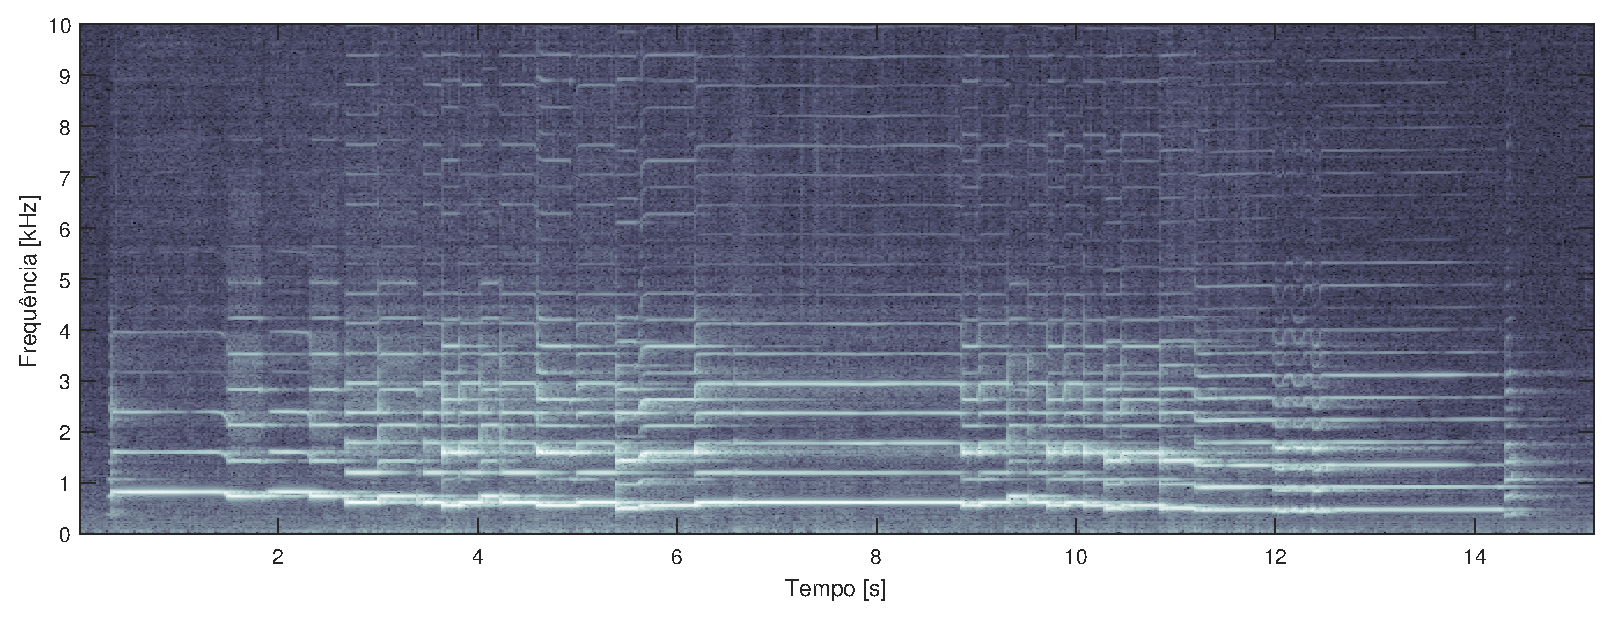
\includegraphics[width=\linewidth]{wiener/wiener-reference-signal.eps}
	\caption[Espetrograma do sinal original usado nos experimentos]{Espectrograma do sinal original utilizado nos experimentos.}
	\label{fig:wf:spectogram-reference}
\end{figure}
\begin{figure}[!ht]
	\centering
	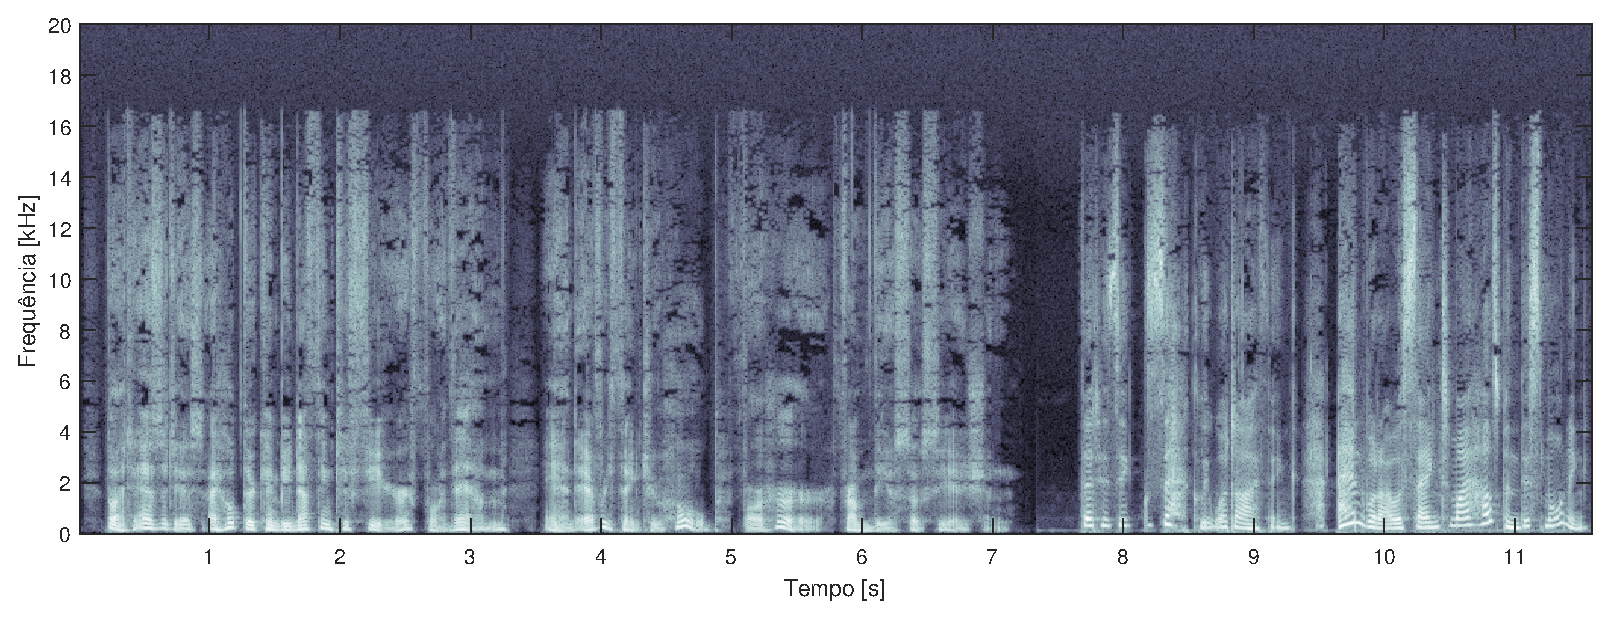
\includegraphics[width=\linewidth]{wiener/wiener-dialogue-signal.eps}
	\caption[Espetrograma do ruído usado nos experimentos]{Espectrograma da gravação de diálogo (a ser interpretada como ruído) utilizada nos experimentos.}
	\label{fig:wf:spectogram-dialogue}
\end{figure}

Em relação à janela escolhida para o método de \textit{overlap-add}, foi priorizado um
janelamento que aplicasse ganho unitário ao sinal sintetizado, para que não fosse
necessário um pós-processamento de correção de ganho. Nas devidas condições, a função
de Hann de comprimento $M$ definida como
\begin{equation}
	h^2[n] = \frac{1}{2} - \frac{1}{2}\cos\left(\frac{2\pi n}{M}\right) = \sen^2\left( \frac{\pi n}{M} \right),\ 0 \leq n \leq M-1,
\end{equation}
cumpre esse requisito: com $M$ par, uma sobreposição de $50\%$ ($H = M/2$) resulta em \textit{overlap-add} constante com ganho unitário~\cite{heinzel-2002}. Por este motivo, a janela estipulada foi escolhida com base na função de Hann. Porém, como explicitado na seção anterior, o janelamento será aplicado duas vezes ao sinal, e, portanto, precisamos de que sua versão quadrática satisfaça a condição de COLA. Assim, a janela $h[n]$ que foi usada é a raiz quadrada da descrita anteriormente:
\begin{equation}
	h[n] = \sqrt{\frac{1}{2} - \frac{1}{2}\cos\left(\frac{2\pi n}{M}\right)} = \sen\left( \frac{\pi n}{M} \right),\ 0 \leq n \leq  M-1.
\end{equation}

Todos os experimentos foram executados com filtros de tamanho $L = 34$, janelas de
comprimento $M = 2^{13} = 8192$ (aproximadamente $186$ ms), e, consequentemente, saltos
de $H = 4096$ amostras. Estes parâmetros foram definidos após múltiplos testes com
diferentes valores terem sido realizados. Tais escolhas apresentaram o melhor resultado
geral.

\subsection{\textit{Fades}}

Para o primeiro experimento, o sinal distorcido foi gerado aplicando-se um
\textit{fade-out} e um \textit{fade-in} no início e no final, respectivamente, da
gravação original. Para isso, foi utilizada a ferramenta de envoltória do Audacity, na
qual a transição entre ganhos é feita seguindo uma curva exponencial. Para o
\textit{fade-out}, os parâmetros do ganho foram $A_\mathrm{i} = 1$ e $A_\mathrm{f} =
	0.2$. Similarmente, no \textit{fade-in} estes parâmetros foram $A_\mathrm{i} = 0.2$ e
$A_\mathrm{f} = 1$. Ambos os efeitos duraram aproximadamente 1.5 segundo. O ruído não
foi adicionado à mixagem final. Assim, avaliamos a capacidade do método em estimar o
processamento de um sistema linear variante no tempo. Os resultados encontram-se na
Tabela~\ref{tab:wf:experiment-1}. {\def\arraystretch{1.25}\tabcolsep=10pt
\begin{table}[!ht]
	\centering
	\caption[Resultados do primeiro experimento: \textit{fades}]{Resultados do primeiro experimento.}
	\label{tab:wf:experiment-1}
	\begin{tabular}{cccc}
		\toprule
		               & SDR         & PAQM (MOS) & $\log_{10}(R_{\text{nonlin}})$ \\
		\midrule
		$(d, x)$       & $-11.57$ dB & $1.17$     & $-0.005$                       \\
		$(d, \hat{d})$ & $42.65$ dB  & $2.04$     & $-0.006$                       \\ \bottomrule
	\end{tabular}
\end{table}
}

Ao observarmos apenas os resultados da SDR, podemos concluir que o método estimou de
forma satisfatória a distorção que foi aplicada à gravação original. Por outro lado, se
considerarmos apenas a PAQM, a melhoria não parece ter sido tão satisfatória assim.
Porém, não podemos nos esquecer que a rigorosa compressão aplicada pela transformação
dos resultados de $\log_{10}(\mathcal{L}_n)$ em MOS pode resultar em valores baixos
mesmo em sinais muito similares. Assim, não podemos nos ater apenas ao valor absoluto
do resultado, e sim interpretá-lo no contexto geral; neste caso, a nota aproximadamente
dobrou de valor.

É interessante notar também a queda no valor de $\log_{10} (R_{\text{nonlin}})$ para $(d, \hat{d})$. Isto ocorreu pois o algoritmo empregado (com \textit{overlap-add}) não é estritamente linear; por exemplo, as últimas $L - 1$ amostras geradas na convolução de cada intervalo não são utilizadas no processo de estimação.\footnote{Se um sinal de comprimento $M$ é convoluído com um filtro de tamanho $L$, a saída resultante terá tamanho $M+L-1$. Porém, como a janela também tem tamanho $M$, foi necessário descartar as últimas $L-1$ amostras de cada iteração para realizarmos o \textit{overlap-add}.} Portanto, é possível que o método introduza não-linearidades indesejadas ao sinal de entrada. Mesmo assim, estas supostas distorções detectadas foram virtualmente inaudíveis.

\subsection{\textit{Fades} com ruído aditivo} \label{subsec:wiener:experiment-2}

No segundo experimento, foi considerada exatamente a mesma versão distorcida do teste
anterior. Porém, agora, à mixagem final foi somado o ruído; assim, o sinal distorcido
foi usado como trilha de fundo para o diálogo. Com isso, avalia-se a robustez do método
a sinais espúrios (com um caso extremo, já que o ruído está mais intenso que o sinal
desejado). A SNR da observação é $-9.17$~dB. Os resultados encontram-se na
Tabela~\ref{tab:wf:experiment-2}. {\def\arraystretch{1.25}\tabcolsep=10pt
\begin{table}[!ht]
	\centering
	\caption[Resultados do segundo experimento: \textit{fades} com ruído aditivo]{Resultados do segundo experimento.}
	\label{tab:wf:experiment-2}
	\begin{tabular}{cccc}
		\toprule
		               & SDR         & PAQM (MOS) & $\log_{10}(R_{\text{nonlin}})$ \\
		\midrule
		$(d, x)$       & $-11.57$ dB & $1.17$     & $-0.005$                       \\
		$(d, \hat{d})$ & $15.39$ dB  & $1.20$     & $-0.028$                       \\ \bottomrule
	\end{tabular}
\end{table}
}

Embora o algoritmo tenha melhorado as medidas, os valores pioraram quando comparados
aos do experimento anterior. Isto era esperado, visto que a trilha descorrelacionada
possuía maior energia na mixagem final. Deste modo, o método não conseguiu reproduzir
igualmente bem o processamento aplicado ao sinal original, resultando principalmente em
resquícios de ruído --- zumbidos ``metálicos'' --- nos instantes de maior intensidade
no diálogo.

\subsection{\textit{Soft clipping}}

No terceiro experimento, queremos avaliar a eficiência do método em replicar a
distorção não-linear de \textit{soft clipping}. No Audacity, a curva de limitação é uma
função definida por partes: linear entre $-0.5$ e $0.5$ e senoidal nas extremidades
(cada uma consiste em $1/8$ de um período de onda). A limitação é feita passando o
sinal por este mapeamento, que antes é normalizado para que seu valor máximo seja igual
ao pico de amplitude máximo especificado; no caso do experimento, este foi $-7.5$ dB. O
ruído não foi introduzido. Os resultados encontram-se na
Tabela~\ref{tab:wf:experiment-3}. {\def\arraystretch{1.25}\tabcolsep=10pt
\begin{table}[!ht]
	\centering
	\caption[Resultados do terceiro experimento: \textit{soft clipping}]{Resultados do terceiro experimento.}
	\label{tab:wf:experiment-3}
	\begin{tabular}{cccc}
		\toprule
		               & SDR        & PAQM (MOS) & $\log_{10}(R_{\text{nonlin}})$ \\
		\midrule
		$(d, x)$       & $19.56$ dB & $1.21$     & $-0.016$                       \\
		$(d, \hat{d})$ & $23.24$ dB & $1.22$     & $-0.016$                       \\ \bottomrule
	\end{tabular}
\end{table}
}

Podemos observar uma pequena melhora nos valores da SDR e da PAQM, e nenhuma alteração
no valor do $\log_{10}(R_{\text{nonlin}})$. Temos aqui o primeiro exemplo das
limitações do Filtro de Wiener, que não consegue reproduzir a distorção não-linear
aplicada ao sinal original; o incremento provavelmente se deu porque o algoritmo é
capaz de aplicar uma atenuação aos picos, mas não um ceifamento.

\subsection{\textit{Soft clipping} com ruído aditivo}

Neste experimento, somamos a trilha de diálogo ao sinal fabricado no experimento
anterior. É importante notar que não foi aplicado nenhum outro processamento ao sinal
distorcido, portanto, a SNR está maior do que a encontrada no
Experimento~\ref{subsec:wiener:experiment-2}, sendo $3.97$~dB. Os resultados
encontram-se na Tabela~\ref{tab:wf:experiment-4}.
{\def\arraystretch{1.25}\tabcolsep=10pt
\begin{table}[!ht]
	\centering
	\caption[Resultados do quarto experimento: \textit{soft clipping} com ruído aditivo]{Resultados do quarto experimento.}
	\label{tab:wf:experiment-4}
	\begin{tabular}{cccc}
		\toprule
		               & SDR        & PAQM (MOS) & $\log_{10}(R_{\text{nonlin}})$ \\
		\midrule
		$(d, x)$       & $19.56$ dB & $1.21$     & $-0.016$                       \\
		$(d, \hat{d})$ & $22.11$ dB & $1.20$     & $-0.022$                       \\ \bottomrule
	\end{tabular}
\end{table}
}

Observe que, mesmo com a melhoria no valor da SDR, houve uma piora nos valores das
outras duas medidas. Ao ouvir a estimação resultante, o porquê disso se torna evidente:
novamente temos resquícios do diálogo em alguns instantes do sinal estimado, mas, além
disso, possivelmente também artefatos do algoritmo, visto que, como demonstrado melhor
no próximo experimento, o método é capaz de introduzir ruídos no sinal distorcido.

\subsection{\textit{Fades} e codificação com perdas} \label{subsec:wiener:experiment-5}

Como o processo de codificação costuma ser executado ao fim de uma mixagem, após outras
distorções terem sido aplicadas, iremos utilizar o sinal distorcido do primeiro
experimento como entrada no algoritmo de codificação. A gravação de diálogo não foi
adicionada. Foi aplicada uma codificação MP3 com taxa de bits constante de 56 kbps
usando a biblioteca LAME\abbrev{LAME}{LAME \textit{Ain't an} MP3
	\textit{Encoder}}~\cite{lame-encoder}. Os resultados encontram-se na
Tabela~\ref{tab:wf:experiment-5}. {\def\arraystretch{1.25}\tabcolsep=10pt
\begin{table}[!ht]
	\centering
	\caption[Resultados do quinto experimento: \textit{fades} e codificação com perdas]{Resultados do quinto experimento.}
	\label{tab:wf:experiment-5}
	\begin{tabular}{cccc}
		\toprule
		               & SDR         & PAQM (MOS) & $\log_{10}(R_{\text{nonlin}})$ \\
		\midrule
		$(d, x)$       & $-14.77$ dB & $1.17$     & $-0.032$                       \\
		$(d, \hat{d})$ & $13.43$ dB  & $1.18$     & $-0.080$                       \\ \bottomrule
	\end{tabular}
\end{table}
}

É possível notar que, embora a SDR tenha ficado com um valor próximo ao do segundo experimento, a PAQM e o $\log_{10}(R_{\text{nonlin}})$ denunciam a baixa similaridade psicoacústica entre o sinal distorcido e o estimado (quando comparados aos outros resultados). Ademais, ao tentar reproduzir distorções não-lineares usando um sistema linear, o algoritmo introduziu artefatos na estimação, o que explica a queda significativa no valor de $\log_{10}(R_{\text{nonlin}})$.

\subsection{\textit{Fades} com ruído aditivo e codificação com perdas} \label{subsec:wiener:experiment-6}

Para este último teste, codificou-se o áudio gerado no segundo experimento: o sinal
$x[n]$ com \textit{fades} e diálogo somado. Os parâmetros da codificação foram os
mesmos do quinto experimento. É importante mencionar que, neste caso, não é possível
obter a versão isolada exata do sinal distorcido na observação, já que o processo de
codificação, por ser não-linear, utiliza uma combinação não-trivial entre a entrada e o
ruído. Por este motivo, como $d[n]$ usaremos o mesmo sinal distorcido gerado no
Experimento~\ref{subsec:wiener:experiment-5}, que pressupomos ser
\emph{aproximadamente} igual ao valor da versão do sinal presente em $y[n]$. Não foi
possível calcular a SNR dessa observação, mas podemos estimar seu limite superior como
sendo $-9.17$~dB. Os resultados encontram-se na Tabela~\ref{tab:wf:experiment-6}.
{\def\arraystretch{1.25}\tabcolsep=10pt
\begin{table}[!ht]
	\centering
	\caption[Resultados do sexto experimento: \textit{fades} com ruído aditivo e codificação com perdas]{Resultados do sexto experimento.}
	\label{tab:wf:experiment-6}
	\begin{tabular}{cccc}
		\toprule
		               & SDR         & PAQM (MOS) & $\log_{10}(R_{\text{nonlin}})$ \\
		\midrule
		$(d, x)$       & $-14.77$ dB & $1.17$     & $-0.032$                       \\
		$(d, \hat{d})$ & $11.47$ dB  & $1.18$     & $-0.087$                       \\ \bottomrule
	\end{tabular}
\end{table}
}

Os resultados são a culminação de tudo que vimos até agora nos experimentos. Se, por um
lado, o modelo consegue estimar a variação de amplitude, por outro, o processamento
não-linear --- junto à baixa razão sinal-ruído --- dificulta a estimação, sendo isso
refletido principalmente no quesito psicoacústico.

    \chapter{Filtro de Correntropia}
\label{chapter:correntropyfilter}

Agora que sabemos das capacidades e limitações --- dentro do contexto do projeto --- de um método de identificação linear consolidado, podemos partir para técnicas inovadoras desenvolvidas especificamente para sistemas não-lineares. A primeira a ser abordada é o Filtro de Correntropia~\cite{pokharel-2006, pokharel-2007}. Baseado em modelos que utilizam funções núcleo (\textit{kernel functions}), o filtro se propõe a atacar o \textit{trade-off} entre complexidade e robustez por meio de uma função denominada de correntropia~\cite{santamaria-2006}. O método é também chamado de Filtro de Wiener Não-linear, pois o Filtro de Wiener FIR discreto é usado em seu desenvolvimento, como será visto em breve.

Começaremos o capítulo revisando o conceito de funções núcleo, para que em seguida seja possível introduzir a função de correntropia. Então, o Filtro de Correntropia será formalmente deduzido. Além disso, será apresentada também uma forma matricial da solução, a qual foi desenvolvida durante o projeto; com ela, pôde-se implementar o algoritmo de forma vetorizada, reduzindo drasticamente seu tempo de execução. Em seguida, uma análise preliminar acerca do filtro será conduzida. Por fim, o modelo específico utilizado no trabalho será discutido, seguido pelos experimentos executados e seus respectivos resultados.

\section{Funções núcleo}

Antes de definirmos o que é a correntropia em si, devemos considerar o tópico mais amplo de funções núcleo. Popularizada por suas inúmeras aplicações na área de aprendizado de máquina, essa classe de funções envolve noções fundamentais de análise funcional e espaços de Hilbert em suas definições e propriedades. Ainda assim, é possível desenvolver uma discussão suficientemente ampla sobre o tema seguindo uma abordagem mais intuitiva e abstraindo-se dos detalhes técnicos. Este será o caminho que adotaremos pelo resto da seção, já que se aprofundar nessa teoria vai além do escopo do projeto. O leitor interessado encontra em~\cite{principe-2010} uma discussão mais completa acerca do assunto.

Essencialmente, uma função núcleo computa a \emph{similaridade} entre dois vetores $\mathbf{x}_1$ e $\mathbf{x}_2$ presentes no mesmo espaço vetorial $X$. Porém, ao contrário de outros operadores que visam ao mesmo objetivo --- como a norma euclidiana da diferença ou a similaridade por cosseno ---, a função implicitamente mapeia os pontos para um espaço vetorial de maior dimensão $F$, e então calcula o produto interno dos vetores transformados. A ideia por trás desse mapeamento é gerar dimensões que reflitam outros aspectos sobre os dados, e, assim, fazer com que o produto interno entre os pontos mapeados seja mais elucidativo em relação à similaridade entre $\mathbf{x}_1$ e $\mathbf{x}_2$.

Desse modo, uma \emph{função núcleo} $\kappa$ é definida~\cite{shawetaylor-2004} como sendo uma função que, para todos $\mathbf{x}_1, \mathbf{x}_2 \in X$, satisfaz
\begin{equation}
    \kappa(\mathbf{x}_1, \mathbf{x}_2) = \bm{\phi}(\mathbf{x}_1)^T \bm{\phi}(\mathbf{x}_2),
    \symbl{$\kappa$}{Função núcleo}
    \symbl{$\bm{\phi}$}{Transformação vetorial associada à função núcleo}
\end{equation}
onde $\bm{\phi}$ é uma função vetorial definida por
\begin{equation}
    \bm{\phi} : \mathbf{x} \in X \subseteq \mathbb{R}^p \longmapsto \bm{\phi}(\mathbf{x}) \in F \subseteq \mathbb{R}^P.
\end{equation}
Para que a estratégia faça sentido, $P \geq p$. É importante notar que \emph{não é preciso conhecer o mapeamento $\bm{\phi}$ associado à função núcleo.} Na verdade, a força do método é justamente essa: usando um núcleo válido\footnote{Um ``núcleo válido'', ou núcleo de Mercer~\cite{principe-2010}, é contínuo, simétrico e positivo definido. Note que, por causa da simetria, podemos afirmar que $\kappa(\mathbf{x}_1, \mathbf{x}_2) = \kappa(\mathbf{x}_2, \mathbf{x}_1)$.}, calcula-se diretamente o produto interno entre dois vetores em $F$, sem aplicar a função $\bm{\phi}$.

Vamos ilustrar a capacidade das funções núcleo por meio de um exemplo. Considere os vetores $\mathbf{x}_1, \mathbf{x}_2 \in \mathbb{R}^2$ descritos por
\begin{equation}
    \mathbf{x}_1 = \begin{bmatrix} \alpha_1\\\beta_1 \end{bmatrix},\ \mathbf{x}_2 = \begin{bmatrix} \alpha_2\\\beta_2 \end{bmatrix}.
\end{equation}

Para calcularmos a semelhança entre os vetores, em vez de usarmos o produto interno convencional, usaremos o núcleo polinomial~\cite{principe-2010} de segunda ordem $\kappa(\mathbf{x}_1, \mathbf{x}_2) = ( \mathbf{x}_1^T \mathbf{x}_2 + 1)^2$. Assim,
\begin{align}
    \kappa(\mathbf{x}_1, \mathbf{x}_2) &= (\alpha_1 \alpha_2 + \beta_1 \beta_2 + 1)^2\\
                                       &= \alpha_1^2 \alpha_2^2 + 2 \alpha_1 \alpha_2 + 2 \alpha_1 \alpha_2 \beta_1 \beta_2 + 2 \beta_1 \beta_2 + \beta_1^2 \beta_2^2 + 1\\
                                       &= \bm{\phi}(\mathbf{x}_1)^T \bm{\phi}(\mathbf{x}_2);
\end{align}
nesse caso, a função $\bm{\phi}$ implicitamente aplicada pelo núcleo foi
\begin{equation}
    \bm{\phi}(\mathbf{x}_i) = \begin{bmatrix}
        \alpha_i^2 &
        \sqrt{2}\alpha_i &
        \sqrt{2}\alpha_i\beta_i &
        \sqrt{2}\beta_i &
        \beta_i^2 &
        1
    \end{bmatrix}^T.
\end{equation}

Note que $\bm{\phi}(\mathbf{x}_i)$ contém mais informações do que $\mathbf{x}_i$, embora os dados de origem sejam os mesmos. Com $\bm{\phi}(\mathbf{x}_i)$, poderíamos, por exemplo, modelar um sistema quadrático com um algoritmo linear, visto que os termos quadráticos já estão presentes no vetor de entrada. Em outras palavras, \emph{certas relações não-lineares em $X$ se tornam lineares em $F$}. Podemos generalizar essa estratégia para qualquer tipo de núcleo, com a restrição de que normalmente teremos apenas $\kappa$, exigindo então que o algoritmo trabalhe não com vetores individuais, mas com seus produtos internos.

Uma das funções núcleo mais importantes --- quiçá a mais importante --- é a gaussiana invariante à translação~\cite{santamaria-2006}, definida como sendo\footnote{A função é normalmente definida sem o fator multiplicativo $1/\sqrt{2\pi}\sigma$, mas como em~\cite{santamaria-2006} o termo está presente, ele também se encontra na nossa definição.}
\begin{equation}
    \kappa(\mathbf{x}_1, \mathbf{x}_2) = \frac{1}{\sqrt{2\pi} \sigma} \exp\left( - \frac{\lVert \mathbf{x}_1 - \mathbf{x}_2 \rVert^2}{2\sigma^2} \right),\symbl{$\sigma$}{Parâmetro do núcleo gaussiano}
\end{equation}
onde $\sigma$ é um parâmetro ajustável. A principal característica deste núcleo é que seu mapeamento $\bm{\phi}$ associado gera um espaço $F$ de dimensão infinita, o que torna computacionalmente impossível calcular $\bm{\phi}(\mathbf{x})$ explicitamente. Além disso, algumas outras particularidades desse núcleo o fazem ser usado na função de correntropia, como veremos a seguir.

Em suma, núcleos são usados para calcular a semelhança entre dois vetores considerando transformações não-lineares aplicadas sobre seus elementos. Com eles, podemos tentar fazer com que relações não-lineares em um espaço vetorial se tornem lineares em outro, o que possibilita a aplicação de métodos mais simples na solução de problemas. Embora poderosas, essas funções não podem ser usadas em qualquer algoritmo linear; é preciso que este trabalhe com produtos internos para que, assim, as ocorrências de $\mathbf{x}_1^T\mathbf{x}_2$ sejam substituídas por um núcleo $\kappa(\mathbf{x}_1, \mathbf{x}_2)$ apropriado.

\section{Função de correntropia}

Agora que possuímos um melhor entendimento sobre funções núcleo, a função de correntropia pode ser formalmente apresentada.

Seja $\{\mathbf{x}[n]\}$ uma sequência estocástica, com $n$ sendo o índice associado ao elemento do conjunto, e $\mathbf{x}[n] \in \mathbb{R}^p$, $p \in \mathbb{N}^*$. A função de correlação generalizada, ou simplesmente \emph{correntropia}, é uma função $V : \mathbb{R}^p \times \mathbb{R}^p \mapsto \mathbb{R}$ definida~\cite{santamaria-2006} por
\begin{equation}
    V_{\textbf{x}\textbf{x}}[n_1, n_2] = E\{ \kappa(\mathbf{x}[n_1], \mathbf{x}[n_2]) \},
    \symbl{$V_{\cdot\cdot}{[k]}$}{Função de correntropia}
\end{equation}
onde $\kappa$ é um núcleo válido e $E\{\cdot\}$ é o operador de valor esperado estatístico. Como tanto em~\cite{santamaria-2006} quanto em~\cite{pokharel-2006} o núcleo utilizado é o gaussiano, este também será o qual usaremos pelo restante do capítulo. É importante mencionar que, assim como a função núcleo utilizada para sua concepção --- independente de qual seja, contanto que seja válida ---, a correntropia é uma função simétrica positiva definida.

O que faz a função de correntropia ser tão interessante? Em primeiro lugar, a partir da discussão sobre núcleos da seção anterior, podemos afirmar que a correntropia calcula a similaridade média entre dois instantes de uma sequência considerando complexas características não-lineares. Além disso, se expandirmos o núcleo gaussiano em uma série de potências, encontramos
\begin{equation}
    V_{\textbf{x}\textbf{x}}[n_1, n_2] = \frac{1}{\sqrt{2\pi}\sigma} \sum_{i=0}^\infty \frac{(-1)^i}{2^i \sigma^{2i} i!} E\{ \lVert \mathbf{x}[n_1] - \mathbf{x}[n_2] \rVert^{2i} \}.
    \label{eq:correntropy:series-expansion}
\end{equation}
Note que todos os momentos pares da variável aleatória $\lVert\mathbf{x}[n_1] - \mathbf{x}[n_2]\rVert$ estão presentes na série. Mais especificamente, o termo em $i=1$ é proporcional a
\begin{equation}
    E\{ \lVert \mathbf{x}[n_1] - \mathbf{x}[n_2] \rVert^2 \} = E\{ \lVert \mathbf{x}[n_1] \rVert^2 \} + E\{ \lVert \mathbf{x}[n_2] \rVert ^2 \} - 2 E\{ \mathbf{x}[n_1]^T \mathbf{x}[n_2]\},
    \label{eq:correntropy:expansion-1st-term}
\end{equation}
e, como $E\{ \mathbf{x}[n_1]^T \mathbf{x}[n_2] \} = R_{\mathbf{x}\mathbf{x}}[n_1, n_2]$, podemos concluir que as informações associadas à autocorrelação (ou correlação cruzada) estão presentes na função. Ademais, se a sequência tiver média zero, a Equação~\eqref{eq:correntropy:expansion-1st-term} demonstra que a função também incluirá informações acerca das variâncias nos instantes considerados (e a autocorrelação se tornará a covariância).

Ainda analisando a Equação~\eqref{eq:correntropy:series-expansion}, é possível concluir que, para que a correntropia dependa apenas do intervalo entre $n_1$ e $n_2$, é preciso que todos os momentos pares de $\lVert\mathbf{x}[n_1] - \mathbf{x}[n_2]\rVert$ sejam constantes. Uma condição suficiente para isso é que a sequência aleatória $\{\mathbf{x}[n]\}$ seja estacionária no sentido estrito (SSS, de \textit{Strict-Sense Stationary}\abbrev{SSS}{\textit{Strict-Sense Stationary}})~\cite{peebles-1987}. Deste modo, $V_{\textbf{x}\textbf{x}}$ dependerá apenas do intervalo $k = n_2 - n_1$. A função $V_{\textbf{x}\textbf{x}}[k]$ é positiva, simétrica, e com valor máximo na origem.

Supondo a condição de estacionariedade estrita, a correntropia de uma sequência finita de $N$ amostras pode ser estimada por meio da média amostral:
\begin{equation}
    \hat{V}_{\textbf{x}\textbf{x}}[k] = \frac{1}{N - k + 1} \sum_{n=k}^{N-1} \kappa(\textbf{x}[n], \textbf{x}[n-k]).
\end{equation}
Este estimador é não-enviesado e assintoticamente consistente~\cite{santamaria-2006}, e foi o utilizado para o cálculo da correntropia nos experimentos deste capítulo.

E por que o nome de correntropia? Uma outra importante característica da função, omitida neste texto por não ter relevância para o projeto, envolve uma aplicação no contexto de teoria da informação. Assim, o nome \emph{correntropia} é uma aglutinação de \emph{correlação} com \emph{entropia}, duas informações que a estatística contém.

\section{Filtro de Correntropia}
\label{section:correntropy:filter}

Estamos finalmente munidos de todas as ferramentas necessárias para deduzirmos o Filtro de Correntropia. É importante frisar que o Filtro de Wiener FIR causal é empregado em sua modelagem, e como esse sistema já foi apresentado no Capítulo~\ref{chapter:wiener}, a discussão não será secundada aqui.

Nosso ponto de partida para a dedução do modelo será um teorema envolvendo a função de correntropia. Dada uma sequência estocástica estacionária $x[n]$ --- por exemplo, o sinal observado no Filtro de Wiener --- e sua correntropia $V_{xx}[n_1, n_2]$, o teorema~\cite{pokharel-2006} afirma que existe um mapeamento $z : \mathbb{R} \mapsto \mathbb{R}$ tal que
\begin{equation}
    V_{xx}[n_1, n_2] = E \{ z(x[n_1]) z(x[n_2]) \}.
    \label{eq:correntropy:theorem}
\end{equation}
Em outras palavras, a correntropia de $x[n]$ é a autocorrelação da sequência aleatória $z(x[n])$. A prova dessa afirmação, que envolve expandir as funções em autofunções e autovalores, pode ser encontrada em~\cite{pokharel-2006}.

Como vimos na Seção~\ref{section:wiener:fir-filter}, os coeficientes do Filtro de Wiener são computados por meio da matriz de correlação do sinal de entrada. Então, se modelarmos o filtro utilizando a sequência $z(x[n])$ como entrada, será possível usar a correntropia do sinal observado. Desse modo, sejam $x[n]$ o sinal observado e $d[n]$ o sinal desejado, assim como definido no Capítulo~\ref{chapter:wiener}. Além disso, seja $L$ o tamanho do filtro. O vetor de entrada $\mathbf{z}[n]$, definido como sendo
\begin{equation}
    \mathbf{z}[n] = \begin{bmatrix}
       z(x[n]) & z(x[n - 1]) & \cdots & z(x[n - L + 1])
    \end{bmatrix}^T,
    \symbl{$\mathbf{z}{[n]}$}{Vetor de entrada do Filtro de Correntropia}
\end{equation}
resulta nos seguintes coeficientes ótimos para o Filtro de Wiener FIR causal:
\begin{equation}
    \mathbf{w}^* = \mathbf{R}_{zz}^{-1} \mathbf{r}_{zd}.
\end{equation}

Com base no teorema apresentado, podemos substituir a matriz $\mathbf{R}_{zz}$ pela \emph{matriz de correntropia} de $x[n]$. Supondo que o sinal é estacionário no sentido estrito, a matriz é definida como sendo
\begin{equation}
    \mathbf{V}_{xx} = \begin{bmatrix}
        V_{xx}[0] & V_{xx}[1] & \cdots & V_{xx}[L - 1]\\
        V_{xx}[1] & V_{xx}[0] & \cdots & V_{xx}[L - 2]\\
        \vdots & \vdots & \ddots & \vdots\\
        V_{xx}[L-1] & V_{xx}[L-2] & \cdots & V_{xx}[0]
    \end{bmatrix}.
    \symbl{$\mathbf{V}_{\cdot\cdot}$}{Matriz de correntropia}
\end{equation}

Assim, a saída do filtro será
\begin{equation}
    \hat{d}[n] = \mathbf{z}[n]^T \mathbf{V}_{xx}^{-1} \mathbf{r}_{zd}.
    \label{eq:correntropy:yn-with-z}
\end{equation}

A Equação~\eqref{eq:correntropy:yn-with-z} apresenta o resultado do filtro em função da sequência $z(x[n])$, a qual não conhecemos. Para descrevermos a equação puramente em função de $x[n]$, devemos primeiramente substituir $\mathbf{r}_{zd}$ por um estimador. Supondo ergodicidade, o vetor pode ser aproximado por sua média temporal,
\begin{equation}
    \hat{\mathbf{r}}_{zd} = \frac{1}{N} \sum_{k=0}^{N-1} d[k] \mathbf{z}[k].
\end{equation}
Então, fazendo a substituição e depois expandindo os produtos vetoriais em~\eqref{eq:correntropy:yn-with-z}, encontramos que
\begin{align}
    \hat{d}[n] &= \mathbf{z}[n]^T \mathbf{V}_{xx}^{-1} \mathbf{r}_{zd}\\
         &\simeq \mathbf{z}[n]^T \mathbf{V}_{xx}^{-1} \frac{1}{N} \sum_{k=0}^{N-1} d[k] \mathbf{z}[k]\\
         &= \frac{1}{N} \sum_{k=0}^{N-1} \sum_{i=0}^{L-1} \sum_{j=0}^{L-1} z(x[n-i]) \Tilde{v}_{ij} d[k] z(x[k-j])\\
         &= \frac{1}{N} \sum_{k=0}^{N-1} d[k] \sum_{i=0}^{L-1} \sum_{j=0}^{L-1} \Tilde{v}_{ij} z(x[n-i]) z(x[k-j])\\
         &\simeq \frac{1}{N} \sum_{k=0}^{N-1} d[k] \sum_{i=0}^{L-1} \sum_{j=0}^{L-1} \Tilde{v}_{ij} \kappa(x[n-i], x[k-j]),
         \label{eq:correntropy:filter}
\end{align}
onde $\Tilde{v}_{ij}$\symbl{$\Tilde{v}_{ij}$}{Elemento na $i$-ésima linha e $j$-ésima coluna do inverso da matriz de correntropia} é o elemento da $i$-ésima linha e $j$-ésima coluna de $\mathbf{V}_{xx}^{-1}$. A expressão final é encontrada aproximando-se $z(x[n-i]) z(x[k-j])$ por $\kappa(x[n-i], x[k-j])$, que é uma aproximação válida na média de acordo com a Equação~\eqref{eq:correntropy:theorem}.

O Filtro de Correntropia é totalmente caracterizado pela Equação~\eqref{eq:correntropy:filter}; com ela, calcula-se a $n$-ésima amostra da estimação. A Figura~\ref{fig:correntropy:filter} ilustra este processo, considerando que o inverso da matriz de correntropia já foi computado, e usando versões vetoriais de $x[n]$, como definido na Equação~\eqref{eq:wf:xn-vector}. Em~\cite{pokharel-2006, pokharel-2007}, menciona-se uma etapa adicional em que se iguala a variância de $\hat{d}[n]$ com a de $d[n]$ por meio de uma correção de ganho, e que essa disparidade é muito provavelmente resultado da aproximação feita no último passo da modelagem do filtro. Nos testes do projeto, foi observado que essa correção é \emph{essencial} para a obtenção de resultados satisfatórios.
\begin{figure}[!ht]
    \centering
     \begin{subfigure}[t]{\textwidth}
        \centering
        \begin{tikzpicture}[node distance=0.75cm and 2cm]
    % x[0] row
    \node[dspnodeopen, dsp/label=above] (x-0) {$\textbf{x}[0]$};
    \node[dspfilter, below=of x-0, yshift=0.25cm] (block-0) {$S$};
    \draw[dspconn] (x-0) -- (block-0);
    
    \node[dspmixer, right=of block-0] (prod-0) {};
    \node[dspnodeopen, dsp/label=above, above=of prod-0] (d-0) {$d[0]$};
    \draw[dspconn] (d-0) -- (prod-0);
    \draw[dspconn] (block-0) -- (prod-0);

    % x[1] row
    \node[dspnodeopen, dsp/label=above, below=of block-0, yshift=-0.25cm] (x-1) {$\textbf{x}[1]$};
    \node[dspfilter, below=of x-1, yshift=0.25cm] (block-1) {$S$};
    \draw[dspconn] (x-1) -- (block-1);
    
    \node[dspmixer, right=of block-1] (prod-1) {};
    \node[dspnodeopen, dsp/label=above, above=of prod-1] (d-1) {$d[1]$};
    \draw[dspconn] (d-1) -- (prod-1);
    \draw[dspconn] (block-1) -- (prod-1);
    
    \node[below=of block-1, yshift=0.75cm] (vdots-blocks) {$\vdots$};
    \node[below=of prod-1, yshift=0.47cm] (vdots-prods) {$\vdots$};
    
    % x[N-1] row
    \node[dspnodeopen, dsp/label=above, below=of vdots-blocks, yshift=0cm] (x-N) {$\textbf{x}[N-1]$};
    \node[dspfilter, below=of x-N, yshift=0.25cm] (block-N) {$S$};
    \draw[dspconn] (x-N) -- (block-N);

    \node[dspmixer, right=of block-N] (prod-N) {};
    \node[dspnodeopen, dsp/label=above, above=of prod-N] (d-N) {$d[N-1]$};
    \draw[dspconn] (d-N) -- (prod-N);
    \draw[dspconn] (block-N) -- (prod-N);

    % Connections and other stuff
    \node[dspadder, right=of prod-1] (adder) {};
    \node[dspmixer, right=of adder, xshift=-1cm] (div) {};
    
    \node[dspnodeopen, dsp/label=left, left=of block-1] (x-n) {$\textbf{x}[n]$};
    \node[coordinate, left=of block-0, xshift=2cm] (xcord-0) {};
    \node[coordinate, left=of block-N, xshift=2cm] (xcord-N) {};
    \draw[dspconn] (x-n) -- (xcord-0);
    \draw[dspconn] (x-n) -- (block-1);
    \draw[dspconn] (x-n) -- (xcord-N);

    \draw[dspconn] (prod-0) -- (adder);
    \draw[dspconn] (prod-1) -- (adder);
    \draw[dspconn] (prod-N) -- (adder);
    
    \draw[dspconn] (adder) -- (div);
    \node[dspnodeopen, dsp/label=left, above=of div, yshift=-0.25cm] (div-N) {};
    \node[yshift=-0.75cm, above=of div-N] (div-N-label) {$\displaystyle\frac{1}{N}$};
    \node[dspnodeopen, dsp/label=above, right=of div, xshift=-1cm] (y-n) {$\hat{d}[n]$};
    \draw[dspconn] (div) -- (y-n);
    \draw[dspconn] (div-N) -- (div);
\end{tikzpicture}
        \caption{Diagrama de blocos para o cálculo da $n$-ésima amostra.}
        \label{fig:correntropy:block-diagram}
    \end{subfigure}

    \bigskip\medskip

    \begin{subfigure}[t]{\textwidth}
        \centering
        \begin{tikzpicture}[node distance=0.75cm and 1cm]
    \node[dspfilter, minimum height=2cm, minimum width=9cm, text height=0.3cm] (sigma) {
        \footnotesize
        \begingroup
        \setlength\arraycolsep{5pt}
        $\begin{matrix}
        \Tilde{v}_{00} \kappa(x[n], x[k]) & \cdots & \Tilde{v}_{0L-1} \kappa(x[n], x[k-L+1])\\
        \vdots & \ddots & \vdots\\
        \Tilde{v}_{L-10} \kappa(x[n-L+1], x[k]) & \cdots & \Tilde{v}_{L-1L-1} \kappa(x[n-L+1], x[k-L+1])
        \end{matrix}$
        \endgroup
    };

    \node[dspnodeopen, dsp/label=above, left=of sigma] (x-n) {$\textbf{x}[n]$};
    \node[dspnodeopen, dsp/label=left, above=of sigma] (x-i) {$\textbf{x}[k]$};

    \draw[dspconn] (x-n) -- (sigma);
    \draw[dspconn] (x-i) -- (sigma);
    \node[coordinate, right=of sigma, xshift=1cm, inner sep=0pt] (sum-cord) {};
    \draw[dspconn] (sigma) -- node[midway,above] {$\sum_i \sum_j s_{ij}$} (sum-cord);
\end{tikzpicture}

        \caption{Detalhamento do bloco $S$ do diagrama.}
        \label{fig:correntropy:sigma-specification}
    \end{subfigure}

    \caption[Diagrama de blocos do Filtro de Correntropia]{Diagrama de blocos que ilustra o algoritmo do Filtro de Correntropia, e detalhe do bloco $S$; $\mathbf{x}[k]$ é um vetor como definido em~\eqref{eq:wf:xn-vector}. Ilustrações baseadas em desenhos similares presentes em~\cite{pokharel-2007}.}
    \label{fig:correntropy:filter}
\end{figure}

\subsection{Solução matricial}

A Equação~\eqref{eq:correntropy:filter} apresenta um problema operacional grave: a complexidade para se calcular uma amostra da saída, mesmo com o inverso da matriz de correntropia já computado, é $O(N L^2)$; consequentemente, a complexidade para gerarmos a estimação em sua totalidade é $O(N^2 L^2)$. Isso ocorre porque não temos coeficientes explícitos associados ao filtro, diferentemente do Filtro de Wiener. Para uma gravação de áudio de alta qualidade, que normalmente contém mais de 40 mil amostras por segundo, uma complexidade tão alta se torna um obstáculo para o desenvolvimento do projeto.

Para mitigar esse problema, podemos tentar reescrever a Equação~\eqref{eq:correntropy:filter} como uma expressão matricial. Assim, embora o algoritmo continue sendo de alta complexidade, ele poderá ser vetorizado, resultando num ganho computacional considerável em máquinas que suportem esse tipo de operação.

Começaremos definindo a \emph{matriz núcleo} de $x[n]$, a qual será representada por $\mathbf{K}_{xx}$. Esta matriz é quadrada, simétrica, com dimensões $N \times N$ (ou seja, sem as condições iniciais nulas de $x[n]$), e seus elementos são definidos por
\begin{equation}
     (\mathbf{K}_{xx})_{ij} = \kappa(x[N - 1 - i], x[N - 1 - j]).
     \symbl{$\mathbf{K}_{\cdot\cdot}$}{Matriz núcleo}
\end{equation}

Com a matriz núcleo, é possível computar todos os somatórios associados aos índices $i$ e $j$ na Equação~\eqref{eq:correntropy:filter} em ``uma operação só'', realizando uma convolução matricial\footnote{Normalmente, em uma convolução matricial, uma das matrizes tem suas linhas e colunas invertidas antes do processo, de modo similar ao que acontece no caso funcional. Na nossa aplicação, porém, essa inversão não é aplicada.} entre $\textbf{V}_{xx}^{-1}$ e $\mathbf{K}_{xx}$. Em outras palavras,
\begin{equation}
    (\textbf{V}_{xx}^{-1} * \mathbf{K}_{xx})_{ij} = \sum_{p=i}^{i+L-1} \sum_{q=j}^{j+L-1} \Tilde{v}_{(p-i)(q-j)} \kappa(x[N - 1 - p], x[N - 1 - q]).
\end{equation}
Antes da convolução, é feito um \textit{zero padding} assimétrico em $\mathbf{K}_{xx}$, adicionando $L-1$ linhas nulas abaixo e $L-1$ colunas nulas à direita da matriz. Assim, o resultado da convolução é uma matriz de dimensões $N \times N$.

Finalmente, definindo $\mathbf{d} \in \mathbb{R}^N$ como sendo o vetor com todas as amostras do sinal desejado, ou seja,
\begin{equation}
    \mathbf{d} = \begin{bmatrix}
        d[N-1] & d[N-2] & \cdots & d[1] & d[0]
    \end{bmatrix}^T,
    \symbl{$\mathbf{d}$}{Vetor com todas as amostras do sinal desejado}
\end{equation}
o Filtro de Correntropia pode então ser representado da seguinte forma:
\begin{equation}
    \hat{\mathbf{d}} = \frac{1}{N} (\textbf{V}_{xx}^{-1} * \mathbf{K}_{xx}) \mathbf{d}.
\end{equation}

\section{Testes preliminares}

Se comparado a outros métodos mais consolidados --- como o próprio Filtro de Wiener, por exemplo ---, o Filtro de Correntropia é um modelo ainda pouco explorado. Isto é corroborado pela literatura consultada para o projeto, na qual não há uma discussão suficientemente satisfatória acerca das capacidades e limitações do algoritmo. Por esse motivo, é interessante que façamos uma análise preliminar do filtro; assim, conseguiremos identificar suas particularidades, o que idealmente facilitará não somente a modelagem do sistema de estimação, como também a interpretação dos resultados dos experimentos.

Em nossos testes, usaremos dois sinais principais; ambos mais simples do que as gravações sonoras utilizadas nos experimentos finais, mas não menos significativos. O primeiro é composto pelo somatório de cinco senoides, uma delas assumindo a frequência fundamental de 3~Hz, e as restantes representando os quatro harmônicos subsequentes. A forma de onda resultante, a qual foi amostrada a uma frequência de $f_s =$ 2~kHz durante 1~s, se encontra na Figura~\ref{fig:correntropy:sinewave}. Por se tratar de um sinal suave, será possível avaliar graficamente a eficiência do método, sem precisarmos nos basear apenas em medidas numéricas.

\begin{figure}[!ht]
    \centering
    \begin{tikzpicture}
    \begin{axis}[
        xmin=0, xmax=1,
        ymin=-1, ymax=1,
        xtick={0,0.25,0.5,0.75,1},
        ytick={-1,-0.5,0,0.5,1},
        grid=major,
        width=\linewidth,
        height=7cm
    ]

        \addplot[
            color=black,
            very thick
        ] plot table {data/correntropy-sinewave.dat};

    \end{axis}
\end{tikzpicture}

    \caption[Forma de onda gerada a partir de senoides utilizada nos experimentos preliminares do Filtro de Correntropia]{Forma de onda utilizada nos experimentos preliminares do Filtro de Correntropia, gerada a partir de senoides. Uma dessas senoides está na frequência fundamental de 3~Hz, e as outras assumem os quatro harmônicos consecutivos: 6~Hz, 9~Hz, 12~Hz e 15~Hz. As amplitudes dos componentes foram omitidas aqui por falta de relevância, mas podem ser encontradas no código do projeto~\cite{nonlinear-filters-repo}.}
    \label{fig:correntropy:sinewave}
\end{figure}

O segundo sinal a ser utilizado é um modelo autorregressivo (AR\abbrev{AR}{Autorregressivo}). Uma forma comum de se modelar sinais é por meio de um sistema fonte-filtro, em que a entrada é um ruído branco e a resposta em frequência do filtro representa o espectro do sinal desejado. O modelo AR é baseado em um filtro do tipo só-polos, no qual as raízes do denominador definem o espectro. Este sistema é muito usado em processamento de áudio porque a maioria das emissões sonoras envolve ressonâncias --- ou seja, polos~\cite{godsill-2002}. Deste modo, ao usarmos este modelo nos testes, poderemos ter uma primeira impressão de como o algoritmo se comporta com gravações sonoras. O sinal foi gerado com um filtro de ordem 80 (40 pares de polos), a uma taxa de amostragem de $f_s = 44.1$~kHz durante 200~ms, e sua faixa de valores foi limitada em $[-1, 1]$, assim como em sinais de áudio digitais.

Como o modelo autorregressivo resulta em uma forma de onda de aparência ruidosa, não será possível avaliar a eficácia do filtro graficamente como faremos com a entrada senoidal. Por isso, metrificaremos numericamente a qualidade da estimação com a SDR, que pode ser prontamente generalizada para quaisquer dois sinais unidimensionais. Além disso, também tentaremos estimar os sinais com o Filtro de Wiener, para que possamos observar se o Filtro de Correntropia é melhor, pior, ou tão bom quanto um filtro linear ótimo (para as condições propostas).

\subsection{Experimento: estimação linear}

O primeiro experimento visou a avaliar a capacidade do filtro de reproduzir distorções lineares. Para isso, os sinais de teste foram ambos filtrados pelo mesmo passa-baixas: uma média móvel de ordem 150. Porém, para tornar o experimento mais interessante, foi estipulado que ambos os filtros testados tivessem ordem $L = 10$, um valor substancialmente menor do que a ordem do sistema a ser reproduzido. O valor considerado ótimo para o parâmetro do núcleo gaussiano foi $\sigma = 1 \times 10^{-10}$. Os resultados do experimento se encontram na Tabela~\ref{tab:correntropy:poc-experiment-1}; na Figura~\ref{fig:correntropy:poc-experiment-1}, encontram-se as formas de onda estimadas pelos filtros para o sinal senoidal.
{\def\arraystretch{1.25}\tabcolsep=10pt
\begin{table}[!ht]
    \centering
    \caption[Resultados do primeiro experimento preliminar: estimação linear]{Resultados, em SDR, do primeiro experimento preliminar.}
    \label{tab:correntropy:poc-experiment-1}
    \begin{tabular}{cccc}
        \toprule
                    & Original & Wiener       & Correntropia  \\ \midrule
        Senoides    & $-2.99$ dB & $3.10$ dB    & $41.06$ dB    \\
        Modelo AR   & $-46.30$ dB & $3.24$ dB    & $75.54$ dB    \\ \bottomrule
    \end{tabular}
\end{table}
}
\begin{figure}[!ht]
    \centering
    \begin{tikzpicture}
    \begin{axis}[
        xmin=0, xmax=1,
        ymin=-1, ymax=1,
        xtick={0,0.25,0.5,0.75,1},
        ytick={-1,-0.5,0,0.5,1},
        grid=major,
        width=\linewidth,
        height=7cm,
        legend style={font=\footnotesize, at={(0.98,0.95)}, anchor=north east}
    ]

        \addplot[
            color=lightgray,
            very thick,
            densely dotted
        ] plot table {data/correntropy-sinewave.dat};
        \addlegendentry{Original}

        \addplot[
            color=black,
            very thick
        ] plot table[x index=0, y index=1] {data/correntropy-poc-experiment-1.dat};
        \addlegendentry{Desejado}

        \addplot[
            color=gray,
            very thick
        ] plot table[x index=0, y index=2] {data/correntropy-poc-experiment-1.dat};
        \addlegendentry{Wiener}

        \addplot[
            color=lightgray,
            very thick,
            densely dashed
        ] plot table[x index=0, y index=3] {data/correntropy-poc-experiment-1.dat};
        \addlegendentry{Correntropia}
    \end{axis}
\end{tikzpicture}

    \caption[Saída desejada e estimações do primeiro experimento preliminar]{Gráfico com a saída desejada (quando a entrada é o somatório de senoides) e as estimações computadas pelos filtros para o primeiro experimento preliminar com o Filtro de Correntropia.}
    \label{fig:correntropy:poc-experiment-1}
\end{figure}

Como podemos observar, o Filtro de Correntropia conseguiu estimar melhor as saídas desejadas, mesmo com ordem reduzida. Dois fatores possivelmente explicam esse fenômeno: em primeiro lugar, tem-se o mapeamento infinito realizado pelo núcleo gaussiano, o que pode ter compensado a menor ordem; além disso, o filtro pode ter feito melhor proveito das amostras do sinal desejado, já que estas são usadas diretamente na geração das amostras da estimação (ao contrário do Filtro de Wiener, que as usa somente no cálculo do vetor de correlação cruzada).

\subsection{Experimento: estimação não-linear}

Neste experimento, queremos observar a capacidade de estimação de distorções não-lineares do filtro, o principal motivador deste capítulo. Para isso, os sinais de teste foram processados por uma função de \textit{soft clipping} definida por
\begin{equation}
    f(x) = \frac{2}{\pi} \arctan(1.5 x),
\end{equation}
a qual apresenta comportamento aproximadamente linear em torno da origem, e comprime sinais na faixa de $[-1, 1]$ para a faixa de $[-0.63, 0.63]$. A ordem definida para o Filtro de Wiener foi de $L = 34$, ao passo que para o Filtro de Correntropia a ordem com os melhores resultados foi de $L = 1$, em conjunto com um desvio de $\sigma = 0.9$. As notas se encontram na Tabela~\ref{tab:correntropy:poc-experiment-2}; na Figura~\ref{fig:correntropy:poc-experiment-2}, as formas de onda estimadas para o sinal senoidal são apresentadas.
{\def\arraystretch{1.25}\tabcolsep=10pt
\begin{table}[!ht]
    \centering
    \caption[Resultados do segundo experimento preliminar: estimação não-linear]{Resultados, em SDR, do segundo experimento preliminar.}
    \label{tab:correntropy:poc-experiment-2}
    \begin{tabular}{cccc}
        \toprule
                    & Original & Wiener        & Correntropia      \\ \midrule
        Senoides    & $8.72$ dB & $20.05$ dB    & $33.59$ dB        \\
        Modelo AR   & $11.96$ dB & $20.14$ dB    & $31.59$ dB        \\ \bottomrule
    \end{tabular}
\end{table}
}
\begin{figure}[!ht]
    \centering
    \begin{tikzpicture}
    \begin{axis}[
        xmin=0, xmax=1,
        ymin=-1, ymax=1,
        xtick={0,0.25,0.5,0.75,1},
        ytick={-1,-0.5,0,0.5,1},
        grid=major,
        width=\linewidth,
        height=7cm,
        legend style={font=\footnotesize, at={(0.98,0.95)}, anchor=north east}
    ]

        \addplot[
            color=lightgray,
            very thick,
            densely dotted
        ] plot table {data/correntropy-sinewave.dat};
        \addlegendentry{Original}

        \addplot[
            color=black,
            very thick
        ] plot table[x index=0, y index=1] {data/correntropy-poc-experiment-2.dat};
        \addlegendentry{Desejado}

        \addplot[
            color=gray,
            very thick
        ] plot table[x index=0, y index=2] {data/correntropy-poc-experiment-2.dat};
        \addlegendentry{Wiener}

        \addplot[
            color=lightgray,
            very thick,
            densely dashed
        ] plot table[x index=0, y index=3] {data/correntropy-poc-experiment-2.dat};
        \addlegendentry{Correntropia}
    \end{axis}
\end{tikzpicture}

    \caption[Saída desejada e estimações do segundo experimento preliminar]{Gráfico com a saída desejada (quando a entrada é o somatório de senoides) e as estimações computadas pelos filtros para o segundo experimento preliminar com o Filtro de Correntropia.}
    \label{fig:correntropy:poc-experiment-2}
\end{figure}

Os resultados ficaram bem próximos. Mas isso era esperado; afinal, a função de \textit{soft clipping} afetou apenas os máximos e mínimos locais mais acentuados dos sinais. Porém, é possível ver claramente que o Filtro de Correntropia gerou as melhores estimações: note, na Figura~\ref{fig:correntropy:poc-experiment-2}, como o método conseguiu reproduzir a limitação nos picos e vales, o que o Filtro de Wiener foi incapaz de fazer.

\subsection{Experimento: robustez a ruído}

A última característica de grande relevância para o projeto é a robustez do filtro a sinais espúrios. Estes podem ser introduzidos no sistema em dois pontos distintos: antes ou depois da aplicação da distorção. Ambos os casos são importantes e envolvem um conjunto de particularidades próprias; porém, como os resultados observados foram similares, focaremos apenas no caso de adição após a distorção.

Neste par de experimentos, foram usados os mesmos sinais desejados da subseção anterior, mas agora com ruído aditivo nas observações. Às senoides, somou-se ruído branco gaussiano com $-20$~dB de potência; já ao processo autorregressivo, foi somado outro modelo AR gerado de forma idêntica (um ganho de $0.5$ foi aplicado à mistura para manter a limitação de amplitude). Foram mantidos os parâmetros de $L = 34$ para o Filtro de Wiener e $L = 1$, $\sigma = 0.9$ para o Filtro de Correntropia. Os resultados estão presentes na Tabela~\ref{tab:correntropy:poc-experiment-3}; na Figura~\ref{fig:correntropy:poc-experiment-3} encontram-se as estimações para a entrada senoidal.
{\def\arraystretch{1.25}\tabcolsep=10pt
\begin{table}[!ht]
    \centering
    \caption[Resultados do terceiro experimento preliminar: robustez a ruído]{Resultados, em SDR, do terceiro experimento preliminar.}
    \label{tab:correntropy:poc-experiment-3}
    \begin{tabular}{cccc}
        \toprule
                    & Original & Wiener    & Correntropia      \\ \midrule
        Senoides    & $8.72$ dB & $19.67$ dB    & $24.83$ dB    \\
        Modelo AR   & $11.96$ dB & $6.01$ dB    & $9.51$ dB    \\ \bottomrule
    \end{tabular}
\end{table}
}
\begin{figure}[!ht]
    \centering
    \begin{tikzpicture}
    \begin{axis}[
        xmin=0, xmax=1,
        ymin=-1, ymax=1,
        xtick={0,0.25,0.5,0.75,1},
        ytick={-1,-0.5,0,0.5,1},
        grid=major,
        width=\linewidth,
        height=7cm,
        legend style={font=\footnotesize, at={(0.98,0.95)}, anchor=north east}
    ]

        \addplot[
            color=lightgray,
            very thick,
            densely dotted
        ] plot table {data/correntropy-sinewave.dat};
        \addlegendentry{Original}

        \addplot[
            color=black,
            very thick
        ] plot table[x index=0, y index=1] {data/correntropy-poc-experiment-3.dat};
        \addlegendentry{Desejado}

        \addplot[
            color=gray,
            very thick
        ] plot table[x index=0, y index=2] {data/correntropy-poc-experiment-3.dat};
        \addlegendentry{Wiener}

        \addplot[
            color=lightgray,
            very thick,
            densely dashed
        ] plot table[x index=0, y index=3] {data/correntropy-poc-experiment-3.dat};
        \addlegendentry{Correntropia}
    \end{axis}
\end{tikzpicture}
    \caption[Saída desejada e estimações do terceiro experimento preliminar]{Gráfico com a saída desejada (quando a entrada é o somatório de senoides) e as estimações computadas pelos filtros para o terceiro experimento preliminar com o Filtro de Correntropia.}
    \label{fig:correntropy:poc-experiment-3}
\end{figure}

É possível constatar que os métodos se comportaram de forma similar: no sinal senoidal, ambos os filtros removeram o ruído, e o Filtro de Correntropia continuou conseguindo estimar aproximadamente a distorção; já no modelo AR, nenhum dos dois conseguiu replicar o sinal desejado como no experimento anterior. Foi constatada também uma maior sensibilidade do Filtro de Correntropia a ganhos aplicados no sinal observado: sem a correção de ganho de $0.5$ na mistura de sinais autorregressivos, a estimação do filtro caía para torno de $0$~dB.

\subsection{Considerações adicionais}
\label{subsec:correntropy:considerations}

Antes de continuarmos, algumas considerações comuns a todos os experimentos devem ser mencionadas. Primeiramente, em~\cite{pokharel-2006} os autores recomendam que o valor do parâmetro $\sigma$ seja em torno de $15\%$ do desvio-padrão do sinal de entrada; porém, os desvios-padrão do sinal senoidal e do modelo AR foram, respectivamente, $0.45$ e $0.37$. Com $\sigma = 1 \times 10^{-10}$ para o primeiro experimento e $\sigma = 0.9$ para os restantes, observa-se que os valores ótimos usados se encontram muito distantes do recomendado. Deste modo, a regra geral dos $15\%$ não se mostrou muito efetiva, e a abordagem tomada (não só nessa seção, como também na Seção~\ref{section:correntropy:experiments}) foi a de testar diferentes valores do parâmetro até encontrarmos o melhor resultado possível.

Outro ponto que deve ser reiterado é a importância da correção de ganho aplicada ao fim do algoritmo. Sem ela, o sinal estimado apresenta amplitudes consideravelmente menores do que o sinal desejado, embora se comporte de modo similar. Esse ajuste é também responsável por um problema comum no filtro, em que a estimação resultante aparenta estar com ruído aditivo. Quando removida a correção de ganho, as amostras dos sinais que apresentaram esse fenômeno encontravam-se todas muito próximas de zero; ou seja, a correção amplificou erros numéricos. Caso isso ocorra, é recomendado que ou $L$ ou $\sigma$ sejam incrementados.

Finalmente, um último detalhe envolve a escolha conjunta dos valores de $L$ e $\sigma$. Após os testes, foi constatado que aumentar indiscriminadamente a ordem do filtro não é recomendado; no geral, deve-se priorizar valores pequenos, até mesmo $L = 1$, e incrementar a ordem aos poucos conforme a necessidade. Ademais, escolher um desvio $\sigma$ grande em conjunto a um $L$ alto pode resultar em amostras aberrantes no início da estimação, afetando seu desvio-padrão e, consequentemente, a correção de ganho (em casos extremos, os \textit{outliers} acabam fazendo com que o fator aplicado praticamente zere as outras amostras). Um modo de diagnosticar um par inadequado de parâmetros é computando o número de condicionamento da matriz de correntropia $\mathbf{V}_{xx}$: foi observado que matrizes com número de condicionamento maior que $10^3$ normalmente apresentavam maus resultados, salvo raras exceções.

\section{Método proposto}

Assim como no caso do Filtro de Wiener, foi necessário introduzir algumas etapas adicionais ao algoritmo para possibilitar a aplicação do Filtro de Correntropia no contexto do trabalho. O problema da não-estacionariedade de sinais de áudio foi novamente mitigado por meio da técnica de \textit{overlap-add}. Além disso, o desvio $\sigma$ não foi ajustado manualmente, mas sim variado de modo adaptativo: a cada bloco processado, o valor do parâmetro 
é definido de modo a otimizar a estimação local --- ou seja, do bloco --- de acordo com uma medida escolhida (ou seja, uma decisão de projeto). Essa abordagem emergiu como alternativa à opção de manter o desvio constante durante todo o processamento, estratégia que resultou em estimações ruidosas e errôneas para todos os valores de $L$ e $\sigma$ experimentados.

\begin{figure}[!ht]
    \centering
    \begin{tikzpicture}[node distance=1.25cm and 1cm]
    \draw[dspconn] (-2, -2) -- (2, 1.5);

    % Filters
    \node[dspfilter, minimum width=4cm, minimum height=1.5cm, fill=white] (corr) {$\frac{1}{M} (\textbf{V}_{x_i x_i}^{-1} * \mathbf{K}_{x_i x_i}) \mathbf{y}_i$};
    \node[dspfilter, minimum width=4cm, minimum height=1.5cm, below=of corr, yshift=0.5cm, fill=white] (algorithm) {Variador de $\sigma$};

    % nodes
    \node[dspnodeopen, dsp/label=left, above=of corr] (x) {$x_i[n]$};
    \node[dspnodefull, dsp/label=above, left=of corr] (mid-d) {};
    \node[dspnodeopen, dsp/label=above, left=of mid-d] (d) {$y_i[n]$};
    \node[dspnodefull, right=of corr, dsp/label=above] (mid-corr) {$\hat{d}_i[n]$};

    % Window
    \node[dspfilter, minimum width=2.5cm, minimum height=1.25cm, right=of mid-corr] (win) {};
    \pic at (win) {window};

    \draw[dspconn] (x) -- (corr);
    \draw[dspconn] (d) -- (corr);
    \draw[dspconn] (corr) -- (win);
    \draw[dspconn] (mid-corr) |- (algorithm);
    \draw[dspconn] (mid-d) |- (algorithm);
    
	\node[dspnodeopen, dsp/label=left, below right=of win, yshift=0.75cm, xshift=0.25cm] (ola-pic) {$\hat{d}[n]$};
	\draw[dspconn] (win) -| node[midway,below, xshift=0.3cm, yshift=-0.25cm] {$+$} (ola-pic);
    \pic[xshift=-2cm, yshift=-1.5cm] at (ola-pic) {ola};
\end{tikzpicture}
    \caption[Ilustração do método utilizado para o Filtro de Correntropia]{Ilustração do método de \textit{overlap-add} com $\sigma$ adaptativo, utilizado na implementação prática do Filtro de Correntropia, para a $i$-ésima iteração.}
    \label{fig:correntropy:method}
\end{figure}

A Figura~\ref{fig:correntropy:method} ilustra o método em sua $i$-ésima iteração. Os sinais $x_i[n]$ e $y_i[n]$ são sequências de comprimento $M$ (o tamanho da janela) com as amostras da gravação não-distorcida e da observação, respectivamente, a serem usadas. Com estes sinais (e as $L - 1$ amostras anteriores de $x[n]$, utilizadas como condições iniciais), são computadas várias instâncias do bloco $\hat{d}_i[n]$\symbl{$\hat{d}_i{[n]}$}{Sinal desejado estimado na $i$-ésima iteração do método de estimação}, de tamanho $M$, com o Filtro de Correntropia, cada uma com um desvio $\sigma$ diferente. A instância que resultar no melhor valor para uma medida estipulada é usada na geração de $\hat{d}[n]$. Ademais, é possível aplicar um janelamento antes da adição de $\hat{d}_i[n]$ na estimação final; só é preciso que a escolha da janela e do salto entre iterações $H$ seja feita com cuidado, de modo a manter a condição de \textit{constant overlap-add}. Como todo o processamento é feito no domínio temporal, não foi aplicado nenhum janelamento de pré-processamento (além do retangular no instante da extração do bloco).

\section{Experimentos}
\label{section:correntropy:experiments}

Os experimentos a seguir foram executados com as mesmas faixas de áudio da Seção~\ref{section:wf:experiments}: a gravação da flauta hulusi como sinal original $x[n]$, e o diálogo de \textit{Mansfield Park} como ruído $r[n]$; ambas com os mesmos pré-condicionamentos anteriormente especificados (mono, taxa de amostragem de $44.1$~kHz, \textit{bitdepth} de 16~bits, e ganho de normalização para 0~dB). O leitor que queira refrescar a memória é encorajado a revisitar as Figuras~\ref{fig:wf:spectogram-reference} e~\ref{fig:wf:spectogram-dialogue}, as quais apresentam os espectrogramas dos sinais. Os experimentos feitos foram os mesmos da Seção~\ref{section:wf:experiments}, e as condições de cada um serão brevemente recapituladas por questão de conveniência.

A janela escolhida para o processo de síntese foi a função de Hann com $M$ par e sobreposição de $50\%$ ($H = M/2$), definida como
\begin{equation}
    h[n] = \frac{1}{2} - \frac{1}{2}\cos\left(\frac{2\pi n}{M}\right) = \sen^2\left( \frac{\pi n}{M} \right),\ 0 \leq n \leq M-1.
\end{equation}
Nestas condições, o \textit{overlap-add} é constante e de ganho unitário; assim, nenhum ganho de pós-processamento precisou ser aplicado.

Os experimentos foram todos executados com um filtro de tamanho $L = 1$, o qual apresentou os melhores resultados. A cada iteração, foram testados 250 valores diferentes de $\sigma$, com variação de $10^{-9}$ a $10$ em escala logarítmica, e o bloco que resultasse na maior SDR entre $\hat{d}_i[n]$ e $y_i[n]$ era o escolhido. O tamanho da janela, estipulado como $M = 8820$, foi um meio-termo entre eficiência e complexidade computacional: intervalos maiores tiveram resultados melhores, mas apenas marginalmente, de tal modo que o custo computacional (trabalhar com matrizes com mais de 100 milhões de elementos) não justificou o aumento.

\subsection{\textit{Fades}}

Neste primeiro experimento, avaliaremos a capacidade do método em estimar um sistema linear variante no tempo. Para isso, aplicou-se no início da gravação original um \textit{fade-out} com parâmetros $A_\text{i} = 1$ e $A_\text{f} = 0.2$, e um \textit{fade-in} com parâmetros $A_\text{i} = 0.2$ e $A_\text{f} = 1$ em seu fim. Cada efeito, que seguiu uma curva exponencial, durou aproximadamente 1.5 segundo. Os resultados encontram-se na Tabela~\ref{tab:correntropy:experiment-1}.
{\def\arraystretch{1.25}\tabcolsep=10pt
\begin{table}[!ht]
    \centering
    \caption[Resultados do primeiro experimento: \textit{fades}]{Resultados do primeiro experimento principal.}
    \label{tab:correntropy:experiment-1}
    \begin{tabular}{cccc}
        \toprule
                         & SDR        & PAQM (MOS)   & $\log_{10}(R_{\text{nonlin}})$ \\
        \midrule
        $(d, x)$       &  $-11.57$ dB &  $1.17$ & $-0.005$          \\
        $(d, \hat{d})$ & $21.54$ dB & $1.18$    & $-0.019$         \\ \bottomrule
    \end{tabular}
\end{table}
}

Houve uma considerável melhoria na SDR, embora não tanto quanto como no Filtro de Wiener. Além disso, podemos notar uma pequena variação nas outras duas medidas. Ouvindo a gravação estimada, percebe-se que o método introduziu um efeito similar ao de limitação de amplitude em momentos de maior intensidade do sinal, o que explica o decréscimo de $\log_{10}(R_{\text{nonlin}})$. Gerando o espectrograma de $\hat{d}[n]$, foi possível observar a presença de harmônicos nesses instantes.

\subsection{\textit{Fades} com ruído aditivo}

Neste experimento, foi usada exatamente a mesma gravação distorcida do experimento anterior, porém agora com ruído aditivo introduzido no intervalo em que seu ganho estava em $A = 0.2$. É importante reiterar que a faixa de diálogo é consideravelmente mais intensa do que o sinal desejado, o que pode dificultar a estimação. A SNR da observação é $-9.17$~dB. Os resultados encontram-se na Tabela~\ref{tab:correntropy:experiment-2}.
{\def\arraystretch{1.25}\tabcolsep=10pt
\begin{table}[!ht]
    \centering
    \caption[Resultados do segundo experimento: \textit{fades} com ruído aditivo]{Resultados do segundo experimento principal.}
    \label{tab:correntropy:experiment-2}
    \begin{tabular}{cccc}
        \toprule
                         & SDR        & PAQM (MOS)   & $\log_{10}(R_{\text{nonlin}})$ \\
        \midrule
        $(d, x)$       &  $-11.57$ dB &  $1.17$ & $-0.005$          \\
        $(d, \hat{d})$ &  $-8.92$ dB & $1.17$   &  $-0.282$              \\ \bottomrule
    \end{tabular}
\end{table}
}

As notas insatisfatórias são prontamente fundamentadas ao ouvirmos a estimação gerada: o ruído se manteve presente na saída, embora com menos intensidade. Isto ocorreu porque o algoritmo de escolha de $\sigma$ compara $\hat{d}_i[n]$ com $y_i[n]$, logo, blocos que preservaram o ruído aditivo resultaram em uma SDR maior.\footnote{É verdade que o Filtro de Wiener também tenta minimizar a diferença entre a estimação e a observação; porém, como o sinal estimado é computado por meio de uma convolução entre os coeficientes e a entrada, o filtro é incapaz de introduzir as componentes frequenciais adicionais do ruído, limitando a capacidade de permanência deste na estimação.} Isso não significa, porém, que a culpa é somente do método estipulado: usar diretamente $d_i[n]$ para a escolha de $\sigma$ (o que seria inviável na prática) também resultou em uma estimação grosseira, com ganho variável indesejado e artefatos introduzidos.

\subsection{\textit{Soft clipping}}

O terceiro experimento objetivou avaliar a capacidade do filtro em reproduzir o efeito não-linear de \textit{soft clipping}. Para isso, o sinal original foi processado por uma função que limitou seu pico máximo de amplitude em $-7.5$~dB. Nesse teste, não foi introduzido ruído aditivo. Os resultados encontram-se na Tabela~\ref{tab:correntropy:experiment-3}.
{\def\arraystretch{1.25}\tabcolsep=10pt
\begin{table}[!ht]
    \centering
    \caption[Resultados do terceiro experimento: \textit{soft clipping}]{Resultados do terceiro experimento principal.}
    \label{tab:correntropy:experiment-3}
    \begin{tabular}{cccc}
        \toprule
                         & SDR        & PAQM (MOS)   & $\log_{10}(R_{\text{nonlin}})$ \\
        \midrule
        $(d, x)$       & $19.56$ dB & $1.21$  & $-0.016$                 \\
        $(d, \hat{d})$ & $17.50$ dB &  $1.18$  & $-0.020$                \\ \bottomrule
    \end{tabular}
\end{table}
}

Temos aqui o primeiro caso em que a aplicação do filtro piorou as três medidas consideradas. Ao se ouvir a gravação resultante, pode-se perceber que o efeito proveniente da limitação de amplitude se encontra presente, porém de modo muito mais agressivo. Deste modo, é possível que tenha ocorrido exatamente o mesmo problema do primeiro experimento: na tentativa de estimar o processamento, o filtro introduziu distorções não-lineares indesejadas ao sinal.

\subsection{\textit{Soft clipping} com ruído aditivo}

Queremos agora verificar se o método é capaz de reproduzir o mesmo efeito de \textit{clipping} do experimento anterior, porém agora com o diálogo introduzido na observação. Diferentemente do segundo experimento, o sinal desejado possui mais energia neste: a SNR da observação é $3.97$~dB. Os resultados encontram-se na Tabela~\ref{tab:correntropy:experiment-4}.
{\def\arraystretch{1.25}\tabcolsep=10pt
\begin{table}[!ht]
    \centering
    \caption[Resultados do quarto experimento: \textit{soft clipping} com ruído aditivo]{Resultados do quarto experimento principal.}
    \label{tab:correntropy:experiment-4}
    \begin{tabular}{cccc}
        \toprule
                         & SDR        & PAQM (MOS)   & $\log_{10}(R_{\text{nonlin}})$ \\
        \midrule
        $(d, x)$       & $19.56$ dB & $1.21$  & $-0.016$                 \\
        $(d, \hat{d})$ & $4.40$ dB & $1.17$  &  $-0.155$               \\ \bottomrule
    \end{tabular}
\end{table}
}

Considerando os dois experimentos anteriores, as notas (e o sinal estimado) resultantes são facilmente justificáveis. Novamente, o algoritmo proposto favoreceu blocos nos quais o ruído estivesse mais proeminente, pois estes resultavam em altos valores para a SDR. Porém, os resquícios presentes na estimação não foram tão intensos quanto no segundo experimento, muito provavelmente por causa da maior energia do sinal desejado. Ademais, ao ouvirmos a gravação, o efeito de limitação de amplitude não pareceu estar presente.

\subsection{\textit{Fades} e codificação com perdas}

Este experimento é, de certo modo, uma mistura do primeiro com o terceiro: aplicou-se um algoritmo de compressão com perdas (distorção não-linear) na versão do sinal com \textit{fade-out} e \textit{fade-in} (distorção linear). Foi aplicada uma codificação MP3 com taxa de bits constante de 56 kbps. Os resultados encontram-se na Tabela~\ref{tab:correntropy:experiment-5}.
{\def\arraystretch{1.25}\tabcolsep=10pt
\begin{table}[!ht]
    \centering
    \caption[Resultados do quinto experimento: \textit{fades} e codificação com perdas]{Resultados do quinto experimento principal.}
    \label{tab:correntropy:experiment-5}
    \begin{tabular}{cccc}
        \toprule
                         & SDR        & PAQM (MOS)   & $\log_{10}(R_{\text{nonlin}})$ \\
        \midrule
        $(d, x)$       & $-14.77$ dB & $1.17$  &  $-0.032$               \\
        $(d, \hat{d})$ & $5.64$ dB & $1.17$  &  $-0.330$             \\ \bottomrule
    \end{tabular}
\end{table}
}

Infelizmente, os valores resultantes das medidas não descrevem completamente o que ocorreu no experimento. Para isso, devemos ouvir a gravação em si, e descobrir que o método introduziu um ruído de potência extremamente alta na estimação. É possível perceber também que o filtro reproduziu o efeito dos \textit{fades}. Logo, a distorção linear foi identificada, mas a não-linear foi ``convertida'' em ruído.

\subsection{\textit{Fades} com ruído aditivo e codificação com perdas}

O último experimento é uma amálgama de todas as condições impostas até agora ao método. O sinal original recebe a distorção (linear) de \textit{fades}; então, soma-se a faixa de diálogo (ruído); por fim, a combinação dos dois sinais é codificada (distorção não-linear). Novamente foi utilizada uma codificação MP3 com taxa de bits constante de 56 kbps. Assim como explicado na Subseção~\ref{subsec:wiener:experiment-6}, o sinal que usaremos como $d[n]$ \emph{não} é o verdadeiro sinal distorcido presente em $y[n]$, pois introduzir o ruído antes do processamento não-linear afeta a geração de $d[n]$. Não foi possível calcular a SNR dessa observação, mas podemos estimar seu limite superior como sendo $-9.17$~dB. Os resultados encontram-se na Tabela~\ref{tab:correntropy:experiment-6}.
{\def\arraystretch{1.25}\tabcolsep=10pt
\begin{table}[!ht]
    \centering
    \caption[Resultados do sexto experimento: \textit{fades} com ruído aditivo e codificação com perdas]{Resultados do sexto experimento principal.}
    \label{tab:correntropy:experiment-6}
    \begin{tabular}{cccc}
        \toprule
                         & SDR        & PAQM (MOS)   & $\log_{10}(R_{\text{nonlin}})$ \\
        \midrule
        $(d, x)$       & $-14.77$ dB & $1.17$  &  $-0.032$               \\
        $(d, \hat{d})$ & $-9.08$ dB & $1.17$  &   $-0.422$              \\ \bottomrule
    \end{tabular}
\end{table}
}

Curiosamente, a estimação resultante também foi uma amálgama de tudo que observamos nos experimentos anteriores: o filtro conseguiu reproduzir os efeitos lineares de \textit{fade-out} e \textit{fade-in}, a codificação com perdas introduziu um ruído de alta potência na gravação, e a faixa de diálogo não foi completamente removida. Assim, mesmo que os resultados não tenham sido satisfatórios, eles foram consistentes, e, com isso, sabemos quais são as capacidades do filtro (com o método proposto) no contexto do trabalho.
    \chapter{Filtro de Kalman \textit{Unscented}}
\label{chapter:unscented}

Finalizada nossa discussão sobre o Filtro de Correntropia, seguiremos agora para o último método a ser explorado no projeto. O Filtro de Kalman \textit{Unscented}, apresentado originalmente em~\cite{julier-1997}, surgiu como uma alternativa ao Filtro de Kalman Estendido~\cite{sorenson-1985}; a proposta de ambos é generalizar o Filtro de Kalman~\cite{hayes-1996} para sistemas não-lineares. O modelo se baseia na transformação \textit{unscented}, a qual gera um conjunto estratégico de pontos associados 
à variável aleatória para estimar efetivamente a média e covariância de seu mapeamento não-linear. Ao contrário dos outros algoritmos do trabalho, a filtragem é em tempo real, ou seja, apenas amostras passadas (e presentes) são usadas no processo de estimação, embora possamos utilizar informações globais dos sinais nas condições iniciais.

A seção a seguir formula o problema, que é descrito na forma de uma representação em espaço de estados. Então, a intuição (com as equações) por trás do Filtro de Kalman será brevemente discutida. Em seguida, apresentaremos a transformação \textit{unscented}, para que o algoritmo do Filtro de Kalman \textit{Unscented} possa ser especificado. Finalmente, o modelo específico estruturado para o projeto será definido, e os resultados dos experimentos executados serão comentados.

\section{Formulação do problema}
\label{section:unscented:formulation}

Todos os estimadores discutidos até agora objetivaram computar, a partir de um sinal de entrada e uma observação, apenas a saída do sistema de interesse. Os filtros que discutiremos agora se diferenciam dos outros métodos por estimarem também os \emph{estados} do modelo. Precisamos então formular o novo problema em questão.

Na literatura, é possível encontrar diferentes formulações associadas ao algoritmo; muitas vezes, não há sinal de entrada no sistema, ou os ruídos são considerados não-aditivos. A discussão do capítulo será quase que inteiramente baseada no modelo apresentado no artigo original do Filtro de Kalman \textit{Unscented}~\cite{julier-1997}, já que suas hipóteses são suficientes para o contexto do trabalho. Considere então o sistema não-linear discreto definido por
\begin{align}
    \label{eq:unscented:system-dynamic}
    \mathbf{x}_{n+1} &= \mathbf{f}(\mathbf{x}_n, \mathbf{u}_n, \mathbf{v}_n), \\
    \mathbf{z}_n &= \mathbf{h}(\mathbf{x}_n, \mathbf{u}_n) + \mathbf{w}_n,
    \symbl{$\mathbf{x}_n$}{Vetor de estados do sistema modelado pelo Filtro de Kalman \textit{Unscented}}
    \symbl{$\mathbf{u}_n$}{Vetor de entrada do sistema modelado pelo Filtro de Kalman \textit{Unscented}}
    \symbl{$\mathbf{v}_n$}{Vetor de ruído de processo do sistema modelado pelo Filtro de Kalman \textit{Unscented}}
    \symbl{$\mathbf{z}_n$}{Vetor de observação do sistema modelado pelo Filtro de Kalman \textit{Unscented}}
    \symbl{$\mathbf{w}_n$}{Vetor de ruído de observação do sistema modelado pelo Filtro de Kalman \textit{Unscented}}
    \symbl{$\mathbf{f}$}{Função que descreve a dinâmica dos estados do sistema modelado pelo Filtro de Kalman \textit{Unscented}}
    \symbl{$\mathbf{h}$}{Função que descreve a dinâmica da saída do sistema modelado pelo Filtro de Kalman \textit{Unscented}}
\end{align}
onde $\mathbf{f}$ e $\mathbf{h}$ são funções vetoriais não-lineares (que descrevem, respectivamente, as dinâmicas dos estados e da saída), $\mathbf{x}_n \in \mathbb{R}^k$ é o vetor de estados, $\mathbf{u}_n$ é o vetor de entrada, $\mathbf{v}_n$ é o vetor de ruído de processo (resultado de perturbações e erros de modelagem), $\mathbf{z}_n$ é o vetor de observação, e $\mathbf{w}_n$ é o vetor de ruído de observação. Um sistema especificado desta forma é dito estar em sua \emph{representação em espaço de estados.} O subscrito identifica a amostra em questão do vetor ou matriz; essa convenção foi optada a fim de evitar (mais) sobrecarga de notação.

Além disso, sendo $\delta_{ij}$ um Delta de Kronecker definido de modo que $\delta_{ij} = 1$ se e apenas se $i = j$, outra importante pressuposição do problema é de que os vetores de ruído $\mathbf{v}_n$ e $\mathbf{w}_n$ ambos têm média zero, são independentes entre si, e, sendo $\mathbf{Q}_n$ e $\mathbf{R}_n$ as matrizes de covariância de $\mathbf{v}_n$ e $\mathbf{w}_n$ respectivamente,
\begin{equation}
    E\{ \mathbf{v}_n \mathbf{v}_m^T \} = \delta_{nm} \mathbf{Q}_n,\ E\{ \mathbf{w}_n \mathbf{w}_m^T \} = \delta_{nm} \mathbf{R}_n,\ \forall\ n, m.
    \symbl{$\mathbf{Q}_n$}{Matriz de covariância do ruído de processo do Filtro de Kalman \textit{Unscented}}
    \symbl{$\mathbf{R}_n$}{Matriz de covariância do ruído de saída do Filtro de Kalman \textit{Unscented}}
\end{equation}

Em suma, a memória do sistema na $n$-ésima amostra --- totalmente caracterizada por $\mathbf{x}_n$ --- é gerada a partir de uma combinação não-linear (a função $\mathbf{f}$) entre a entrada, os estados e o ruído de processo em $n-1$. Essa memória é combinada também com $\mathbf{u}_n$ por meio do mapeamento não-linear $\mathbf{h}$ para resultar na saída do modelo, que é corrompida por ruído aditivo e independente. Um exemplo trivial de representação em espaço de estados pode ser feita com o Filtro de Wiener: as $L - 1$ amostras anteriores da entrada compõem os $L - 1$ estados do modelo, e uma combinação linear destes com a amostra atual gera a saída do estimador.

Nosso objetivo se torna então estimar os estados e a saída do sistema. Ademais, no contexto do trabalho, temos um obstáculo a mais: \emph{não conhecemos as funções $\mathbf{f}$ e $\mathbf{h}$ que descrevem o processo.} Por agora, vamos pressupor que os mapeamentos são conhecidos; retornaremos a esse ponto na Seção~\ref{section:unscented:model}.

\section{Filtro de Kalman}

Um dos algoritmos mais utilizados para solucionar o problema formulado é o Filtro de Kalman. Assim como no Filtro de Wiener, o método é considerado ótimo para o erro quadrático médio entre os estados e suas estimações; porém, diferentemente daquele, o cálculo é feito em tempo real, apenas com amostras presentes e passadas. A dedução das equações do filtro é extensa, e pode ser encontrada em diversos livros de processamento de sinais~\cite{diniz-2020, hayes-1996}. Por isso, essa seção será dedicada mais à intuição do que à matemática envolvida no método.

Primeiramente, deve-se mencionar que não conseguimos medir diretamente os estados; a única informação do sistema é a observação $\mathbf{z}_n$, e será com ela que realizaremos as estimações. Seja então $\hat{\mathbf{x}}_{n|n}$\symbl{$\hat{\mathbf{x}}_{n|n}$}{Estimação \textit{a posteriori} do vetor de estados no Filtro de Kalman \textit{Unscented}} a estimação da $n$-ésima amostra do vetor de estados, a qual foi computada a partir de todas as observações $\mathbf{z}_i$ até $n$ (ou seja, $0 \leq i \leq n$); assim, $n|n$ denota que \emph{a estimação da amostra $n$ foi computada usando as últimas $n$ observações}. Se o sistema realmente é descrito pela Equação~\eqref{eq:unscented:system-dynamic}, podemos utilizá-la para prever o próximo estado do sistema, $\hat{\mathbf{x}}_{n+1|n}$\symbl{$\hat{\mathbf{x}}_{n+1|n}$}{Estimação \textit{a priori} do vetor de estados no Filtro de Kalman \textit{Unscented}}, sem nenhuma informação futura; esta é a etapa de \emph{predição} do algoritmo. Porém, há um detalhe pertinente: todos os sinais presentes no sistema são interpretados como sequências aleatórias (principalmente por conta dos ruídos), e, idealmente, a predição deve satisfazer a seguinte condição:
\begin{equation}
    \hat{\mathbf{x}}_{n+1|n} = E\{ \mathbf{f}(\mathbf{x}_n, \mathbf{u}_n, \mathbf{v}_n) | \mathbf{z}_n, \dots, \mathbf{z}_0 \}.
    \label{eq:unscented:kalman-first}
\end{equation}
Em outras palavras, a predição deve ser a média de todos os possíveis valores para o próximo estado, dadas as observações coletadas até então. Logo, embora seja possível aplicar a Equação~\eqref{eq:unscented:system-dynamic} diretamente em $\hat{\mathbf{x}}_{n|n}$, essa abordagem não é estatisticamente adequada. Da mesma forma, a próxima amostra da matriz de covariância do vetor de estados $\mathbf{P}^{\mathbf{x}\mathbf{x}}_{n+1|n}$ também pode ser antecipada, considerando a mesma condição de otimalidade:
\begin{equation}
    \mathbf{P}^{\mathbf{x}\mathbf{x}}_{n+1|n} = E\{ (\mathbf{x}_{n+1} - \hat{\mathbf{x}}_{n+1|n})(\mathbf{x}_{n+1} - \hat{\mathbf{x}}_{n+1|n})^T | \mathbf{z}_n, \dots, \mathbf{z}_0 \}.
    \symbl{$\mathbf{P}^{\cdot\cdot}_{n+1|n}$}{Estimação \textit{a priori} da matriz de covariância no Filtro de Kalman \textit{Unscented}}
    \symbl{$\mathbf{P}^{\cdot\cdot}_{n|n}$}{Estimação \textit{a posteriori} da matriz de covariância no Filtro de Kalman \textit{Unscented}}
\end{equation}
Curiosamente, a matriz de covariância $\mathbf{P}^{\mathbf{x}\mathbf{x}}_{n+1|n}$ não é utilizada na versão generalizada do filtro descrita, mas, de todo modo, ela é uma importante estatística do método e deve ser considerada.

Com os valores previstos, é possível também fazer uma predição da saída, $\hat{\mathbf{z}}_{n+1|n}$. Porém, ao contrário dos estados, o valor da saída em $n+1$ é acessível, e contém informações do real comportamento do sistema. Assim, em posse da saída, podemos realizar a etapa de \emph{correção}. Nela, as amostras estimadas são corrigidas considerando o valor de $\mathbf{z}_{n+1}$, gerando assim $\hat{\mathbf{x}}_{n+1|n+1}$ e $\mathbf{P}^{\mathbf{x}\mathbf{x}}_{n+1|n+1}$ (além de $\hat{\mathbf{z}}_{n+1|n+1}$). As equações dessa etapa são caracterizadas pelo vetor de erro entre a saída prevista e a real,
\begin{equation}
    \label{eq:unscented:diff}
    \bm{\nu}_{n+1} = \mathbf{z}_{n+1} - \hat{\mathbf{z}}_{n+1|n},
    \symbl{$\bm{\nu}_n$}{Vetor de inovação no Filtro de Kalman \textit{Unscented}}
\end{equation}
e uma matriz chamada de \emph{ganho de Kalman}, definida como sendo
\begin{equation}
    \label{eq:unscented:gain}
    \mathbf{W}_{n+1} = \mathbf{P}^{\mathbf{x}\mathbf{z}}_{n+1|n} (\mathbf{P}^{\bm{\nu}\bm{\nu}}_{n+1|n})^{-1}.
    \symbl{$\mathbf{W}_{n}$}{Ganho de Kalman}
\end{equation}
Com esses dois componentes, as correções nas estimativas são realizadas por meio das equações lineares abaixo~\cite{julier-1997}:
\begin{align}
    \label{eq:unscented:kalman-correction}
    \hat{\mathbf{x}}_{n+1|n+1} &= \hat{\mathbf{x}}_{n+1|n} + \mathbf{W}_{n+1} \bm{\nu}_{n+1}, \\
    \mathbf{P}^{\mathbf{x}\mathbf{x}}_{n+1|n+1} &= \mathbf{P}^{\mathbf{x}\mathbf{x}}_{n+1|n} - \mathbf{W}_{n+1} \mathbf{P}^{\bm{\nu}\bm{\nu}}_{n+1|n} \mathbf{W}_{n+1}^T.
    \label{eq:unscented:kalman-last}
\end{align}

O leitor familiarizado com o filtro talvez estranhe as Equações~\eqref{eq:unscented:kalman-first} a \eqref{eq:unscented:kalman-last}, visto que são um tanto diferentes das comumente utilizadas. Como estamos partindo de um modelo não-linear, as fórmulas precisaram ser generalizadas para além da representação em um espaço de estados linear; de todo modo, a lógica ainda é a mesma: as etapas de predição e correção são executadas em alternância, fazendo com que o comportamento estatístico dos estados seja calculado recursivamente. As Equações~\eqref{eq:unscented:kalman-correction} e~\eqref{eq:unscented:kalman-last} merecem atenção redobrada: observe como o ganho de Kalman controla a relevância do erro de observação na correção; essa característica é particularmente interessante para sistemas com observações muito ruidosas, pois, nesses casos, o ganho aplicado ao vetor de inovação será menor, e consequentemente a correção vai priorizar as predições em detrimento de observações dúbias.

Por fim, note que as Equações~\eqref{eq:unscented:kalman-first} a \eqref{eq:unscented:kalman-last} são dependentes das estimativas dos dois primeiros momentos de $\mathbf{x}_n$ e $\mathbf{z}_n$. Assim, podemos concluir que \emph{parte do problema de aplicar o Filtro de Kalman a um sistema não-linear recai no problema mais genérico de estimar a média e a covariância de uma variável aleatória resultante de uma transformação não-linear.}


\section{A transformação \textit{unscented}}

Para estimar os momentos de $\mathbf{x}_{n}$ e $\mathbf{z}_n$, poderíamos linearizar o sistema em torno de seu ponto de operação e então usufruir da linearidade dos operadores estatísticos; essa é justamente a lógica por trás do Filtro de Kalman Estendido, por exemplo. Porém, é possível demonstrar~\cite{julier-1997} que essa abordagem considera apenas o primeiro componente das expansões em séries de potências das funções não-lineares. Em outras palavras, é pressuposto que as demais ordens são desprezíveis --- o que muitas vezes não é verdade, resultando em aproximações equivocadas.

Diferentemente do método que acabamos de descrever, a transformação \textit{unscented} se propõe a estimar os momentos da variável aleatória mapeada sem a necessidade de aproximar a função não-linear. Para isso, o algoritmo gera um conjunto determinístico de pontos a partir da média e da covariância da variável original, e então aplica o mapeamento não-linear a esses pontos. As estatísticas são estimadas calculando-se médias ponderadas dos valores mapeados.

A definição mais comumente associada à transformação encontra-se presente em~\cite{julier-2002}; aqui, porém, discutiremos o algoritmo apresentado em~\cite{julier-1997}, que é de mais fácil compreensão. Seja então $\mathbf{a} \in \mathbb{R}^k$ uma variável aleatória qualquer, com média $\Bar{\mathbf{a}}$ e matriz de covariância $\mathbf{P}^{\mathbf{a}\mathbf{a}}$, e $\mathbf{g}$ uma função não-linear. Nosso objetivo é estimar os dois primeiros momentos da variável aleatória
\begin{equation}
    \mathbf{b} = \mathbf{g}(\mathbf{a}).
\end{equation}

Para isso, primeiramente é gerado um conjunto de $2k + 1$ pontos, chamados de \emph{pontos sigma}, e definidos como sendo
\begin{align}
    \label{eq:unscented:sigma-first}
    \symbl{$\lambda$}{Hiperparâmetro da transformação \textit{unscented}}
    \bm{\mathcal{A}}_0 &= \Bar{\mathbf{a}}, \\
    \bm{\mathcal{A}}_{i} &= \Bar{\mathbf{a}} + (\sqrt{(k + \lambda) \mathbf{P}^{\mathbf{a}\mathbf{a}}})_i, \\
    \bm{\mathcal{A}}_{i+k} &= \Bar{\mathbf{a}} - ( \sqrt{(k + \lambda) \mathbf{P}^{\mathbf{a}\mathbf{a}}})_i,
    \label{eq:unscented:sigma-last}
\end{align}
onde $i \in \mathbb{N}$ varia de $1$ até $k$, $\lambda \in \mathbb{R}$ é um hiperparâmetro usado para ajustar a qualidade da estimação (para $\mathbf{a}$ gaussiana, um valor recomendado é $\lambda = 3 - k$~\cite{julier-1997}), e $(\sqrt{(k + \lambda) \mathbf{P}^{\mathbf{a}\mathbf{a}}})_i$ é a $i$-ésima coluna da raiz quadrada da matriz $(k + \lambda) \mathbf{P}^{\mathbf{a}\mathbf{a}}$. Cada ponto tem também um ganho associado:
\begin{equation}
    \symbl{$w_i$}{Coeficiente associado ao $i$-ésimo ponto sigma da transformação \textit{unscented}}
    w_i = \begin{cases}
        \lambda / (k + \lambda), & i = 0; \\
        \lambda / 2(k + \lambda), & i \neq 0.
    \end{cases}
    \label{eq:unscented:weights}
\end{equation}

Em cada ponto sigma, aplica-se a função $\mathbf{g}$, assim gerando um novo conjunto de pontos transformados descritos por
\begin{equation}
    \bm{\mathcal{B}}_i = \mathbf{g}(\bm{\mathcal{A}}_i).
\end{equation}

Então, o valor médio e a matriz de covariância de $\mathbf{b}$ são estimados por meio de médias ponderadas com os pontos transformados:
\begin{gather}
    \Bar{\mathbf{b}} = \sum_{i=0}^{2k} w_i \bm{\mathcal{B}}_i, \\
    \mathbf{P}^{\mathbf{b}\mathbf{b}} = \sum_{i=0}^{2k} w_i (\bm{\mathcal{B}}_i - \Bar{\mathbf{b}}) (\bm{\mathcal{B}}_i - \Bar{\mathbf{b}})^T.
\end{gather}

Dentre as propriedades da transformação \textit{unscented}, a principal é a incorporação de mais ordens de $\Bar{\mathbf{a}}$ e $\mathbf{P}^{\mathbf{a}\mathbf{a}}$ na estimação das estatísticas, o que resulta em uma aproximação melhor que --- ou, no pior caso, tão boa quanto --- a estimada a partir de um processo de linearização~\cite{julier-1997}. Outra característica muito atrativa do método é sua inacreditável simplicidade: o algoritmo é imediatamente aplicável a \emph{qualquer} tipo de mapeamento não-linear, ao passo que na linearização precisamos derivar o jacobiano associado à função $\mathbf{g}$. A Figura~\ref{fig:unscented:ut} ilustra os dois métodos de estimação discutidos na seção, junto à estratégia trivial (e, na maioria das vezes, irrealizável) de gerar um conjunto considerável de amostras de $\mathbf{b}$ para computar os momentos.

\begin{figure}[!ht]
    \centering
    \begin{tikzpicture}[scale=1.1]
    \begin{scope}[rotate=-60]
        \draw plot[mark=*, only marks, mark size=1] file {data/unscented-cloudx.dat};
    \end{scope}

    \pgfmathsetseed{64698676}
    \draw plot[mark=*, only marks, mark size=1, samples=500, rotate around={60:(0, -4)}] ({0.8*rand}, {-4 + 0.8*rand});

    \foreach \i in {0,5,10} {
        \node[black] at (\i, 0) {$\bm{\times}$};
        \draw[very thick, black, rotate around={-60:(\i, 0)}] (\i, 0) ellipse (0.3 and 0.9);
        \node[black] at (\i, -4) {$\bm{\times}$};
        \draw[very thick, black] (\i, -4) circle (0.6);
    }

    \draw[-latex, thick] (0, -1) -- (0, -2.9);
    \node[fill=white] at (0, -1.85) {$\mathbf{b} = \mathbf{g}(\mathbf{a})$};

    % Linearized
    \draw[very thick, gray, rotate around={32:((5.3, -3.85))}] (5.3, -3.85) ellipse (0.6 and 0.9);
    \node[gray] at (5.3, -3.85) {$\bm{\times}$};

    \draw[-latex, thick] (5, -1) -- (5, -2.9);
    \node[fill=white, align=center] at (5, -1.85) {$\Bar{\mathbf{b}} = \mathbf{g}(\Bar{\mathbf{a}})$\\[2.5pt]$\mathbf{P}^{\mathbf{b}\mathbf{b}} = \mathbf{J}^T \mathbf{P}^{\mathbf{a}\mathbf{a}} \mathbf{J}$};

    % UT
    \draw[very thick, gray, rotate around={5:((9.95, -4.05))}] (9.95, -4.05) circle (0.575);
    \node[darkgray] at (10, 0) {$\bm{\odot}$};
    \node[darkgray] at (9.9, -4.1) {$\bm{\odot}$};
    \foreach \i in {-1, 1} {
        \node[darkgray] at (10 + 1*\i, 0.15*\i) {$\bm{\odot}$};
        \node[darkgray] at (10 + 0.25*\i, 0.7*\i) {$\bm{\odot}$};
        \node[darkgray] at (10 - 0.7*\i, -4 + 0.5*\i) {$\bm{\odot}$};
        \node[darkgray] at (10 + 0.7*\i, -4 + 0.6*\i) {$\bm{\odot}$};
    }
    \node[gray] at (9.95, -4.05) {$\bm{\times}$};

    \draw[-latex, thick] (10, -1) -- (10, -2.9);
    \node[fill=white, align=center] at (10, -1.85) {$\bm{\mathcal{B}}_i = \mathbf{g}(\bm{\mathcal{A}}_i)$\\[2.5pt]$\bm{\mathcal{B}}_i, w_i \longrightarrow \Bar{\mathbf{b}}, \mathbf{P}^{\mathbf{b}\mathbf{b}}$};

    \draw[->, thick] (2, 0.5) -- (0.2, 0.1);
    \draw[->, thick] (2, -0.75) -- (0.4, -0.2);
    \node[fill=white, align=center] at (2, 0.5) {\small média};
    \node[fill=white, align=center] at (2, -0.75) {\small covariância};

    \draw[->, thick] (7.7, -4.3) -- (6.1, -4.1);
    \draw[->, thick] (7.7, -4.3) -- (9.25, -4.1);
    \node[fill=white, align=center] at (7.7, -4.3) {\small estimações};

    \draw[->, thick] (8, 0.7) -- (10, 0.7);
    \draw[->, thick] (8, 0.7) -- (8.8, 0);
    \node[fill=white, align=center] at (8, 0.7) {\small pontos sigma};
\end{tikzpicture}

    \caption[Ilustração dos métodos de estimação de momentos]{Três modos de estimar os momentos da variável aleatória $\mathbf{b}$. À esquerda, (muitas) amostras do experimento são usadas para calcular as estatísticas reais da variável. Ao centro, os momentos são aproximados pelo modelo linearizado da função ($\mathbf{J}$ é o jacobiano de $\mathbf{g}$); erros na aproximação acabam sendo propagados para a estimação. À direita, temos a transformação \textit{unscented}, na qual um conjunto estratégico de pontos é utilizado para computar as estatísticas. Ilustração baseada em um desenho similar presente em~\cite{wan-2000}.}
    \label{fig:unscented:ut}
\end{figure}

\section{Filtro de Kalman \textit{Unscented}}

Com o problema bem definido e a transformação \textit{unscented} apresentada, derivar o filtro se torna relativamente simples. Tudo que é preciso fazer é encontrar as equações associadas às previsões $\hat{\mathbf{x}}_{n+1|n}$, $\mathbf{P}_{n+1|n}^{\mathbf{x}\mathbf{x}}$, $\hat{\mathbf{z}}_{n+1|n}$, $\mathbf{P}_{n+1|n}^{\bm{\nu}\bm{\nu}}$, e $\mathbf{P}_{n+1|n}^{\mathbf{x}\mathbf{z}}$, para que seja possível realizar as etapas de predição e correção alternadamente.

Precisamos primeiramente definir um novo vetor de estados, no qual se inclua $\mathbf{v}_n$. Deste modo, as estatísticas do ruído ``interno'' --- modelado como não-aditivo --- serão consideradas na estimação da média e da covariância do sistema. Assim, supondo que $\mathbf{v}_n \in \mathbb{R}^q$, o vetor de estados aumentado $\mathbf{x}^a_{n} \in \mathbb{R}^{(k + q)}$ é definido como
\begin{equation}
    \mathbf{x}^a_{n} = \begin{bmatrix}
        \mathbf{x}_n \\
        \mathbf{v}_n
    \end{bmatrix}.
    \symbl{$\mathbf{x}^a_{n}$}{Vetor de estados aumentado modelado pelo Filtro de Kalman \textit{Unscented}}
\end{equation}
Consequentemente, temos que a dinâmica do sistema agora é descrita por
\begin{equation}
    \mathbf{x}^a_{n+1} = \mathbf{f}(\mathbf{x}^a_{n}, \mathbf{u}_n),
\end{equation}
e a média e a covariância a serem usadas pela transformação \textit{unscented} serão
\begin{equation}
    \hat{\mathbf{x}}^a_{n|n} = \begin{bmatrix}
        \mathbf{x}_{n|n} \\
        \mathbf{0}
    \end{bmatrix},\ 
    \mathbf{P}^{\mathbf{x}^a\mathbf{x}^a}_{n|n} = \begin{bmatrix}
        \mathbf{P}^{\mathbf{x}\mathbf{x}}_{n|n} & \mathbf{P}^{\mathbf{x}\mathbf{v}}_{n|n} \\
        \mathbf{P}^{\mathbf{x}\mathbf{v}}_{n|n} & \mathbf{Q}_n
    \end{bmatrix}.
    \label{eq:unscented:augmented}
\end{equation}

Munidos de todas as definições necessárias, podemos agora descrever o algoritmo do Filtro de Kalman \textit{Unscented}. O passo de inicialização consiste em calcular as condições iniciais dos estados originais com
\begin{align}
    \hat{\mathbf{x}}_{0|0} &= E\{ \mathbf{x}_0 \},\\
    \mathbf{P}_{0|0}^{\mathbf{x}\mathbf{x}} &= E\{ (\mathbf{x}_0 - \hat{\mathbf{x}}_{0|0}) (\mathbf{x}_0 - \hat{\mathbf{x}}_{0|0})^T \},
\end{align}
para que o sistema aumentado comece com as condições $\hat{\mathbf{x}}^a_{0|0}$ e $\mathbf{P}^{\mathbf{x}^a\mathbf{x}^a}_{0|0}$ como descritas pela Equação~\eqref{eq:unscented:augmented}. Então, para $n \in \mathbb{N}$ variando de $0$ a infinito (ou até a última amostra de interesse), iteramos pelos seguintes passos:

\begin{enumerate}
    \item Em posse de $\hat{\mathbf{x}}^a_{n|n}$, estima-se a observação $\hat{\mathbf{z}}_{n|n}$, que é a saída do filtro.

    \item Com as Equações~\eqref{eq:unscented:sigma-first} a~\eqref{eq:unscented:sigma-last}, são calculados os $2(k + q) + 1$ pontos sigma associados a $\hat{\mathbf{x}}^a_{n|n}$, gerando assim o conjunto $\{\bm{\mathcal{X}}_{n|n,i}^a\}$.
    
    \item Os pontos sigma são mapeados pela função não-linear que descreve a dinâmica dos estados do sistema, ou seja,
    \symbl{$\bm{\mathcal{X}}_{\cdot,i}$}{Ponto sigma $i$ da entrada}
    \begin{equation}
        \bm{\mathcal{X}}_{n+1|n,i}^a = \mathbf{f}(\bm{\mathcal{X}}_{n|n,i}^a, \mathbf{u}_n).
    \end{equation}
    
    \item Com os coeficientes $w_i$ definidos na Equação~\eqref{eq:unscented:weights}, o novo vetor de estados e sua matriz de covariância são estimados como sendo
    \begin{gather}
        \hat{\mathbf{x}}_{n+1|n}^a = \sum_{i=0}^{2(k+q)} w_i \bm{\mathcal{X}}_{n+1|n,i}^a, \\
        \mathbf{P}^{\mathbf{x}^a\mathbf{x}^a}_{n+1|n} = \sum_{i=0}^{2(k+q)} w_i (\bm{\mathcal{X}}_{n+1|n,i}^a - \hat{\mathbf{x}}_{n+1|n}^a) (\bm{\mathcal{X}}_{n+1|n,i}^a - \hat{\mathbf{x}}_{n+1|n}^a)^T.
    \end{gather}

    \item Os pontos sigma são novamente mapeados, agora pela função que descreve a dinâmica de saída do sistema:
    \begin{equation}
        \symbl{$\bm{\mathcal{Z}}_{\cdot,i}$}{Ponto sigma $i$ da observação}
        \bm{\mathcal{Z}}_{n+1|n,i} = \mathbf{h}(\bm{\mathcal{X}}_{n+1|n,i}^a, \mathbf{u}_{n+1}).
    \end{equation}

    \item Com os pontos mapeados, estimam-se a próxima observação e sua covariância (lembrando-se de que o ruído $\mathbf{w}_n$ é pressuposto aditivo e independente),
    \begin{gather}
        \hat{\mathbf{z}}_{n+1|n} = \sum_{i=0}^{2(k+q)} w_i \bm{\mathcal{Z}}_{n+1|n,i}, \\
        \mathbf{P}^{\bm{\nu}\bm{\nu}}_{n+1|n} = \mathbf{R}_n + \sum_{i=0}^{2(k+q)} w_i (\bm{\mathcal{Z}}_{n+1|n,i} - \hat{\mathbf{z}}_{n+1|n}) (\bm{\mathcal{Z}}_{n+1|n,i} - \hat{\mathbf{z}}_{n+1|n})^T.
    \end{gather}

    \item Por fim, calculamos a matriz de covariância cruzada entre $\mathbf{x}_n^a$ e $\mathbf{z}$,
    \begin{equation}
        \mathbf{P}^{\mathbf{x}^a\mathbf{z}}_{n+1|n} = \sum_{i=0}^{2(k+q)} w_i (\bm{\mathcal{X}}_{n+1|n,i}^a - \hat{\mathbf{x}}_{n+1|n}^a) (\bm{\mathcal{Z}}_{n+1|n,i} - \hat{\mathbf{z}}_{n+1|n})^T.
    \end{equation}        

    \item A observação $\mathbf{z}_{n+1}$ é usada, em conjunto com as Equações~\eqref{eq:unscented:diff} a \eqref{eq:unscented:kalman-last} e as matrizes calculadas nas etapas anteriores, na correção das estimações do vetor de estados e sua matriz de covariância, gerando assim $\hat{\mathbf{x}}_{n+1|n+1}^a$ e $\mathbf{P}^{\mathbf{x}^a\mathbf{x}^a}_{n+1|n+1}$.
\end{enumerate}

Esse algoritmo é específico para o modelo descrito na Seção~\ref{section:unscented:formulation}, mas pode ser facilmente adaptado a outras hipóteses. Para considerar um ruído de observação não-aditivo, por exemplo, poderíamos definir uma versão aumentada do vetor de observação, a qual incluiria o vetor de ruído.

\section{Método proposto}
\label{section:unscented:model}

Durante toda a análise do filtro, pressupusemos que as funções não-lineares $\mathbf{f}$ e $\mathbf{h}$ eram previamente conhecidas. Afinal, o algoritmo é utilizado para estimar a memória do sistema, não sua dinâmica. Porém, em um problema de identificação, como o do trabalho, essa é justamente a incógnita que se quer descobrir. Assim, precisamos adaptar a estratégia para esse ângulo.

Quando nada se sabe sobre o comportamento interno do sistema, o que podemos fazer é definir funções --- idealmente genéricas, capazes de aproximar outros mapeamentos --- que dependam dos estados e de um conjunto de parâmetros. Então, dois filtros são executados de forma simultânea: um para a estimação dos estados, e outro para a estimação dos parâmetros. Este método é chamado de \emph{Filtro de Kalman Unscented Duplo}~\cite{wan-2000}. O primeiro subsistema é muito similar ao apresentado na Seção~\ref{section:unscented:formulation}, porém com uma entrada adicional, que é vetor de parâmetros $\bm{\omega}_n$\symbl{$\bm{\omega}_n$}{Vetor com os coeficientes do polinômio de Volterra usado no Filtro de Kalman \textit{Unscented}}:
\begin{align}
    \mathbf{x}_{n+1} &= \mathbf{f}(\mathbf{x}_n, \mathbf{u}_n, \bm{\omega}_n, \mathbf{v}_n), \\
    \mathbf{z}_n &= \mathbf{h}(\mathbf{x}_n, \bm{\omega}_n, \mathbf{u}_n) + \mathbf{w}_n.
\end{align}
Já o subsistema associado aos parâmetros é descrito por
\begin{align}
    \bm{\omega}_{n+1} &= \bm{\omega}_n + \mathbf{v}_n, \\
    \mathbf{z}_n &= \mathbf{h}(\mathbf{x}_n, \bm{\omega}_n, \mathbf{u}_n) + \mathbf{w}_n.
\end{align}
Embora pareça que a dinâmica desse subsistema acarrete na convergência dos coeficientes, o ruído de processo e o algoritmo de correção contribuem com uma ``inovação'' a cada nova amostra, resultando assim num filtro adaptativo.

Vamos agora finalmente associar a teoria apresentada aos elementos específicos do projeto. Para a função $h$ (escalar, já que a saída é unidimensional), optamos por usar um polinômio de Volterra~\cite{ogunfunmi-2007} de $P$-ésima ordem\symbl{$P$}{Ordem do polinômio de Volterra} que utilize as últimas $L$ amostras da entrada $x[n]$, ou seja,
\begin{equation}
    \symbl{$h(\dots)$}{Polinômio de Volterra do Filtro de Kalman \textit{Unscented}}
    h(\mathbf{x}_n, \bm{\omega}_n, \mathbf{u}_n) = \sum_{m=0}^{L-1} \omega_m x[n-m] + \sum_{m=0}^{L-1} \sum_{p=m}^{L-1} \omega_{m,p} x[n-m] x[n-p] + \dots.
\end{equation}
Dois fatores justificam essa escolha: em primeiro lugar, polinômios são capazes de aproximar (localmente) diversos mapeamentos complexos, portanto são funções genéricas o suficiente para serem usadas na modelagem de um sistema desconhecido. Além disso, os termos cruzados fazem com que a ``correlação instantânea'' entre amostras seja considerada na estimação, o que pode contribuir na reprodução de processamentos não-lineares com memória. Porém, ressaltamos o que foi dito no Capítulo~\ref{chapter:intro}: os coeficientes desse modelo crescem exponencialmente com a ordem do polinômio, portanto, devemos tomar cuidado na escolha de $L$ e $P$.

Com a dinâmica da saída definida, precisamos então caracterizar cada um dos vetores do sistema. A entrada será simplesmente o sinal não-distorcido,
\begin{equation}
    \mathbf{u}_n = x[n].
\end{equation}

O vetor $\bm{\omega}_n$ será composto por todos os parâmetros do polinômio,
\begin{equation}
    \symbl{$\omega_{i,\dots,j}$}{Coeficiente do polinômio de Volterra usado no Filtro de Kalman \textit{Unscented}}
    \bm{\omega}_n = \begin{bmatrix}
        \omega_0 & \cdots & \omega_{L-1} & \omega_{0,0} & \cdots & \omega_{L-1,\dots,L-1}
    \end{bmatrix}^T.
\end{equation}

Para que as amostras passadas possam ser utilizadas pela função, elas precisam ser armazenadas na memória do sistema. Assim, o vetor de estados será composto pelas $L-1$ amostras anteriores da entrada,
\begin{equation}
    \mathbf{x}_n = \begin{bmatrix}
        x[n-1] & x[n-2] & \cdots & x[n-L+1]
    \end{bmatrix}^T.
\end{equation}
Desse modo, a dinâmica interna do primeiro subsistema, descrita pela função $\mathbf{f}$, consiste apenas na inclusão de $x[n]$ como novo primeiro elemento do vetor de estados, e no deslocamento das demais amostras --- resultando no descarte de $x[n-L]$. O ruído de processo $\mathbf{v}_n$ é considerado aditivo em ambos os subsistemas.

Por fim, pode-se afirmar então que a o sinal desejado é descrito por
\begin{equation}
    d[n] = h(\mathbf{x}_n, \bm{\omega}_n, \mathbf{u}_n),
\end{equation}
porém temos apenas a observação ruidosa desse sinal, $\mathbf{z}_n = y[n] = d[n] + w_n$.

\section{Experimentos}

Em nossa última leva de experimentos, foram novamente utilizadas as duas faixas de áudio apresentadas na Seção~\ref{section:wf:experiments}: como sinal original, uma breve gravação da flauta hulusi (espectrograma na Figura~\ref{fig:wf:spectogram-reference}); como ruído, um diálogo de uma leitura dramática de \textit{Mansfield Park} (espectrograma na Figura~\ref{fig:wf:spectogram-dialogue}). Ambas as gravações permaneceram com os pré-condicionamentos anteriormente especificados (mono, taxa de amostragem de $44.1$~kHz, \textit{bitdepth} de 16~bits, ganho de normalização para 0~dB).

Desde a versão R2016b, o MATLAB conta com uma função nativa que implementa o Filtro de Kalman \textit{Unscented}, \texttt{unscentedKalmanFilter()}. Assim, o algoritmo foi elaborado instanciando dois filtros, um associado ao subsistema dos estados e outro associado ao subsistema dos coeficientes. Quase todos os valores padrão da função foram mantidos; apenas a variância do ruído de processo ($\sigma_{\mathbf{v}}^2 = 0.01$\symbl{$\sigma_{\mathbf{v}}^2$}{Variância do ruído de processo} para todos os experimentos) e a variância do ruído de saída (definidas individualmente) foram modificadas. Os filtros foram inicializados com vetores nulos. Por fim, foram estipulados $P=3$ e $L=3$ para o polinômio de Volterra; assim como no Filtro de Correntropia, valores maiores aumentavam de modo considerável o custo computacional do método, e resultavam em estimações apenas marginalmente melhores.

\subsection{\textit{Fades}}

Para testar a capacidade do algoritmo em identificar um sistema variante no tempo, foram aplicados à gravação original um \textit{fade-out} (com parâmetros $A_\text{i} = 1$ e $A_\text{f} = 0.2$) e um \textit{fade-in} (com parâmetros $A_\text{i} = 0.2$ e $A_\text{f} = 1$) em seu início e seu fim, respectivamente; cada efeito seguiu uma curva exponencial e durou cerca de 1.5 segundo. Nenhum ruído foi introduzido, porém a variância do ruído de saída foi considerada ser $\sigma_w^2 = 10^{-4}$\symbl{$\sigma_{\mathbf{w}}^2$}{Variância do ruído de saída}. Os resultados encontram-se na Tabela~\ref{tab:unscented:experiment-1}.
{\def\arraystretch{1.25}\tabcolsep=10pt
\begin{table}[!ht]
    \centering
    \caption[Resultados do primeiro experimento: \textit{fades}]{Resultados do primeiro experimento.}
    \label{tab:unscented:experiment-1}
    \begin{tabular}{cccc}
        \toprule
                         & SDR        & PAQM (MOS)   & $\log_{10}(R_{\text{nonlin}})$ \\
        \midrule
        $(d, x)$       & $-11.57$ dB & $1.17$  &  $-0.005$               \\
        $(d, \hat{d})$ & $98.25$ dB & $4.62$  &   $-0.004$              \\ \bottomrule
    \end{tabular}
\end{table}
}

O filtro não só foi capaz de acompanhar o processamento, como superou os resultados de ambos os métodos discutidos anteriormente. A provável justificativa para a qualidade da estimativa é o fato de que os coeficientes do polinômio são corrigidos de amostra em amostra --- não de janela em janela, como nas estratégias propostas para os outros dois filtros ---, dando assim mais dinamismo à estimação.

\subsection{\textit{Fades} com ruído aditivo}

Neste experimento, o diálogo foi somado à gravação gerada na subseção anterior, fazendo assim com que o sinal desejado se comportasse como trilha de fundo da mixagem. A SNR resultante foi de $-9.17$~dB. A variância do ruído de saída ótima para esse experimento (estipulada após diversos testes com diferentes valores) foi de $\sigma_w^2 = 4 \times 10^{4}$. Os resultados encontram-se na Tabela~\ref{tab:unscented:experiment-2}.
{\def\arraystretch{1.25}\tabcolsep=10pt
\begin{table}[!ht]
    \centering
    \caption[Resultados do segundo experimento: \textit{fades} com ruído aditivo]{Resultados do segundo experimento.}
    \label{tab:unscented:experiment-2}
    \begin{tabular}{cccc}
        \toprule
                         & SDR        & PAQM (MOS)   & $\log_{10}(R_{\text{nonlin}})$ \\
        \midrule
        $(d, x)$       & $-11.57$ dB & $1.17$  &  $-0.005$               \\
        $(d, \hat{d})$ & $16.56$ dB & $1.18$  &   $-0.027$              \\ \bottomrule
    \end{tabular}
\end{table}
}

No Capítulo~\ref{chapter:wiener}, vimos que a estimação gerada pelo Filtro de Wiener apresentou artefatos ``metálicos'' e ininteligíveis. Em contrapartida, ao se ouvir o sinal computado pelo Filtro de Kalman \textit{Unscented}, nota-se que o ruído ficou abafado, com baixa potência, mas ainda assim compreensível (ou seja, foi possível identificar as falas dos personagens).

\subsection{\textit{Soft clipping}}

Para avaliarmos a capacidade do filtro em estimar um processamento não-linear, aplicou-se o efeito de \textit{soft clipping} à gravação da flauta. O pico de amplitude foi limitado a $-7.5$~dB. A variância do ruído de saída foi novamente $\sigma_w^2 = 10^{-4}$. Os resultados encontram-se na Tabela~\ref{tab:unscented:experiment-3}.
{\def\arraystretch{1.25}\tabcolsep=10pt
\begin{table}[!ht]
    \centering
    \caption[Resultados do terceiro experimento: \textit{soft clipping}]{Resultados do terceiro experimento.}
    \label{tab:unscented:experiment-3}
    \begin{tabular}{cccc}
        \toprule
                         & SDR        & PAQM (MOS)   & $\log_{10}(R_{\text{nonlin}})$ \\
        \midrule
        $(d, x)$       & $19.56$ dB & $1.21$  &  $-0.016$               \\
        $(d, \hat{d})$ & $99.04$ dB & $4.62$  &   $-0.003$              \\ \bottomrule
    \end{tabular}
\end{table}
}

Não há muito o que comentar em relação aos resultados, além de que o filtro reproduziu satisfatoriamente o processamento aplicado. Não foi possível identificar nenhum artefato presente na estimação como ocorreu com os outros dois métodos.

\subsection{\textit{Soft clipping} com ruído aditivo}

Neste experimento, queremos novamente que o filtro estime o efeito de \textit{soft clipping}, porém agora com ruído aditivo adicionado à mixagem. A SDR da observação foi de $3.97$~dB. Para esse teste, a variância de ruído ótima (dentre os valores testados) foi de $\sigma_w^2 = 10^{4}$. Os resultados encontram-se na Tabela~\ref{tab:unscented:experiment-4}.
{\def\arraystretch{1.25}\tabcolsep=10pt
\begin{table}[!ht]
    \centering
    \caption[Resultados do quarto experimento: \textit{soft clipping} com ruído aditivo]{Resultados do quarto experimento.}
    \label{tab:unscented:experiment-4}
    \begin{tabular}{cccc}
        \toprule
                         & SDR        & PAQM (MOS)   & $\log_{10}(R_{\text{nonlin}})$ \\
        \midrule
        $(d, x)$       & $19.56$ dB & $1.21$  &  $-0.016$               \\
        $(d, \hat{d})$ & $27.27$ dB & $1.18$  &   $-0.016$              \\ \bottomrule
    \end{tabular}
\end{table}
}

Houve uma melhoria no valor da SDR, e, curiosamente, uma queda na PAQM. Ao se ouvir a estimação resultante, observa-se um comportamento similar ao do segundo experimento: o filtro conseguiu reproduzir o efeito aplicado ao sinal original, mas não removeu por completo a faixa de diálogo, que ficou agressivamente abafada.

\subsection{\textit{Fades} e codificação com perdas}

Nosso objetivo agora é avaliar a capacidade do método de reproduzir não só um processamento linear, como também um não-linear aplicado em seguida. Para isso, a gravação gerada no primeiro experimento foi comprimida com uma codificação MP3 com taxa de bits constante de 56~kbps. Assim como nos outros testes em que o diálogo não foi adicionado, a variância do ruído de saída foi estipulada como sendo $\sigma_w^2 = 10^{-4}$. Os resultados encontram-se na Tabela~\ref{tab:unscented:experiment-5}.
{\def\arraystretch{1.25}\tabcolsep=10pt
\begin{table}[!ht]
    \centering
    \caption[Resultados do quinto experimento: \textit{fades} e codificação com perdas]{Resultados do quinto experimento.}
    \label{tab:unscented:experiment-5}
    \begin{tabular}{cccc}
        \toprule
                         & SDR        & PAQM (MOS)   & $\log_{10}(R_{\text{nonlin}})$ \\
        \midrule
        $(d, x)$       & $-14.77$ dB & $1.17$  &  $-0.032$               \\
        $(d, \hat{d})$ & $66.78$ dB & $4.50$  &   $-0.004$              \\ \bottomrule
    \end{tabular}
\end{table}
}

De todos os experimentos executados neste projeto, este talvez seja o mais surpreendente. O processamento aplicado por um algoritmo de compressão com perdas é altamente complexo; assim, é no mínimo admirável o nível de fidelidade da estimação do filtro, embora parte desses resultados seja consequência da emulação da distorção linear.

\subsection{\textit{Fades} com ruído aditivo e codificação com perdas}

Neste último experimento, queremos verificar se o filtro ainda é capaz de reproduzir o efeito da codificação com perdas quando ruído aditivo é introduzido antes do processamento. Para gerar o sinal observado, aplicou-se a codificação MP3 de 56~kbps na mixagem do segundo experimento. Após testarmos diferentes valores, a variância do ruído da saída foi estipulada como sendo $\sigma_w^2 = 2 \times 10^{3}$. Não foi possível calcular a SNR dessa observação, mas podemos estimar seu limite superior como sendo $-9.17$~dB. Os resultados encontram-se na Tabela~\ref{tab:unscented:experiment-6}.
{\def\arraystretch{1.25}\tabcolsep=10pt
\begin{table}[!ht]
    \centering
    \caption[Resultados do sexto experimento: \textit{fades} com ruído aditivo e codificação com perdas]{Resultados do sexto experimento.}
    \label{tab:unscented:experiment-6}
    \begin{tabular}{cccc}
        \toprule
                         & SDR        & PAQM (MOS)   & $\log_{10}(R_{\text{nonlin}})$ \\
        \midrule
        $(d, x)$       & $-14.77$ dB & $1.17$  &  $-0.032$               \\
        $(d, \hat{d})$ & $5.85$ dB & $1.17$  &   $-0.148$              \\ \bottomrule
    \end{tabular}
\end{table}
}

Como podemos ver, a única medida que apresentou melhoria foi a SDR. Ao ouvirmos a gravação resultante, percebe-se que foi introduzido um ruído ``metálico'' constante pelo método; além disso, o diálogo se manteve presente (embora abafado, como nos outros casos), e foi possível ouvir a presença de distorções indesejadas ao sinal de interesse (muito similares ao efeito de \textit{clipping}).
    \chapter{Conclusões}
\label{chapter:conclusion}

Neste trabalho, apresentamos três diferentes algoritmos que compartilharam do mesmo
objetivo: reproduzir o processamento aplicado a uma gravação sonora, em posse desta e
de sua versão distorcida desejada. A dificuldade do problema emergiu principalmente de
dois fatores: em primeiro lugar, as distorções eram (ou melhor, poderiam ser)
não-lineares; além disso, havia a quase certeza de sinais espúrios estarem presentes na
mixagem final, o que dificulta o processo de identificação. Deste modo, tornou-se
imprescindível que os métodos fossem genéricos --- assim, capazes de imitar uma
variedade de mapeamentos não-lineares --- e robustos a ruído.

O primeiro modelo estudado foi o Filtro de Wiener FIR causal. Como sua estratégia
consiste apenas na convolução entre o sinal de entrada e os coeficientes ótimos, o
filtro foi --- como esperado --- incapaz de reproduzir distorções não-lineares. Ainda
assim, aplicá-lo aos sinais de teste nos permitiu ter ``valores de controle'' que
pudéssemos comparar com resultados subsequentes. Além disso, um atributo realmente
notável observado foi a capacidade do método de atenuar o ruído das mixagens,
apresentando o melhor desempenho dentre os três filtros neste quesito. Sim, os sinais
indesejados não foram completamente removidos, mas consideravelmente reduzidos a ponto
de se tornarem curtos zumbidos metálicos. Isso muito provavelmente ocorreu porque o
Filtro de Wiener usa todo o sinal (no nosso caso, todas as amostras de uma iteração)
para estimar o vetor de correlação cruzada, o que facilitou na caracterização do ruído.
Deve-se mencionar também a importância da técnica \textit{overlap-add}, a qual
viabilizou a aplicação do algoritmo em sinais de áudio.

Em seguida, exploramos o Filtro de Correntropia. O filtro utiliza a função homônima
para calcular estatísticas mais complexas (leia-se, não-lineares) acerca dos sinais de
interesse. Em nossos testes preliminares, o filtro apresentou resultados tão bons
quanto, ou até mesmo melhores que, o Filtro de Wiener, tanto para um sinal
determinístico trivial quanto para um modelo autorregressivo. Porém, ao aplicarmos o
método proposto, o qual também usou a técnica \textit{overlap-add}, os resultados foram
de medianos para péssimos. A principal responsável por esse desempenho foi a lógica de
variar o desvio $\sigma$ do núcleo gaussiano de modo a otimizar a SDR entre o bloco
estimado e o bloco desejado da atual iteração. Como usamos a observação como sinal
desejado, o filtro optou por estimações que preservassem ao máximo os sinais espúrios,
e, assim, essas ficaram extremamente ruidosas. De todo modo, não podemos culpar
totalmente o variador de $\sigma$, já que experimentos com desvio constante durante
todo o processo (não apresentados no texto) resultaram em estimações piores; uma ideia
não descartada, porém não desenvolvida, seria modificar o algoritmo de escolha de
$\sigma$. Outro possível motivo para os resultados insatisfatórios é o fato de o
cálculo da correntropia de um sinal pressupõe que ele seja estacionário no sentido
estrito, o que não podemos afirmar ser verdade para gravações sonoras, mesmo para
curtos intervalos de tempo. Pelo menos o algoritmo apresentou comportamento
consistente: o filtro não foi capaz de reproduzir o processamento de codificação com
perdas, introduzindo um ruído (similar a ruído branco) em ambos os experimentos
executados, por exemplo.

O último método discutido foi o Filtro de Kalman \textit{Unscented}, implementado em
sua versão dupla (ou seja, realizando a predição dos estados e dos coeficientes
alternadamente). Antes de apresentarmos as conclusões, deve-se salientar a importância
da escolha das funções $\mathbf{f}$ e $\mathbf{h}$ no desempenho do modelo. Em nosso
caso, o polinômio de Volterra exibiu extraordinária competência na reprodução de
distorções para os casos sem ruído. Porém, com o diálogo presente, as estimações foram
apenas medianas. Considerando que i) o ruído $w_n$ é pressuposto branco gaussiano com
variância $\sigma_{w}^2$, o que não é necessariamente verdade para a faixa de diálogo,
e ii) as melhores estimações resultaram de valores descomunais para a variância --- na
ordem das dezenas de milhares ---, o que fez com que a etapa de correção priorizasse as
amostras previstas, não as observadas, é possível fazer sentido destes resultados: as
notas baixas refletem a incapacidade do filtro de identificar as distorções a partir
das observações, e o diálogo ficou abafado pois ele simplesmente foi atenuado com o
resto das amostras da observação.

Mesmo que alguns bons resultados tenham sido obtidos, o problema está longe de ser
resolvido, e, como trabalhos futuros, temos diferentes caminhos. Primeiramente, não se
pode desconsiderar por completo o Filtro de Correntropia: além do mau desempenho ter
ocorrido parcialmente por culpa do método proposto, existem variações do algoritmo que
podem ser exploradas, como a \textit{Weighted Partial Regression}~\cite{pokharel-2007},
que, na literatura consultada, apresentou resultados mais robustos do que a versão
convencional.\footnote{Não abordamos a \textit{Weighted Partial Regression} no trabalho
	pois o estudo sobre o Filtro de Correntropia já estava consideravelmente extenso.} Além
disso, embora o Filtro de Kalman \textit{Unscented} tenha conseguido mimetizar bem as
estimações nos casos sem diálogo, o desempenho do algoritmo para observações ruidosas
foi insatisfatório; o método que melhor removeu os ruídos foi o Filtro de Wiener, que
não foi capaz de identificar os mapeamentos mais complexos. Portanto, um primeiro ponto
de interesse é procurar um método não-linear mais robusto a ruído (principalmente
quando a SNR é baixa), ou melhorar o Filtro de Kalman \textit{Unscented}. Esta opção
nos leva ao segundo ponto: o polinômio de Volterra usado para a modelagem do sistema é
computacionalmente custoso, e, no nosso caso em específico, não considerou amostras de
saídas passadas (em outras palavras, não era um modelo realimentado). Assim, um outro
possível caminho é a remodelagem do sistema com uma função de custo computacional menor
e que utilize de estimações passadas para calcular a atual (já que, idealmente, a saída
estará menos ruidosa, facilitando então o processo de identificação). Por fim, os
métodos propostos foram testados com distorções controladas e gravações artificiais; a
execução de experimentos com exemplos reais, que muito provavelmente terão outros tipos
de mapeamentos, é muito importante para que possamos saber a real capacidade de cada
método.


    \backmatter
    \bibliographystyle{coppe-unsrt}
    \bibliography{bibliografia}
    
    \appendix
    \chapter{Modelagem da Curva de Conversão de PAQM para MOS}
\label{appendix:paqmtomos}

Como descrito na Seção~\ref{section:metrics:paqm}, a PAQM é definida como o logaritmo
em base 10 da perturbação de ruído $\mathcal{L}_n$. Esta, por sua vez, é derivada a
partir da diferença absoluta entre representações tempo-frequenciais de dois sinais,
resultando sempre em um valor não-negativo. Consequentemente, o domínio da PAQM é todo
o conjunto dos números reais, sem valores limitantes que definam o pior e/ou o melhor
caso, como acontece com as outras medidas usadas neste projeto. Esta característica ---
somada ao fato de que a medida psicoacústica não é tão difundida e consolidada a ponto
de possuirmos notas ``de referência'' para analisarmos facilmente os resultados --- fez
com que a conversão da nota para uma escala mais interpretável se tornasse um passo
adicional oportuno.

Para a validação do modelo projetado em~\cite{beerends-2002}, os autores utilizaram um
banco de dados de testes subjetivos com notas em MOS: calculando as notas PAQM
associadas a cada experimento, foi gerado um conjunto de pontos (PAQM, MOS) e, neste,
aplicou-se uma regressão polinomial de terceira ordem, resultando em uma curva que
efetivamente faz a conversão entre as duas escalas. Deste modo, é natural nos basearmos
nesta curva para projetarmos a função de conversão $m(p)$\symbl{$m(p)$}{Função de
	conversão de PAQM para MOS}.

A curva apresentada no artigo é monótona decrescente, e vai assintoticamente para os
valores máximos da nota MOS, ou seja,
\begin{equation}
	\lim_{p \to -\infty} m(p) = 5,\ \lim_{p \to \infty} m(p) = 1.
\end{equation}
Note que é impossível que uma equação polinomial, sozinha, satisfaça todas essas condições. Por este motivo, para nossa primeira tentativa, evitamos utilizar um modelo polinomial. Em vez disso, foi considerada uma função sigmoide decrescente, que apresenta exatamente o comportamento desejado, e portanto se assemelha à curva objetivada.

Na modelagem da função, nos dirigimos às recomendações da \textit{International
	Telecommunication Union} (ITU)\abbrev{ITU}{\textit{International Telecommunication
		Union}} para a conversão da nota PESQ para a nota MOS. A PESQ, de \textit{Perceptual
	Evaluation of Speech Quality}\abbrev{PESQ}{\textit{Perceptual Evaluation of Speech
		Quality}}, é também uma medida psicocústica, só que usada para avaliar especificamente
a qualidade percebida de gravações vocais. Para o mapeamento da nota PESQ para a nota
MOS, a ITU recomenda a seguinte função~\cite{biscainho-2015}:
\begin{equation}
	m_1(p) = 0.999 + \frac{4}{1 + e^{\alpha_1 + \alpha_2 p}},
	\label{eq:paqmtomos:sigmoid2}
\end{equation}
na qual $\alpha_1$ e $\alpha_2$ devem ser otimizados de acordo com os dados disponíveis.

Para realizar a otimização destes dois parâmetros, foram usados os 50 pontos (PAQM,
MOS) presentes em~\cite{beerends-2002} associados a experimentos com alto-falantes.
Infelizmente, os valores numéricos deste conjunto não são diretamente explicitados no
texto; os pontos são apenas apresentados graficamente com a curva modelada. Então,
tornou-se necessário executar um processo de engenharia reversa: aplicando linhas de
grade no gráfico, valores aproximados dos pontos foram extraídos. Com estes dados
estimados, aplicou-se a função \texttt{nlinfit()} do MATLAB para ajustar a curva. Os
valores encontrados foram $\alpha_1 = 2.5524$ e $\alpha_2 = 2.4136$. Os pontos
aproximados e a curva gerada são apresentados na Figura~\ref{fig:paqmtomos:sigmoid2}.

\begin{figure}[!ht]
	\centering
	\begin{tikzpicture}
    \begin{axis}[
        xlabel={PAQM},
        ylabel={MOS},
        xmin=-3, xmax=1,
        ymin=1, ymax=5,
        xtick={-2.5,-2,-1.5,-1,-0.5,0,0.5},
        ytick={1,1.5,2,2.5,3,3.5,4,4.5,5},
        grid=major,
        width=13cm
    ]

        \addplot+[
            only marks,
            mark=o,
            color=black,
            mark size=3pt
        ] plot table {data/paqmtomos.dat};

        \addplot [
            domain=-3:1,
            samples=100,
            color=black,
            very thick
        ] {0.999 + 4/(1 + exp(2.5524 + x*2.4139)};
    \end{axis}
\end{tikzpicture}

	\caption[Sigmoide com dois parâmetros de conversão de PAQM para MOS]{Valores aproximados do primeiro conjunto de pontos apresentados em~\cite{beerends-2002}, e a curva $m_1(p)$ ajustada.}
	\label{fig:paqmtomos:sigmoid2}
\end{figure}

Embora o desempenho da função tenha sido satisfatório na ``região de transição'', o
comportamento assintótico deixou a desejar: no modelo do artigo, a curva é muito mais
acentuada, demorando muito mais para chegar nos valores máximo e mínimo da nota MOS
(principalmente no máximo). Por este motivo, é interessante tentarmos desenvolver uma
curva mais fiel ao gráfico presente no artigo.

A segunda tentativa consistiu em uma função definida por partes: na região de
transição, temos um polinômio de ordem três, exatamente como usado na validação da
PAQM. Porém, para reproduzir o comportamento assintótico, são introduzidas funções
exponenciais que convergem para os valores requeridos; desse modo, conseguimos
satisfazer todas as condições da curva de transição. Ou seja,
\begin{equation}
	m_2(p) = \begin{cases}
		5 - \alpha_1 e^{\beta_1 p},  & p < p_1,          \\
		a p^3 + b p^2 + c p + d,     & p_1 \leq p < p_2, \\
		1 + \alpha_2 e^{-\beta_2 p}, & p_2 \leq p,
	\end{cases}
\end{equation}
onde $a$, $b$, $c$ e $d$ são calculados por meio de uma regressão polinomial de terceira ordem, e $\alpha_1$, $\beta_1$, $\alpha_2$ e $\beta_2$ são números positivos definidos de acordo com os coeficientes polinomiais. Mais especificamente, se queremos manter a continuidade e diferenciabilidade da curva, podemos calcular os coeficientes exponenciais de modo que $m_2(p_1)$, $m_2'(p_1)$, $m_2(p_2)$ e $m_2'(p_2)$ sejam bem definidos.

Suponha que a regressão tenha sido executada, e, consequentemente, os valores de $a$,
$b$, $c$ e $d$ sejam conhecidos. Assim, temos que, para um $p$ qualquer, o valor do
polinômio ajustado e de sua derivada são, respectivamente,
\begin{align}
	l(p)  & = a p^3 + b p^2 + c p + d; \\
	l'(p) & = 3a p^2 + 2 b p + c.
\end{align}

Em $p_1$, para que tanto $m_2(p_1)$ e $m_2'(p_1)$ sejam bem definidos, queremos que
ambos estes valores existam. Assim, podemos montar o seguinte sistema:
\begin{align}
	 & m_2(p_1) = l(p_1) = 5 - \alpha_1 e^{\beta_1 p_1},\label{eq:paqmtomos:m2p1}            \\
	 & m_2'(p_1) = l'(p_1) = -\beta_1 \alpha_1 e^{\beta_1 p_1}.\label{eq:paqmtomos:m2p1diff}
\end{align}
Com as devidas manipulações algébricas, podemos reescrever a Equação~(\ref{eq:paqmtomos:m2p1}):
\begin{equation}
	5 - l(p_1) = \alpha_1 e^{\beta_1 p_1} \implies \ln(5 - l(p_1)) = \ln(\alpha_1) + \beta_1 p_1.\label{eq:paqmtomos:A8}
\end{equation}
De modo similar, para a Equação~(\ref{eq:paqmtomos:m2p1diff}) encontramos que
\begin{equation}
	|l'(p_1)| = \beta_1 \alpha_1 e^{\beta_1 p_1} \implies \ln(|l'(p_1)|) = \ln(\beta_1) + \ln(\alpha_1) + \beta_1 p_1.\label{eq:paqmtomos:A9}
\end{equation}
Subtraindo a Equação~(\ref{eq:paqmtomos:A8}) da Equação~(\ref{eq:paqmtomos:A9}), temos:
\begin{equation}
	\ln(|l'(p_1)|) - \ln(5 - l(p_1)) = \ln(\beta_1) \implies \beta_1 = \frac{|l'(p_1)|}{5 - l(p_1)}.
\end{equation}
Com $\beta_1$ calculado, calcular $\alpha_1$ torna-se trivial. Pela Equação~(\ref{eq:paqmtomos:m2p1}),
\begin{equation}
	\alpha_1 = \frac{5 - l(p_1)}{e^{\beta_1 p_1}}.
\end{equation}

Podemos seguir exatamente a mesma linha de raciocínio para calcularmos $\alpha_2$ e
$\beta_2$. Assim, encontraremos que
\begin{equation}
	\beta_2 = \frac{|l'(p_2)|}{l(p_2) - 1},\ \alpha_2 = \frac{l(p_2) - 1}{e^{-\beta_2 p_2}}.
\end{equation}

Aplicando a regressão polinomial no conjunto de 50 pontos, encontraram-se os valores $a
	= 0.4289$, $b = 1.2861$, $c = -0.8533$ e $d = 1.1820$. Depois de alguns testes, foi
estipulado o uso dos valores $p_1 = -2.28$ e $p_2 = 0.28$, os quais resultaram na curva
de maior semelhança à presente em~\cite{beerends-2002}. Com isso, os parâmetros
resultantes para as funções exponenciais foram $\beta_1 = 0.1095$, $\alpha_1 = 0.3465$,
$\beta_2 = 0.6052$ e $\alpha_2 = 0.0631$.

\begin{figure}[!ht]
	\centering
	\begin{tikzpicture}
    \begin{axis}[
        xlabel={PAQM},
        ylabel={MOS},
        xmin=-3, xmax=1,
        ymin=1, ymax=5,
        xtick={-2.5,-2,-1.5,-1,-0.5,0,0.5},
        ytick={1,1.5,2,2.5,3,3.5,4,4.5,5},
        grid=major,
        width=13cm
    ]
    
        \addplot+[
            only marks,
            mark=o,
            color=black,
            mark size=3pt
        ] plot table {data/paqmtomos.dat};

        \addplot [
            domain=-3:-2.28, 
            samples=50,
            color=black,
            very thick
        ] {5 - 0.3465 * exp(0.1095 * x)};

        \addplot [
            domain=-2.28:0.28, 
            samples=100,
            color=black,
            very thick
        ] {0.4289 * x^3 + 1.2861 * x^2 - 0.8533 * x + 1.1820};

        \addplot [
            domain=0.28:1,
            samples=50,
            color=black,
            very thick
        ] {1 + 0.0631 * exp(-0.6052 * x)};
    \end{axis}
\end{tikzpicture}
	\caption[Curva definida por partes de conversão de PAQM para MOS]{Função definida por partes $m_2(p)$, e o conjunto de pontos usados para sua concepção.}
	\label{fig:paqmtomos:piecewise}
\end{figure}

À primeira vista, o comportamento assintótico aparenta ser a principal diferença entre as curvas. Todavia, ao calcularmos algumas estatísticas, encontramos uma situação mais complexa. Por exemplo: o erro absoluto médio entre as notas MOS reais e as estimadas por $m_1(p)$ é $\epsilon_1 = 0.2394$, ao passo que para $m_2(p)$ este valor é $\epsilon_2 = 0.2354$. Por outro lado, os erros quadráticos médios são $\xi_1 = 0.1082$ e $\xi_2 = 0.1119$; similarmente, os desvios padrão são $\sigma_1 = 0.3310$ e $\sigma_2 = 0.3379$. Resultados conflituosos nos levam à seguinte questão: será que é possível desenvolver um modelo que supere ambas as curvas nessas medidas?

Como duas das três estatísticas calculadas dão vantagem à função sigmoide, podemos dar
mais uma chance ao modelo. Idealmente, com mais parâmetros, teremos um ajuste melhor.
Assim, a terceira função proposta foi:
\begin{equation}
	m_3(p) = 0.999 + \frac{4}{1 + e^{\alpha_1 + \alpha_2 p + \alpha_3 p^2}}.
\end{equation}

Os valores computados pelo ajuste não-linear foram $\alpha_1 = 3.0495$, $\alpha_2 =
	3.4806$ e $\alpha_3 = 0.4769$. As estatísticas resultantes foram $\epsilon_3 = 0.2196$,
$\xi_3 = 0.1032$, e $\sigma_3 = 0.3243$. Como podemos ver, este modelo apresentou os
melhores valores dentre os três; assim, esta foi a curva de conversão utilizada durante
o projeto.

\begin{figure}[!ht]
	\centering
	\begin{tikzpicture}
    \begin{axis}[
        xlabel={PAQM},
        ylabel={MOS},
        xmin=-3, xmax=1,
        ymin=1, ymax=5,
        xtick={-2.5,-2,-1.5,-1,-0.5,0,0.5},
        ytick={1,1.5,2,2.5,3,3.5,4,4.5,5},
        grid=major,
        width=13cm
    ]

        \addplot+[
            only marks,
            mark=o,
            color=black,
            mark size=3pt
        ] plot table {data/paqmtomos.dat};

        \addplot [
            domain=-3:1,
            samples=100,
            color=black,
            very thick
        ] {0.999 + 4/(1 + exp(3.0495 + x*3.4806 + 0.4769*x^2)};
    \end{axis}
\end{tikzpicture}

	\caption[Sigmoide de três parâmetros de conversão de PAQM para MOS]{Função sigmoide de três parâmetros $m_3(p)$ usada no projeto, e o conjunto de pontos usados para sua concepção.}
	\label{fig:paqmtomos:sigmoid3}
\end{figure}

Abaixo, na Figura~\ref{fig:paqmtomos:all}, encontram-se as três curvas modeladas
apresentadas em conjunto, além dos pontos usados na modelagem.

\begin{figure}[!ht]
	\centering
	\begin{tikzpicture}
    \begin{axis}[
        xlabel={PAQM},
        ylabel={MOS},
        xmin=-3, xmax=1,
        ymin=1, ymax=5,
        xtick={-2.5,-2,-1.5,-1,-0.5,0,0.5},
        ytick={1,1.5,2,2.5,3,3.5,4,4.5,5},
        grid=major,
        width=13cm
    ]

        \addplot+[
            only marks,
            mark=o,
            color=black,
            mark size=3pt
        ] plot table {data/paqmtomos.dat};

        \addplot [
            domain=-3:1,
            samples=100,
            color=lightgray,
            very thick, densely dashed
        ] {0.999 + 4/(1 + exp(2.5524 + x*2.4139)};
        %\addlegendentry{$m_1(p)$}

        \addplot [
            domain=-3:-2.28,
            samples=50,
            color=gray,
            very thick, densely dotted
        ] {5 - 0.3465 * exp(0.1095 * x)};

        \addplot [
            domain=-2.28:0.28,
            samples=100,
            color=gray,
            very thick, densely dotted
        ] {0.4289 * x^3 + 1.2861 * x^2 - 0.8533 * x + 1.1820};

        \addplot [
            domain=0.28:1,
            samples=50,
            color=gray,
            very thick, densely dotted
        ] {1 + 0.0631 * exp(-0.6052 * x)};
        %\addlegendentry{$m_2(p)$}

        \addplot [
            domain=-3:1,
            samples=100,
            color=black,
            very thick
        ] {0.999 + 4/(1 + exp(3.0495 + x*3.4806 + 0.4769*x^2)};
        %\addlegendentry{$m_3(p)$}
        \legend{,$m_1(p)$,$m_2(p)$,,,$m_3(p)$}
    \end{axis}
\end{tikzpicture}

	\caption[Todas as curvas de conversão de PAQM para MOS]{Gráfico com as três curvas $m_1(p)$, $m_2(p)$, e $m_3(p)$ modeladas neste apêndice, e o conjunto de pontos usados para suas concepções.}
	\label{fig:paqmtomos:all}
\end{figure}

\end{document}